\chapter{Appendix: National Tournament survey study\label{app8:tournamentSurvey}}



                                      \begin{CJK}{UTF8}{gbsn}










\section{Method\label{app8:method}}



\subsection{Procedure\label{app8:procedure}}


\subsubsection{Study Introduction Script\label{app8:studyIntro}}

\begin{CJK}{UTF8}{gbsn}
  \begin{quote}
    大家好,我是前澳大利亚国家队队员,现牛津大学博士生李杰。我在做一个调查,是关于橄榄球运动员在高水平比赛前后的感受。这项研究可能有助于提升职业橄榄球运动员在高水平比赛中的表现。请所有参加河北比赛的球员完成以下的调查。
    需要大约15分钟的时间完成。您所回答的问题对于我调查信息的准确性是十分重要的,所以请如实填写问卷。调查中的所有信息仅供研究使用,并对信息进行保密。有什么关于调查的问题请直接和我联系。感谢配合! 调查链接:
  \end{quote}
\end{CJK}
%\url{<https://oxfordanthropology.qualtrics.com/SE/?SID=SV_7ZKXiVERWNLAKxf&Q_Language=ZH-S>}{<Qualtrics Survey>}}

\begin{quote}
      \textit{``Hello everyone, I am former Australian 7s Representative and current Oxford University PhD candidate, Jacob Taylor (Li Jie). I am conducting a study about the experience of professional rugby players before, during and after high-level rugby competition. I hope that this research will contribute to an understanding of high-level athletic performance. Can every athlete participating in the Qianan National Tournament please complete the following survey. The survey will take about 15 minutes to complete. It is very important for the quality of the research that you answer questions honestly according to your own experiences. Survey responses are confidential and will be used for research purposes only. If you have any questions please get in touch with me. Thanks for your cooperation! Here is the survey link:''}
\end{quote}




  \subsection{Survey Items\label{app8:surveyItems} }


  \subsubsection{Pre-Tournament Survey Items\label{app8:surveyPre}}





    %Four components of team performance were included:
    %\begin{description}
  %  \item[Coordination Of Defensive Line] - ``How do you feel about your team's coordination of the defensive line over the past month?''
  %  \item[Coordination Of Attacking Line] - ``How do you feel about your team's coordination of the attacking line over the past month?''
  %  \item[Support Play] - ``How do you feel about your team's support play over the past month?''
  %  \item[On-field Communication] - ``How do you feel about your team's on-field communication over the past month?''
  %  Athletes responded to each item by moving a toggle left or right from its default centre position on a continuous 100-point scale (0 = ``Extremely bad'', 100 = ``Extremely good'').
  %  \end{description}

    %Five components of individual performance were included:
    %\begin{description}
  %  \item[Passing Technique] - ``How do you feel about your passing technique over the past month?''
  %  \item[Support Play In Attack] - ``How do you feel about your support play in attack over the past month?''
  %  \item[1on1 Defence] - ``How do you feel about your 1on1 defence over the past month?''
  %  \item[Effectiveness In Contact] - ``How do you feel about your effectiveness in contact over the past month?''
    %\item[Decision Making In Game-Play] - ``How do you feel about your decision making in game-play over the past month?''
  %  Athletes responded to each item by moving a toggle left or right from its default centre position on a continuous 100-point scale (0 = ``Extremely bad'', 100 = ``Extremely good'').
  %  \end{description}

  \myparagraph{Additional performance items}
    \begin{description}
    \item[Performance On Mood] ``To what extent does the way you perform influence your mood?''
    \item [Performance Confidence Future] ``To what extent does your recent performance influence your confidence for future performance?''
    Athletes responded to each item by moving a toggle left or right from its default centre position on a continuous 100-point scale (0 = ``Not at all'', 100 = ``Extremely'').
    \end{description}


\myparagraph{Team Click\label{app8:clickPre}}
The following items were designed to measure ``team click'':
\begin{description}
  \item [Tacit Understanding:] ``In the past month, how strong has the tacit understanding been between team members?''  ``Tacit understanding'' is an English translation of a Chinese term \textit{moqi}, which is often used in team sport contexts to express the idea of  ``group flow'' or ``team click.''
  \item [Team Aura:] ``How is the aura in/around the team in the past month?'' This question utilised the Chinese word \textit{qichang}, a term taken from Chinese qigong, literally meaning ``field of energy.'' \textit{Qichang} is commonly used to describe the atmosphere generated when the team is performing playing well.
  \item [Reliability Of Others:] ``During the past month, to what extent have you felt that you can rely on others to perform their roles on the field (for example, in key moments of competition or training)?'' - This item was designed to measure perceived reliability of teammates to successfully coordinate  on-field behaviour
  \item [Reliability For Others:] ``During the past month, to what extent have you felt that others can rely on you to perform your role on the field (for example, in key moments of competition or training)?'' Designed to measure the perception of the surveyed athlete's own reliability to perform on-field coordination tasks for other teammates:
  \item[Ability Extended By Others:] ``When coordinating with others on the field in the past month, do you feel that your individual ability is extended by the ability of your team mates?'' Designed to measure the extent to which the athlete feels that his or her ability is extended or enhanced by the ability of teammates.
  \item [Click Pictorial:] a novel visual item with five responses, ranging from less to more coordinated arrangements of dots (representing 12 athletes in the team). See Figure ~\ref{fig:clickPictorial}.
\end{description}

  %  \begin{figure}[htbp]
  %    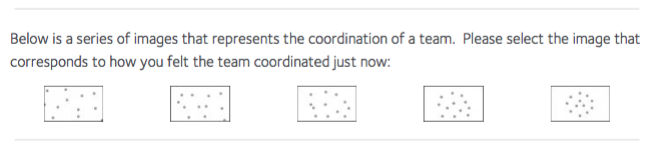
\includegraphics[width = \linewidth]{images/teamClickPictorial.png}
  %    \caption{Click Pictorial Scale}
  %    \label{fig:clickPictorial}
  %  \end{figure}


\myparagraph{Social Bonding\label{app8:bondingPre}}

  \begin{description}
    \item [Emotional Support] ``How emotionally supportive does the team feel?''
    \item [Shared Goal] ``How strong is the feeling that everyone is working towards a shared goal?''
    \item [Group Identification Verbal] A six-item scale designed to measure an individual's personal identification with the stereotypical features of the in-group  \citep{Mael1992}.  All 6 items were measured using a 5-point Likert scale.
          \begin{enumerate}
            \item When someone critises my team, it feels like a personal insult
            \item I am very interested in what others think about my team
            \item When I talk about my team, I usually say ``we'' rather than ``they''
            \item This team's successes are my successes
            \item When someone praises my team, it feels like a personal compliment
            \item If a story in the media criticises my team, I would feel embarrassed
          \end{enumerate}

  \item [Identity Fusion Verbal] A seven-item scale designed to measure an individual's ``feeling of oneness with the group'' \citep{Swann2009}.  Identity Fusion is differentiated from Group Identification in its ability to account for an individual's felt, emotional and personal agentic associations with being a member of the target in-group \citep{Swann2012a}.  All 7 items were measured using a 5-point Likert scale.
    \begin{enumerate}
      \item I am one with my team
      \item I feel immersed in my team
      \item I have a deep emotional bond with my team
      \item My team is me
      \item I’ll do for my team more than any of the other team members would do
      \item I am strong because of my team
      \item I make my team strong
    \end{enumerate}
  \item [Identity Fusion Pictorial] A visual scale designed to measure Identity Fusion to the target in-group \citep{Swann2009}. The pictorial scale depicts two circles, one smaller circle to denote the individual, and one larger circle to denote the group, progressively moving closer to each other such that the most ``fused'' option depicts the smaller circle encased by the larger circle. The scale offers a total of five options to chose from, see Figure ~\ref{fig:fusionPictorialGroup}.  A total of three pictorial scales were included, each with different target in-groups: team, family, and country (China).
  \item [Fusion Pictorial Rank] Athletes were asked to rank their fusion to team, family, and country \citep{Whitehouse2014}.  ``Thinking about these relationships [to team, family, and country] please rank them below in order of which you feel most connected to. 1 for most connected, 3 for least connected.''
  \end{description}


\myparagraph{Subjective and Objective measures of technical competence\label{app8:technicalCompetence}}
Athletes were asked about their individual technical competence: ``Rate your individual ability in rugby,'' relative to:
\begin{enumerate}
  \item Other teammates currently in your team
  \item Other current professional Chinese rugby players
  \item Professional rugby players form other countries
\end{enumerate}
Items were measured with a zero-centred 100 point scale, -50 - ``Extremely weak'', 0 - ``Average'', 50 - ``Extremely strong'').

 %Athletes were also asked about perceived competence of their team relative to other Chinese provincial teams: ``Rate your team's overall ability, relative to other teams in China'' (100 point scale, -50 - ``Extremely weak'', 0 - ``Average'', 50 - ``Extremely strong'').

 %In addition, athletes were asked if their perception of recent performance influences their 1) mood and 2) confidence regarding future performance (All these items were measured with a zero-centred 100 point scale, -50 - ``Extremely weak'', 0 - ``Average'', 50 - ``Extremely strong'').

Athletes were asked to report rugby-related attributes that would provide a more objective indicator of technical competence. These measures included: 1) rugby training age (number of years of experience training for rugby, to the nearest number of years), 2) the number of years spent training with the provincial teams (to the nearest year), 3) whether the athlete is a usual member of the provincial program's starting team or the reserves.


\myparagraph{Ten Item Personality Index\label{app8:TIPI}}
Athletes were asked to indicate on a 7-point Likert scale the extent to which they agreed with 10 pairs of adjectives as appropriate descriptions of their personality. For example: ``I see myself as: dependable, self-disciplined'' (Response: 1 - ``Disagree strongly'', 2 - ``Disagree moderately'',  3 - ``Disagree a little'', 4 - ``Neither agree nor disagree'', 5 - ``Agree a little'', 6 - ``Agree moderately'', 7 - ``Agree strongly''). In the TIPI, two survey items corresponded to each of the big-five personality types, as follows:

\begin{description}
\item [Extraversion:] 1. Extraverted, enthusiastic; 6. Reserved, quiet (Reversed scale)
\item [Agreeableness:] 2. Critical, quarrelsome (Reversed); 7. Sympathetic, warm
\item [Conscientiousness:] 3. Dependable, self-disciplined; 8. Disorganised, careless (Reversed)
\item [Emotional Stability:] 4. Anxious, easily upset (Reversed); 9. Calm, emotionally stable.
\item [Openness to Experiences:] 5. Open to new experiences, complex; 10.Conventional, uncreative (Reversed)
\end{description}


\myparagraph{Injury Status \label{app8:injuryStatus}}
Athletes responded to a question item asking about their injury status: ``Currently, are you physically able participate in a game?'' (100-point scale (0 = ``Unable to play'', 100 = ``Completely fit to play'').

\myparagraph{Team Discipline\label{app8:teamDisciplinePre}}
Athletes were asked about their feelings regarding their team's commitment to aspects of team discipline over the past month (punctuality to training and team meetings, observing bed times and curfews, attendance at meals, general team conduct) (100 point scale for each item, 0 - ``Extremely poor'', 100 - ``Extremely strong'')).


\myparagraph{Identification Variables\label{app8:IDVariables}}
In addition to the items mentioned in the main text, Athletes also reported their date of birth, team affiliation, usual playing position (forward or back), contract and athlete status.






\subsubsection{Mid-Tournament Survey Items\label{app8:surveyMid}}

\myparagraph{Performance\label{app8:performMid}}
\begin{description}
\item [Individual Performance Expectations]``Overall, how do you feel about your individual performance in this game?''
\item [Team Performance Expectations] ``Overall, how do you feel about your team's performance in this game?''
\end{description}
Both items used a zero-centred continuous scale, -50 = ``much worse than expected'', 0 =  ``As expected'', 50 =  ``much better than expected''.

\myparagraph{Arousal, Exertion, and Fatigue\label{app8:exertionMid}}
Following each mid-Tournament survey and in the post-Tournament survey, Athletes were asked to report on various components of physical and mental fatigue, exertion, and injury. Athletes were asked about their mood (``How are you feeling now after the tournament?'') and responded by choosing a point on a 10-point scale between three pairs of emotions (``Not aroused / highly aroused'',  ``Depressed/Relaxed'' and  ``Nervous/Excited'').  Athletes were also asked about feelings of fatigue ``How fatigued do you feel as a result of the game/tournament?'', perceived physical exertion (Borg RPE scale, \citep{Borg1990} and perceived mental exertion using two 15-point scales \citep[see][ ]{Noakes2012a}.  Athletes were also asked to indicate their injury status on a 100-point scale (0 = ``Unable to play'', 100 = ``Completely fit to play'').




\subsubsection{Post-Tournament Survey Items\label{app8:surveyPost}}
The post-Tournament survey repeated the mid-Tournament items, asking:
\begin{description}
\item [Individual Performance Expectations] ``Overall, how do you feel about your individual performance during the tournament?''
\item [Team Performance Expectations]``Overall, how do you feel about your team's performance during the tournament?''
\end{description}

\subsubsection{Objective Performance Measures\label{app8:objectivePerformance}}

\begin{description}
\item [Final Rank:] A rank was given to each team based on performance in their respective competition (men's and women's). These rank scores were then reversed for the purposes of statistical analysis (1st place in men's Tournament (8 teams) = 8, 2nd place = 7, and so on)
\item [Total Wins - Losses:] A team's total number of losses was subtracted from its total number of wins.  Thus, more successful teams overall had a higher score.
\item [Total Minutes:] Total number of minutes played throughout the Tournament by each individual athlete
\item [Total Points:] Total number of points scored throughout the Tournament by each individual athlete
\item [Starting Team Average] An average measure indicating likelihood of an athlete being selected in the starting team. Each Athlete was awarded 1 point for each game he or she started in the starting team; reserve squad athletes were awarded zero for each game. Each athlete's total was divided by the total number of games that they participated in during the Tournament, including games in which they didn't take the field, to produce an average score for the Tournament.
\end{description}







\section{Data Analysis\label{app8:dataAnalysis}}




\subsection{Data reduction\label{app8:dataReduction}}


\subsection{Exploratory Factor Analysis\label{app8:EFA}}
EFA is one of various available data reduction techniques, and is distinct from its main alternative, Principal Components Analysis (PCA), in that it is capable of modelling the latent dimensions of a collection of variables. PCA is concerned only with establishing which components exist within the existing data and how a particular variable might contribute that component. To do this, PCA makes the assumption that all variance in a subset of variables is common variance, and therefore communality between all variables is equal to 1. From this assumption, the original data can be transposed into a linear model without the need for a communality-dependent estimated coefficient for each variable \citep{Widaman2007}. EFA examines all the pairwise relationships between individual variables and seeks to extract latent factors from the measured variables.  Squared Multiple Correlations (which are essentially multiple regressions in which each variable is predicted by all others) were used to calculate the common variance (communality) between each variable in an analysis (the communality value is much like an R-squared value from a multiple regression).
The square root of the communality score for each variable is then used as a coefficient that conditions the relationship between each variable and the underlying dimensions (factors) identifiable in the data. Also known as ``factor loadings,'' these coefficients become the parameters of linear model capable of estimating factor scores for each individual observation, which can be utilised in subsequent statistical analysis in place of single variable observations.

A final step in the EFA procedure is the process of ``rotation'', which is an optimisation technique designed to encourage each variable to load on as few factors as possible \citep{Rummel1988}. Rotation refers to a geometric conception of factor analysis, in which individual variables can be plotted in n-dimensional space according to their relationship to each dimension (factor). By rotating the axes of these dimensions, the distance of a given variable to that dimension can be reduced, which results in an increase in factor loading on one factor and (ideally) a decrease in factor loading on another uncorrelated variable. Orthogonal (or perpendicular) rotation of axes refers to axes, say X and Y, maintaining a 90-degree perpendicularity and rotating clockwise or anticlockwise, depending on the location of the variable clusters.
Orthogonal rotation thus enables optimisation of loadings for clusters of variables that are distant from each other in n-dimensional space. If correlation exists between clusters of variables, however, rotating axes obliquely (inwards towards each other) provides a more effective way of reducing the distance between clusters of variables and the latent dimensions that account for such clustering \citep{Osborne2015}. See Figure ~\ref{fig:orthogonalOblique} for a graphical  illustration of the difference between orthogonal and oblique rotation. Given that most variables of interest in the present study were correlated to some degree, I opted for an oblique rotation method \citep{Field2012}. EFAs were conducted using the factanal() function in the Stats package (Version 3.3.0) in R, using the ``promax'' (oblique) rotation method \citep{Gorsuch1983}. Factor scores were calculated as standardised z-scores: zero-centred, with a standard deviation of 1.

\begin{figure}[htbp]
  \begin{center}
    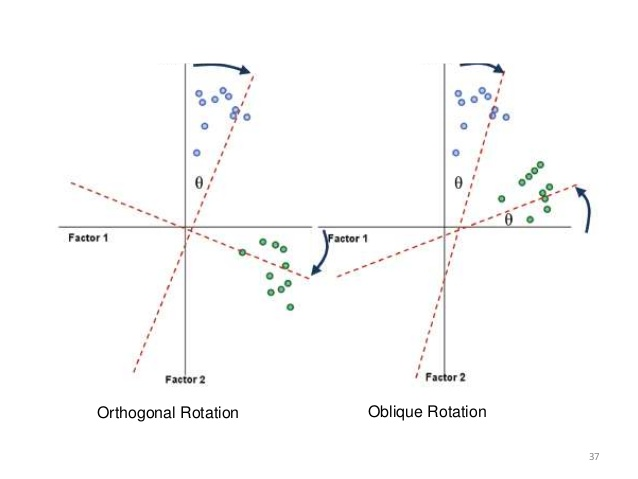
\includegraphics[width= \linewidth, scale = .5]{images/orthogonalObliqueRotationExample.jpg}
    \caption{Orthogonal and oblique rotation methods}
    \label{fig:orthogonalOblique}
  \end{center}
\end{figure}


\subsubsection{Sampling adequacy measures: KMO and Bartlett's Test for Sphericity \label{app8:samplingAdequacy}}

The KMO index provides a proportion measure of common variance to partial correlations among examined variables.  If the KMO index is high ($\approx$ 1), the EFA can act efficiently; if KMO is low ($\approx$ 0), the proposed EFA is not suitable for analysis.

Bartlett’s test of sphericity is used to test the null hypothesis that the correlation matrix is an identity matrix (i.e., a square matrix in which all the elements of the principal diagonal are equal to 1, and all other elements are 0s).

\subsubsection{Reliability measures: Cronbach's alpha and Guttman's lambda3\label{app8:reliabilityMeasures}}

Cronbach's $\alpha$ is a function of the number of items in a test, the average covariance between item-pairs, and the variance of the total score \citep{Tabachnick2007}



\subsection{Model Selection\label{app8:modelSelection}}
Due to the dependencies in the data and missingness throughout, both traditional ANCOVA (analysis of co-variance) models linear mixed-effects regression models (LMER) are capable of incorporating both fixed and random effects into analysis of variance, however ANCOVA designs only allow the intercept (and not the regression slope) to vary according to level-2 variance, whereas LMER can model the variability of both intercept and slope across different groups of the predictor variable \citep{Field2012}. In addition, the ability of LMERs to deal with unbalanced designs (due to missing values) meant that a LMER was the most suitable modelling strategy for the present study.

\subsubsection{Judging robustness: normality of residuals\label{app8:normality}}
Non-normally distributed residuals are problematic as they may influence the model's ability to generate accurate parameter estimates . Two data manipulation techniques were considered in order to normalise residuals and therefore preserve the estimates of the model: 1) exclusion of outliers \citep[according to Tukey's method; observations above and below 1.5x the Inter Quartile Range (IQR); see][]{Tukey1977}) and 2) transformation of the outcome variable.  Transformation of the outcome variables was the preferred method over outlier exclusion, due to the cost involved in removing observations that may be of potential theoretical relevance to the scientific investigation \citep{Rousseeuw2011}.

\subsubsection{Intra-class correlation\label{app8:ICC}}
To assess the need for a statistical model capable of accounting for correlation of residuals, dependency in the data a was quantified using a ratio measure comparing within- and between-group variance, known as the intra-class correlation (ICC). Clustering in the data according to team or sex (the separate men's and women's Tournament) was considered.

For team-level variance, a one-way random effects model was used, in which average within-team variance (Mean Square Within) of the response variable was divided by the average total variance of the response (Mean Square Total) \citep{Field2005a}.  Each athlete was member of one of 15 teams, which were considered to be sampled from a larger pool of potential teams, hence treated as random effects. The ICC was then interpreted as the percentage of total variance accounted for by group-level variables \citep{Wolak2012}.
To statistically account for the unbalanced design of the data, an adjusted sample-size coefficient (k) was calculated using an equation provided by \citep{Lessells1987}.  While there is no firm agreement on what is deemed meaningful within-group variance, an ICC ratio of $>.10-1.00$ with confidence intervals that do not include zero was considered an indication of non-random correlation of group-level residuals \citep{Bailey2011}. As Table ~\ref{tab:ICCsummaryTeam} and ~\ref{tab:ICCsummarySex} indicate, small to moderate team-level intra-class correlation of responses exist for factors of Objective Competence, Team Performance Components, Individual Performance Success, and Team Click.  ICCs for Social Bonding and Fatigue meanwhile were relatively low (all $r's <.1$). Sex-level ICCs were all relatively low, suggesting that sex-level variation could be ignored in subsequent inferential analyses.\\


% Table created by stargazer v.5.2 by Marek Hlavac, Harvard University. E-mail: hlavac at fas.harvard.edu
% Date and time: Sun, Jun 25, 2017 - 21:23:24
\begin{table}[!htbp] \centering 
  \caption{Intra-Class Correlations for post-Tournament Factors according to team} 
  \label{tab:ICCsummaryTeam} 
\small 
\begin{tabular}{@{\extracolsep{5pt}} cccccc} 
\\[-1.8ex]\hline 
\hline \\[-1.8ex] 
 & variable & ICC.team & LowerCI.team & UpperCI.team & k.adjusted.team \\ 
\hline \\[-1.8ex] 
1 & subjectiveCompetence & $0.011$ & $$-$0.057$ & $0.185$ & $8.476$ \\ 
2 & objectiveCompetence & $0.356$ & $0.175$ & $0.625$ & $8.476$ \\ 
3 & jointActionSuccess & $0.374$ & $0.190$ & $0.634$ & $7.768$ \\ 
4 & indPerformanceSuccess & $0.223$ & $0.074$ & $0.484$ & $7.768$ \\ 
5 & teamClick & $0.299$ & $0.130$ & $0.564$ & $7.768$ \\ 
6 & socialBonding & $0.098$ & $$-$0.010$ & $0.324$ & $7.768$ \\ 
7 & fatigue & $0.056$ & $$-$0.036$ & $0.261$ & $7.768$ \\ 
\hline \\[-1.8ex] 
\end{tabular} 
\end{table} 


% Table created by stargazer v.5.2 by Marek Hlavac, Harvard University. E-mail: hlavac at fas.harvard.edu
% Date and time: Sun, Jun 25, 2017 - 21:23:23
\begin{table}[!htbp] \centering 
  \caption{Intra-Class Correlations for post-Tournament Factors according to sex} 
  \label{tab:ICCsummarySex} 
\small 
\begin{tabular}{@{\extracolsep{5pt}} cccccc} 
\\[-1.8ex]\hline 
\hline \\[-1.8ex] 
 & variable & ICC.sex & LowerCI.sex & UpperCI.sex & k.adjusted.sex \\ 
\hline \\[-1.8ex] 
1 & subjectiveCompetence & $0.039$ & $$-$0.006$ & $0.983$ & $58.933$ \\ 
2 & objectiveCompetence & $0.092$ & $0.006$ & $0.992$ & $58.933$ \\ 
3 & jointActionSuccess & $$-$0.017$ & $$-$0.017$ & $0.014$ & $58.390$ \\ 
4 & indPerformanceSuccess & $0.108$ & $0.009$ & $0.993$ & $58.390$ \\ 
5 & teamClick & $$-$0.010$ & $$-$0.016$ & $0.881$ & $58.390$ \\ 
6 & socialBonding & $0.079$ & $0.003$ & $0.991$ & $58.390$ \\ 
7 & fatigue & $0.023$ & $$-$0.009$ & $0.976$ & $58.390$ \\ 
\hline \\[-1.8ex] 
\end{tabular} 
\end{table} 



\subsubsection{Mediation Analysis\label{app8:mediationAnalysis}}
A formal mediation analysis can be used to test the prediction that the relationship between perceptions of joint-action success and social bonding is mediated by feelings of team click, by analysing if and how an intervening variable is causally significant to the relationship between a predictor and an outcome variable. A variable is a mediator if it carries the influence of the predictor variable to an outcome variable, if it serves to explain (either partially or fully) the variance in the outcome variable attributable to the predictor. In the case of this analysis, do perceptions of joint-action success have an indirect effect on feelings of social bonding that is transmitted through feelings associated with team click?

\begin{figure}[htbp]
  \begin{center}
    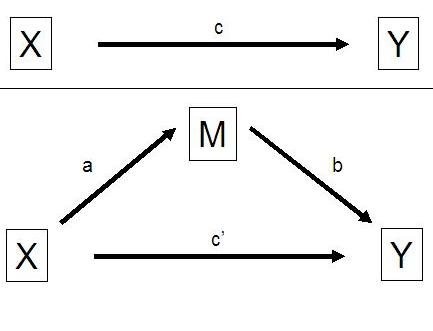
\includegraphics[scale = .5]{images/mediation_image.jpg}
    \caption{Mediation Analysis: direct and indirect effects}
    \label{fig:mediationAnalysis}
  \end{center}
\end{figure}

Mediation analysis works by testing the extent to which the variance in the outcome attributable to a predictor variable (the direct effect, or path ``c'': $Y_i \sim d_Y + cX_i + e_i$) can be explained \textit{indirectly} by the variance of two other relationships: that of the predictor variable and a third mediator (X $\rightarrow$ M, or path ``a'')  and M and the outcome variable (path ``b''), controlling for the direct relationship between X and Y (path ``'c'') (see Figure ~\ref{fig:mediationAnalysis}). The mediation model can thus be denoted by two equations:

\begin{equation}
  M_i \sim d_M + aX_i + e_Mi
\end{equation}

\begin{equation}
  Y_i \sim d_Y + bM_i + c'X_i +  + e_{Yi}
\end{equation}
\bigskip

When combined, these two equations enable the calculation of the ``indirect effect'' of the predictor on the outcome, by controlling for the relationship between the mediator's effect on the outcome variable as a function of its relationship to the predictor variable.  While the direct effect measures the extent to which the dependent variable changes when the independent variable increases by one unit and the mediator variable remains unaltered, the indirect effect measures the extent to which the dependent variable changes when the independent variable is held fixed and the mediator variable changes by the amount it would have changed had the independent variable increased by one unit \citep{Bauer2006}.

The multilevel structure of the data in this study, i.e. the clustering of residuals according to team affiliation, violates the independence assumption of mediation analysis. As such, traditional multiple linear regression and path analysis will produce biased tests of the effects in the mediation model \citep{Raudenbush2002}.
%(Hox, 2002; Kreft & de Leeuw, 1998; Raudenbush & Bryk, 2002).
A multilevel mediation analysis must therefore additionally take into account variance attributable to the random effects of the model (team, in this case), and in so doing capture heterogeneity of variance in the indirect effect due to the level 2 variable \citep{Tofighi2014}.  To do this, each coefficient in the model must be random (denoted by subscript ``j''), so that the value of the coefficient varies across Level 2 units (team): \\

\begin{equation}
  M_{ij} \sim d_{Mj} + a_jX_{ij} + e_{Mij}
\end{equation}

\begin{equation}
  Y_{ij} \sim d_{Yj} + b_jM_{ij} + 'c_jX_{ij} +  + e_{Yij}
\end{equation}
\bigskip

Linear mixed effects regression models are fitted according to these equations, and estimates of mediation effects can be computed from these model parameters.  Subsequent mediation analyses were conducted using the ``mediation'' function of the Causal Mediation Analysis Package (version 4.4.5) in R.









\section{Results\label{app8:results}}



\subsection{Descriptive Statistics}

\subsubsection{Pre-Tournament Data Descriptives \label{app8:descriptivesPre}}

\begin{table}[htpb]\caption{Summary Statistics: post-Tournament Technical Competence (objective and subjective)}
\begin{center}
\begin{small} 
\begin{tabular}
{l
r
r
r
r
r
r
r
}

\multicolumn{
7
}{l}{

}
\cr 
 \hline 
Variable  &  
n  & 
mean  & 
sd  & 
min  & 
max  & 
skew  & 
krtss \cr 

 \hline 

Years In Team   &  120  &   3.17  &   2.12  &    0  &   7  &   0.29  &  -1.25 \cr 

Training Age   &  120  &   4.40  &   2.35  &    0  &  13  &   0.47  &   0.66 \cr 

Starting Team Average   &  172  &   0.61  &   0.36  &    0  &   1  &  -0.43  &  -1.32 \cr 

Age   &  121  &  21.67  &   3.26  &   16  &  32  &   0.52  &  -0.27 \cr 

Ability Teammates   &  120  &  19.45  &  20.14  &  -40  &  50  &  -0.31  &  -0.56 \cr 

Ability Chinese Pros   &  120  &  15.78  &  19.59  &  -35  &  50  &  -0.18  &  -0.65 \cr 

Ability International   &  120  &  18.46  &  26.19  &  -44  &  50  &  -0.48  &  -0.77 \cr 

Team Ability China   &  120  &  22.48  &  22.90  &  -40  &  50  &  -0.64  &  -0.58 \cr 

 \hline 
\end{tabular}
\end{small}
\end{center}
\label{tab:1competenceDescriptives}
\end{table} 




Table ~\ref{tab:1competenceDescriptives} displays the variables relevant to an Athlete's technical competence.  These variables were collected in the pre-Tournament survey, and as such the number of observations per variable is generally 120, except for ``Starting Team Average,'' which was generated from the objective performance data provided by CRFA following the Tournament.  The average number of years in the team was over three years, and the average training age for Athletes was 4.4 years.  In terms of subjective confidence, means for each variable were well above the mid-point of the scale, suggesting that Athletes were on average quite positive about their own ability compared to other athletes (their teammates, other Chinese professionals, International professionals).

%\subsubsection{Mid-Tournament Data}



\subsubsection{Post-Tournament Data}

%
% Table created by stargazer v.5.2 by Marek Hlavac, Harvard University. E-mail: hlavac at fas.harvard.edu
% Date and time: Mon, Jun 26, 2017 - 09:48:21
\begin{table}[!htbp] \centering 
  \caption{Overall Tournament Performance Summary Statistics} 
  \label{tab:performanceOverallSummary} 
\scriptsize 
\begin{tabular}{@{\extracolsep{5pt}} ccccccccc} 
\\[-1.8ex]\hline 
\hline \\[-1.8ex] 
time & teamPerf & tP.sd & indPerf & iP.sd & teamPerfExp & tPE.sd & indPerfExp & iP.sd.1 \\ 
\hline \\[-1.8ex] 
pre-Tournament & $71.11$ & $21.87$ & $68.92$ & $21.32$ & $$ & $$ & $$ & $$ \\ 
day1 & $$ & $$ & $$ & $$ & $54.43$ & $30.63$ & $39.43$ & $27.25$ \\ 
day2 & $$ & $$ & $$ & $$ & $53.19$ & $32.98$ & $40.92$ & $27.93$ \\ 
post-Tournament & $$ & $$ & $$ & $$ & $64.36$ & $23.61$ & $56.36$ & $23.47$ \\ 
\hline \\[-1.8ex] 
\end{tabular} 
\end{table} 

%
% Table created by stargazer v.5.2 by Marek Hlavac, Harvard University. E-mail: hlavac at fas.harvard.edu
% Date and time: Mon, Jun 26, 2017 - 09:21:29
\begin{table}[!htbp] \centering 
  \caption{Team Click Overall Tournament Summary Statistics} 
  \label{tab:clickOverallSummary} 
\scriptsize 
\begin{tabular}{@{\extracolsep{5pt}} ccccccc} 
\\[-1.8ex]\hline 
\hline \\[-1.8ex] 
time & unspUnd & uU.sd & genAt & gA.sd & clickPic & cP.sd \\ 
\hline \\[-1.8ex] 
pre-Tournament & $71.58$ & $20.77$ & $75.51$ & $23.27$ & $3.87$ & $1.24$ \\ 
day1 & $55.92$ & $26.88$ & $65.74$ & $31.95$ & $3.46$ & $1.49$ \\ 
day2 & $55.30$ & $29.43$ & $64.32$ & $33.39$ & $3.33$ & $1.70$ \\ 
post-Tournament & $72.72$ & $19.95$ & $78.45$ & $21.34$ & $3.93$ & $1.04$ \\ 
\hline \\[-1.8ex] 
\end{tabular} 
\end{table} 

%
% Table created by stargazer v.5.2 by Marek Hlavac, Harvard University. E-mail: hlavac at fas.harvard.edu
% Date and time: Mon, Jun 26, 2017 - 09:22:14
\begin{table}[!htbp] \centering 
  \caption{Social Bonding Overall Tournament Summary Statistics} 
  \label{tab:bondingOverallSummary} 
\scriptsize 
\begin{tabular}{@{\extracolsep{5pt}} ccccccc} 
\\[-1.8ex]\hline 
\hline \\[-1.8ex] 
time & emoSup & eS.sd & sharedGoal & sG.sd & fusionPic & fP.sd \\ 
\hline \\[-1.8ex] 
pre-Tournament & $70.12$ & $26.21$ & $77.66$ & $24.28$ & $4.26$ & $1.25$ \\ 
day1 & $67.29$ & $30.56$ & $76.34$ & $30.50$ & $4.06$ & $1.47$ \\ 
day2 & $67.53$ & $32.55$ & $71.42$ & $35.47$ & $3.85$ & $1.69$ \\ 
post-Tournament & $79.67$ & $18.84$ & $86$ & $15.56$ & $4.33$ & $1.19$ \\ 
\hline \\[-1.8ex] 
\end{tabular} 
\end{table} 

%
% Table created by stargazer v.5.2 by Marek Hlavac, Harvard University. E-mail: hlavac at fas.harvard.edu
% Date and time: Mon, Jun 26, 2017 - 09:23:43
\begin{table}[!htbp] \centering 
  \caption{Fatigue Overall Tournament Summary Statistics} 
  \label{tab:fatigueOverallSummary} 
\scriptsize 
\begin{tabular}{@{\extracolsep{5pt}} ccccccccc} 
\\[-1.8ex]\hline 
\hline \\[-1.8ex] 
time & fat & f.sd & prpe & p.sd & mental & m.sd & inj.mu & inj.sd \\ 
\hline \\[-1.8ex] 
pre-Tournament & $$ & $$ & $$ & $$ & $$ & $$ & $18.73$ & $23.36$ \\ 
day1 & $50.14$ & $28.80$ & $12.45$ & $4.52$ & $4.09$ & $2.83$ & $29.91$ & $33.15$ \\ 
day2 & $53.65$ & $31.03$ & $12.60$ & $5.53$ & $4.13$ & $3.17$ & $37.14$ & $37.66$ \\ 
post-Tournament & $69.27$ & $21.24$ & $14.97$ & $2.66$ & $6.08$ & $2.47$ & $23.86$ & $26.91$ \\ 
\hline \\[-1.8ex] 
\end{tabular} 
\end{table} 



%\begin{table}[htpb]\caption{Summary Statistics: post-Tournament Performance (individual and team)}
\begin{center}
\begin{small} 
\begin{tabular}
{l
r
r
r
r
r
r
r
}

\multicolumn{
7
}{l}{

}
\cr 
 \hline 
Variable  &  
{n} & 
{mean} & 
{sd} & 
{min} & 
{max} & 
{skew} & 
{krtss}\cr 

 \hline 

indPerformance7   &  118  &  56.36  &  23.47  &  0  &  100  &  -0.35  &  -0.08 \cr 

passingTech7   &  118  &  58.41  &  24.25  &  0  &  100  &  -0.79  &   0.05 \cr 

supportAttack7   &  118  &  62.62  &  22.70  &  0  &  100  &  -0.98  &   0.64 \cr 

indDefense7   &  118  &  57.64  &  23.57  &  0  &  100  &  -0.55  &  -0.11 \cr 

effectContact7   &  118  &  62.15  &  24.81  &  0  &  100  &  -0.97  &   0.40 \cr 

decisionAttack7   &  118  &  61.22  &  21.43  &  0  &  100  &  -0.72  &   0.37 \cr 

teamPerformance7   &  118  &  64.36  &  23.61  &  0  &  100  &  -0.52  &  -0.30 \cr 

teamDefense7   &  118  &  62.42  &  22.50  &  0  &  100  &  -0.52  &  -0.52 \cr 

teamAttack7   &  118  &  65.33  &  20.26  &  0  &  100  &  -0.53  &  -0.23 \cr 

teamSupportPlay7   &  118  &  65.75  &  19.72  &  0  &  100  &  -0.76  &   0.57 \cr 

teamCommunication7   &  118  &  65.25  &  21.26  &  0  &  100  &  -0.65  &   0.27 \cr 

 \hline 
\end{tabular}
\end{small}
\end{center}
\label{tab:2performancePostDescriptives}
\end{table} 



%\begin{table}[htpb]\caption{Summary Statistics: post-Tournament Team Click}
\begin{center}
\begin{small} 
\begin{tabular}
{l
r
r
r
r
r
r
r
}

\multicolumn{
7
}{l}{

}
\cr 
 \hline 
Variable  &  
{n} & 
{mean} & 
{sd} & 
{min} & 
{max} & 
{skew} & 
{krtss}\cr 

 \hline 

unspokenUnderstanding7   &  118  &  72.72  &  19.95  &  0  &  100  &  -1.38  &  2.13 \cr 

generalAtmosphere7   &  118  &  78.45  &  21.34  &  0  &  100  &  -1.51  &  2.82 \cr 

clickPictorial7   &  118  &   3.93  &   1.04  &  1  &    5  &  -0.78  &  0.00 \cr 

reliabilityOfOthers7   &  118  &  68.00  &  23.09  &  0  &  100  &  -1.33  &  1.75 \cr 

reliabilityForOthers7   &  118  &  63.45  &  25.80  &  0  &  100  &  -1.06  &  0.51 \cr 

abilityExtended7   &  118  &  72.25  &  19.27  &  0  &  100  &  -1.13  &  2.03 \cr 

 \hline 
\end{tabular}
\end{small}
\end{center}
\label{tab:3clickPostDescriptives}
\end{table} 



%\begin{table}[htpb]\caption{Summary Statistics: post-Tournament Social Bonding}
\begin{center}
\begin{small} 
\begin{tabular}
{l
r
r
r
r
r
r
r
}

\multicolumn{
7
}{l}{

}
\cr 
 \hline 
Variable  &  
{n} & 
{mean} & 
{sd} & 
{min} & 
{max} & 
{skew} & 
{krtss}\cr 

 \hline 

emotionalSupport7   &  118  &  79.67  &  18.84  &   0.00  &  100  &  -1.74  &  4.37 \cr 

sharedGoal7   &  118  &  86.00  &  15.56  &  29.00  &  100  &  -1.38  &  2.24 \cr 

groupId7   &  118  &   4.29  &   0.67  &   1.50  &    5  &  -1.18  &  1.66 \cr 

fusionVerbal7   &  118  &   4.00  &   0.71  &   1.43  &    5  &  -0.86  &  0.99 \cr 

fusionPictorialTeam7   &  118  &   4.33  &   1.19  &   0.00  &    5  &  -2.45  &  6.07 \cr 

fusionPictorialFamily7   &  118  &   4.51  &   0.96  &   0.00  &    5  &  -2.30  &  5.62 \cr 

fusionPictorialCountry7   &  118  &   4.03  &   1.39  &   0.00  &    5  &  -1.59  &  1.84 \cr 

 \hline 
\end{tabular}
\end{small}
\end{center}
\label{tab:4bondingPostDescriptives}
\end{table} 




%\begin{table}[htpb]\caption{Summary Statistics: post-Tournament measures of fatigue}
\begin{center}
\begin{small} 
\begin{tabular}
{l
r
r
r
r
r
r
r
}

\multicolumn{
7
}{l}{

}
\cr 
 \hline 
Variable  &  
n  & 
mean  & 
sd  & 
min  & 
max  & 
skew  & 
krtss \cr 

 \hline 

Fatigue   &  118  &  69.27  &  21.24  &   0  &  100  &  -1.13  &  1.40 \cr 

RPE(physical)   &  118  &  14.97  &   2.66  &   6  &   20  &  -0.80  &  0.49 \cr 

RPE(mental)   &  118  &   6.08  &   2.47  &  -4  &   10  &  -1.13  &  1.82 \cr 

injuryRev7   &  118  &  23.86  &  26.91  &   0  &  100  &   1.19  &  0.60 \cr 

 \hline 
\end{tabular}
\end{small}
\end{center}
\label{tab:5fatiguePostDescriptives}
\end{table} 






\begin{table}[htpb]\caption{Summary Statistics: Objective Tournament Performance}
\begin{center}
\begin{small} 
\begin{tabular}
{l
r
r
r
r
r
r
r
}

\multicolumn{
7
}{l}{

}
\cr 
 \hline 
Variable  &  
n  & 
mean  & 
sd  & 
min  & 
max  & 
skew  & 
krtss \cr 

 \hline 

Final Rank   &  174  &   4.83  &   2.15  &   1  &   8  &  -0.09  &  -1.17 \cr 

Wins - Losses   &  172  &   0.32  &   2.94  &  -6  &   6  &  -0.17  &  -0.25 \cr 

Total Ind Points   &  172  &   8.45  &  11.41  &   0  &  69  &   2.34  &   7.23 \cr 

Total Ind Minutes   &  172  &  44.01  &  20.65  &   1  &  81  &  -0.38  &  -0.89 \cr 

Starting Team Avg   &  172  &   0.61  &   0.36  &   0  &   1  &  -0.43  &  -1.32 \cr 

 \hline 
\end{tabular}
\end{small}
\end{center}
\label{tab:6objectiveTournamentDescriptives}
\end{table} 




Table ~\ref{tab:2performancePostDescriptives} shows that the central tendency for individual and team performance measures was well above the mid-point of the scale, with team performance items slightly higher that individual performance items.  This negatively skewed central tendency in survey responses was more pronounced for variables relating to team click (as Table ~\ref{tab:3clickPostDescriptives} indicates), with the central tendency for each variable ranging between 65 and 78 (100-point scale, SD range = 19-27). The exception to this was the 5-point Team Click Pictorial Scale, the average for which was 3.93 (out of 5, SD = 1.04).  All six items relating to team click had a pronounced negative skew.  As Table ~\ref{tab:4bondingPostDescriptives} demonstrates, the trend for bonding was even higher; central tendencies for Emotional Support and Shared Goal were 79.67 (SD = 18.84) and 86 (SD = 15.56) respectively.  Group Identification Verbal Scale, and Identity Fusion Verbal and Pictorial Scales (5-point Likert) also had a high negatively skewed distribution, with central tendencies between 4 (Identity Fusion Verbal, SD = .71) and 4.51 (Identity Fusion Family, SD = 0.96).
In addition to these main variables of interest, the central tendency of distributions of responses related to arousal, exertion, and fatigue were also well above the mid-point of their respective scales (see Table ~\ref{tab:5fatiguePostDescriptives}).  Table ~\ref{tab:6objectiveTournamentDescriptives} displays athlete objective performance in the Tournament. Athletes played an average of 44 minutes of rugby during the Tournament (just under four full games each), and each Athlete scored an average of 8.45 points, which amounts to between one and two tries each, or a number of try drop-kick conversions (worth two points each).








\subsection{Data Reduction}


%\subsubsection{Performance: team and individual\label{app8:performanceDataReduction}}



%\myparagraph{Pre- to Post-Tournament}

%$\chi^2 (df=2) = 20.27$, $p < .001$,
%$\chi^2 (df=5) = 47.29$, $p < .001$,



%Summary statistics for the factors extracted from the Post-Tournament data, and their correlations can be viewed in Appendix ~\ref{app8:tournamentSurvey} Section
 %~\ref{tab:postTournamentFactorDescriptives} and Table ~\ref{tab:postTournamentFactorCorr} respectively.



%%\newpage
%\newgeometry{margin=0.5cm} % modify this if you need even more space
%\begin{landscape}
    %
% Table created by stargazer v.5.2.2 by Marek Hlavac, Harvard University. E-mail: hlavac at fas.harvard.edu
% Date and time: Mon, Aug 27, 2018 - 18:51:00
\begin{table}[!htbp] \centering 
  \caption{Correlation Matrix: post-Tournament Technical Competence} 
  \label{tab:1competenceCorr} 
\scriptsize 
\begin{tabular}{@{\extracolsep{5pt}} ccccccccc} 
\\[-1.8ex]\hline 
\hline \\[-1.8ex] 
 & Years In Team & Training Age & Starting Team Average & Age & Ability Teammates & Ability Chinese Pros & Ability International & Team Ability China \\ 
\hline \\[-1.8ex] 
Years In Team & $1$ & $0.510$ & $$-$0.044$ & $0.569$ & $0.076$ & $0.102$ & $0.099$ & $0.261$ \\ 
Training Age & $0.510$ & $1$ & $0.0004$ & $0.697$ & $0.095$ & $0.183$ & $0.201$ & $0.190$ \\ 
Starting Team Average & $$-$0.044$ & $0.0004$ & $1$ & $$-$0.040$ & $0.203$ & $0.099$ & $0.044$ & $0.144$ \\ 
Age & $0.569$ & $0.697$ & $$-$0.040$ & $1$ & $0.132$ & $0.089$ & $0.154$ & $0.212$ \\ 
Ability Teammates & $0.076$ & $0.095$ & $0.203$ & $0.132$ & $1$ & $0.428$ & $0.383$ & $0.454$ \\ 
Ability Chinese Pros & $0.102$ & $0.183$ & $0.099$ & $0.089$ & $0.428$ & $1$ & $0.702$ & $0.273$ \\ 
Ability International & $0.099$ & $0.201$ & $0.044$ & $0.154$ & $0.383$ & $0.702$ & $1$ & $0.212$ \\ 
Team Ability China & $0.261$ & $0.190$ & $0.144$ & $0.212$ & $0.454$ & $0.273$ & $0.212$ & $1$ \\ 
\hline \\[-1.8ex] 
\end{tabular} 
\end{table} 

    %
% Table created by stargazer v.5.2 by Marek Hlavac, Harvard University. E-mail: hlavac at fas.harvard.edu
% Date and time: Sun, Jun 25, 2017 - 21:08:16
\begin{table}[!htbp] \centering 
  \caption{Correlation Matrix: post-Tournament Team Performance} 
  \label{tab:22teamPerformancePostCorr} 
\footnotesize 
\begin{tabular}{@{\extracolsep{5pt}} ccccc} 
\\[-1.8ex]\hline 
\hline \\[-1.8ex] 
 & Team Defence & Team Attack & Team Support Play & Team Onfield Communication \\ 
\hline \\[-1.8ex] 
Team Defence & $1$ & $0.834$ & $0.643$ & $0.721$ \\ 
Team Attack & $0.834$ & $1$ & $0.740$ & $0.713$ \\ 
Team Support Play & $0.643$ & $0.740$ & $1$ & $0.715$ \\ 
Team Onfield Communication & $0.721$ & $0.713$ & $0.715$ & $1$ \\ 
\hline \\[-1.8ex] 
\end{tabular} 
\end{table} 

%    
% Table created by stargazer v.5.2 by Marek Hlavac, Harvard University. E-mail: hlavac at fas.harvard.edu
% Date and time: Sun, Jun 25, 2017 - 21:07:58
\begin{table}[!htbp] \centering 
  \caption{Correlation Matrix: Individual Performance} 
  \label{tab:21indPerformancePostCorr} 
\footnotesize 
\begin{tabular}{@{\extracolsep{5pt}} cccccc} 
\\[-1.8ex]\hline 
\hline \\[-1.8ex] 
 & Passing Tech & Support In Attack & Ind Defence & Effectiveness In Contact & Decision Making Attack \\ 
\hline \\[-1.8ex] 
Passing Tech & $1$ & $0.658$ & $0.510$ & $0.508$ & $0.607$ \\ 
Support In Attack & $0.658$ & $1$ & $0.658$ & $0.641$ & $0.734$ \\ 
Ind Defence & $0.510$ & $0.658$ & $1$ & $0.590$ & $0.525$ \\ 
Effectiveness In Contact & $0.508$ & $0.641$ & $0.590$ & $1$ & $0.713$ \\ 
Decision Making Attack & $0.607$ & $0.734$ & $0.525$ & $0.713$ & $1$ \\ 
\hline \\[-1.8ex] 
\end{tabular} 
\end{table} 

%    
% Table created by stargazer v.5.2.2 by Marek Hlavac, Harvard University. E-mail: hlavac at fas.harvard.edu
% Date and time: Mon, Aug 27, 2018 - 18:51:00
\begin{table}[!htbp] \centering 
  \caption{Correlation Matrix: post-Tournament Team Click} 
  \label{} 
\footnotesize 
\begin{tabular}{@{\extracolsep{5pt}} ccccccc} 
\\[-1.8ex]\hline 
\hline \\[-1.8ex] 
 & unspokenUnderstanding7 & generalAtmosphere7 & clickPictorial7 & reliabilityOfOthers7 & reliabilityForOthers7 & abilityExtended7 \\ 
\hline \\[-1.8ex] 
unspokenUnderstanding7 & $1$ & $0.626$ & $0.508$ & $0.275$ & $0.230$ & $0.375$ \\ 
generalAtmosphere7 & $0.626$ & $1$ & $0.385$ & $0.301$ & $0.276$ & $0.265$ \\ 
clickPictorial7 & $0.508$ & $0.385$ & $1$ & $0.282$ & $0.021$ & $0.213$ \\ 
reliabilityOfOthers7 & $0.275$ & $0.301$ & $0.282$ & $1$ & $0.276$ & $0.544$ \\ 
reliabilityForOthers7 & $0.230$ & $0.276$ & $0.021$ & $0.276$ & $1$ & $0.375$ \\ 
abilityExtended7 & $0.375$ & $0.265$ & $0.213$ & $0.544$ & $0.375$ & $1$ \\ 
\hline \\[-1.8ex] 
\end{tabular} 
\end{table} 


%    \clearpage
%    
% Table created by stargazer v.5.2 by Marek Hlavac, Harvard University. E-mail: hlavac at fas.harvard.edu
% Date and time: Tue, May 30, 2017 - 09:19:43
\begin{table}[!htbp] \centering 
  \caption{Correlation Matrix: post-Tournament Social Bonding} 
  \label{} 
\footnotesize 
\begin{tabular}{@{\extracolsep{5pt}} cccccc} 
\\[-1.8ex]\hline 
\hline \\[-1.8ex] 
 & emotionalSupport & sharedGoal & groupIdentification & identityFusionVerbal & identityFusionPictorialTeam \\ 
\hline \\[-1.8ex] 
emotionalSupport & $1$ & $0.619$ & $0.079$ & $0.331$ & $0.349$ \\ 
sharedGoal & $0.619$ & $1$ & $0.061$ & $0.246$ & $0.395$ \\ 
groupIdentification & $0.079$ & $0.061$ & $1$ & $0.358$ & $0.081$ \\ 
identityFusionVerbal & $0.331$ & $0.246$ & $0.358$ & $1$ & $0.220$ \\ 
identityFusionPictorialTeam & $0.349$ & $0.395$ & $0.081$ & $0.220$ & $1$ \\ 
\hline \\[-1.8ex] 
\end{tabular} 
\end{table} 

%    
% Table created by stargazer v.5.2 by Marek Hlavac, Harvard University. E-mail: hlavac at fas.harvard.edu
% Date and time: Sat, Jun 03, 2017 - 22:22:24
\begin{table}[!htbp] \centering 
  \caption{Correlation Matrix: post-Tournament Fatigue} 
  \label{} 
\footnotesize 
\begin{tabular}{@{\extracolsep{5pt}} ccccc} 
\\[-1.8ex]\hline 
\hline \\[-1.8ex] 
 & fatigue & RPE(physical) & RPE(mental) & injuryRev7 \\ 
\hline \\[-1.8ex] 
fatigue & $1$ & $0.665$ & $0.510$ & $0.090$ \\ 
RPE(physical) & $0.665$ & $1$ & $0.523$ & $0.009$ \\ 
RPE(mental) & $0.510$ & $0.523$ & $1$ & $$-$0.040$ \\ 
injuryRev7 & $0.090$ & $0.009$ & $$-$0.040$ & $1$ \\ 
\hline \\[-1.8ex] 
\end{tabular} 
\end{table} 

%    
% Table created by stargazer v.5.2 by Marek Hlavac, Harvard University. E-mail: hlavac at fas.harvard.edu
% Date and time: Tue, May 30, 2017 - 09:19:44
\begin{table}[!htbp] \centering 
  \caption{Tournament Performance Correlation Matrix} 
  \label{} 
\footnotesize 
\begin{tabular}{@{\extracolsep{5pt}} cccccc} 
\\[-1.8ex]\hline 
\hline \\[-1.8ex] 
 & finalRank & totalWins - totalLosses & totalIndPoints & totalMinutesPlayed & startingTeamAvg \\ 
\hline \\[-1.8ex] 
finalRank & $1$ & $0.901$ & $0.381$ & $0.062$ & $0.055$ \\ 
totalWins - totalLosses & $0.901$ & $1$ & $0.428$ & $0.129$ & $0.089$ \\ 
totalIndPoints & $0.381$ & $0.428$ & $1$ & $0.404$ & $0.067$ \\ 
totalMinutesPlayed & $0.062$ & $0.129$ & $0.404$ & $1$ & $$-$0.038$ \\ 
startingTeamAvg & $0.055$ & $0.089$ & $0.067$ & $$-$0.038$ & $1$ \\ 
\hline \\[-1.8ex] 
\end{tabular} 
\end{table} 


%    \clearpage
    %\begin{table}[htpb]\caption{Summary Statistics: post-Tournament Factors}
\begin{center}
\begin{scriptsize} 
\begin{tabular}
{l
r
r
r
r
r
r
r
}

\multicolumn{
7
}{l}{

}
\cr 
 \hline 
Variable  &  
n  & 
mean  & 
sd  & 
min  & 
max  & 
skew  & 
krtss \cr 

 \hline 

objCompetence   &  120  &   0.00  &   0.95  &  -1.99  &    2.91  &   0.45  &  -0.23 \cr 

subjCompetence   &  120  &   0.00  &   0.96  &  -2.58  &    1.79  &  -0.16  &  -0.66 \cr 

indPerformExp   &  118  &  56.36  &  23.47  &   0.00  &  100.00  &  -0.35  &  -0.08 \cr 

indPerformSuccess   &  118  &   0.00  &   0.95  &  -2.96  &    1.70  &  -0.85  &   0.60 \cr 

teamPerformanceExpect   &  118  &  64.36  &  23.61  &   0.00  &  100.00  &  -0.52  &  -0.30 \cr 

jointActionSuccess   &  118  &   0.00  &   0.96  &  -3.28  &    1.79  &  -0.49  &  -0.01 \cr 

teamClick   &  118  &   0.00  &   0.90  &  -3.06  &    1.42  &  -1.01  &   1.03 \cr 

socialBonding   &  118  &   0.00  &   0.89  &  -3.08  &    1.08  &  -1.38  &   2.00 \cr 

fatigue   &  118  &   0.00  &   0.91  &  -3.40  &    1.67  &  -1.03  &   1.56 \cr 

 \hline 
\end{tabular}
\end{scriptsize}
\end{center}
\label{tab:postTournamentFactorDescriptives}
\end{table} 



%\end{landscape}
%\restoregeometry





%\subsubsection{Moderator variables\label{app8:moderatorVarsEFA}}

\subsubsection{Fatigue \label{app8:fatigueEFA}}

\myparagraph{Post-Tournament}
Post-Tournament survey items relating to perceptions of fatigue and exertion were separately analysed for the purposes of data reduction.  Due to difficulty completing questions related to arousal in the online and in-person surveys, mood-related items were excluded from analysis.  In addition, it was clear from correlation values that injury status did not strongly correlate with other items relevant to fatigue and exertion, and was therefore also excluded from subsequent analysis (see Table ~\ref{tab:5fatiguePostCorr}).  The KMO index and Bartlett's test of sphericity indicated that the remaining subset of variables was appropriate for EFA, $KMO =  0.69$, $\chi^2(3, N = 118) = 111.93$, $p < .001$. EFA was performed on 3 remaining items (fatigue, physical perceived exertion, and mental perceived exertion), which imposed one factor labelled ``Fatigue Factor.''  The extracted factor explained 57.8\% of the overall variance (SS Loadings = 1.7, $Guttman's\lambda =.73$ and Cronbach's $\alpha = .80$).

\myparagraph{Pre- to Post-Tournament}
Three survey items related to feelings of fatigue (mental, physical exertion, and fatigue)  were collected and subjected to EFA.
Correlations between variables were high (all $r's > .55$, $KMO = .7$, $\chi^2(3, N = 238) = 382.88$, $p < .001$).  As such, one factor (``Fatigue Change'') was imposed, which explained 66.3\% of the overall variance ($SS Loading = 1.99$).  $Guttman's \lambda =.8$ and $Cronbach's \alpha = .85$ indicated that the data reduction was appropriate.
%  $\chi^2(0, N = 238) = 0 $, $p < .001$,

\myparagraph{Overall Tournament}
Fatigue items consisted of fatigue, physical exertion and mental exertion. Correlations between variables were high, indicating that imposing one factor was appropriate (all $r's > .62$, $KMO = 0.71$, $\chi^2(3, N = 440) =  677.37, p < .001$).  The factor imposed for fatigue, ``Fatigue Tournament,'' explained 69\% of the variance ($SS Loading = 2.07$) and $Guttman's \lambda =.82$ and Cronbach's $\alpha = .87$) indicated that the data reduction was reliable.






























 \section{Analysis of study predictions\label{app8:analysisPredictions}}



 \subsection{Prediction 1: Team Performance Components predicts Team Click\label{app8:prediction1}}


 \subsubsection{Post-Tournament\label{app8:prediction1Post}}

 %\begin{equation}

  % \begin{align*}

  %   Team Click =   Team Performance Components\\
  %              + Individual Performance Success \\
  %              + Objective Competence + Subjective Competence\\
  %              + TournamentPerformanceMeasures \\

  %  \end{align*}

% \end{equation}


 
\begin{table}
\begin{center}
\begin{tabular}{l c c c }
\toprule
 & Intercept & Main effect & Controls \\
\midrule
(constant)                                                & $-0.04$  & $0.02$                & $-0.55$               \\
                                                          & $(0.15)$ & $(0.07)$              & $(0.37)$              \\
Team Performance Components                               &          & $\mathbf{0.65}^{***}$ & $\mathbf{0.66}^{***}$ \\
                                                          &          & $(0.10)$              & $(0.11)$              \\
Ind Performance Components                                &          &                       & $-0.04$               \\
                                                          &          &                       & $(0.09)$              \\
Objective Competence                                      &          &                       & $0.05$                \\
                                                          &          &                       & $(0.08)$              \\
Subjective Competence                                     &          &                       & $0.11$                \\
                                                          &          &                       & $(0.07)$              \\
Final Rank                                                &          &                       & $0.03$                \\
                                                          &          &                       & $(0.04)$              \\
Minutes Total                                             &          &                       & $0.00$                \\
                                                          &          &                       & $(0.00)$              \\
Points Total                                              &          &                       & $0.00$                \\
                                                          &          &                       & $(0.01)$              \\
Fatigue                                                   &          &                       & $0.10$                \\
                                                          &          &                       & $(0.08)$              \\
Extraverted                                               &          &                       & $0.03$                \\
                                                          &          &                       & $(0.05)$              \\
\midrule
AIC                                                       & 299.06   & 237.51                & 211.70                \\
BIC                                                       & 307.37   & 254.14                & 247.75                \\
Log Likelihood                                            & -146.53  & -112.76               & -91.85                \\
Num. obs.                                                 & 118      & 118                   & 97                    \\
\bottomrule
\multicolumn{4}{l}{\scriptsize{Coefficients with $p < 0.05$ in \textbf{bold}. Marginal $R^2 = .56$, Conditional $R^2 = .61$}}
\end{tabular}
\caption{Prediction 1: Team Performance Components predicts Team Click in the Post-Tournament survey data.}
\label{tab:MLM1aJointActionSuccessClick}
\end{center}
\end{table}




 \begin{figure}[htbp]
     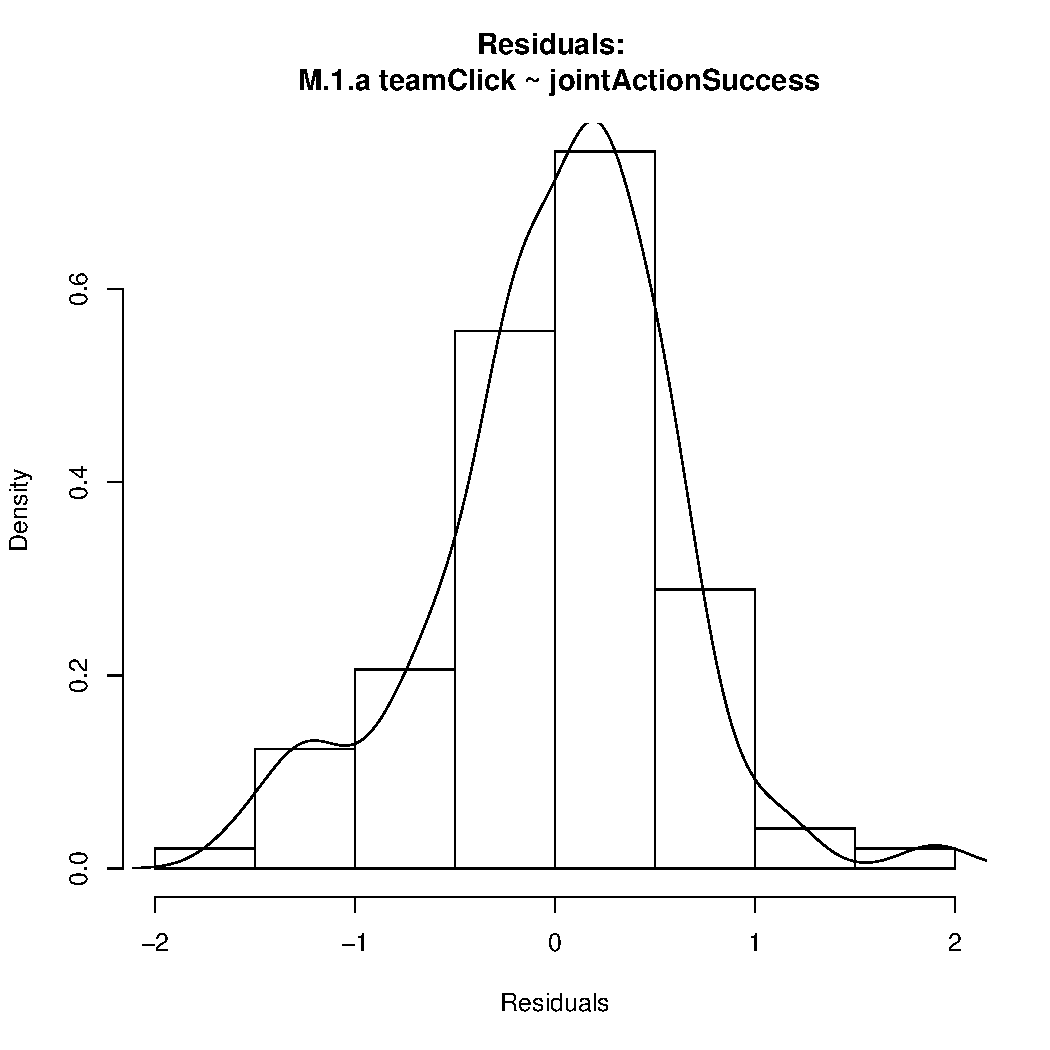
\includegraphics[scale =.4]{images/MLM1aHist.pdf}
     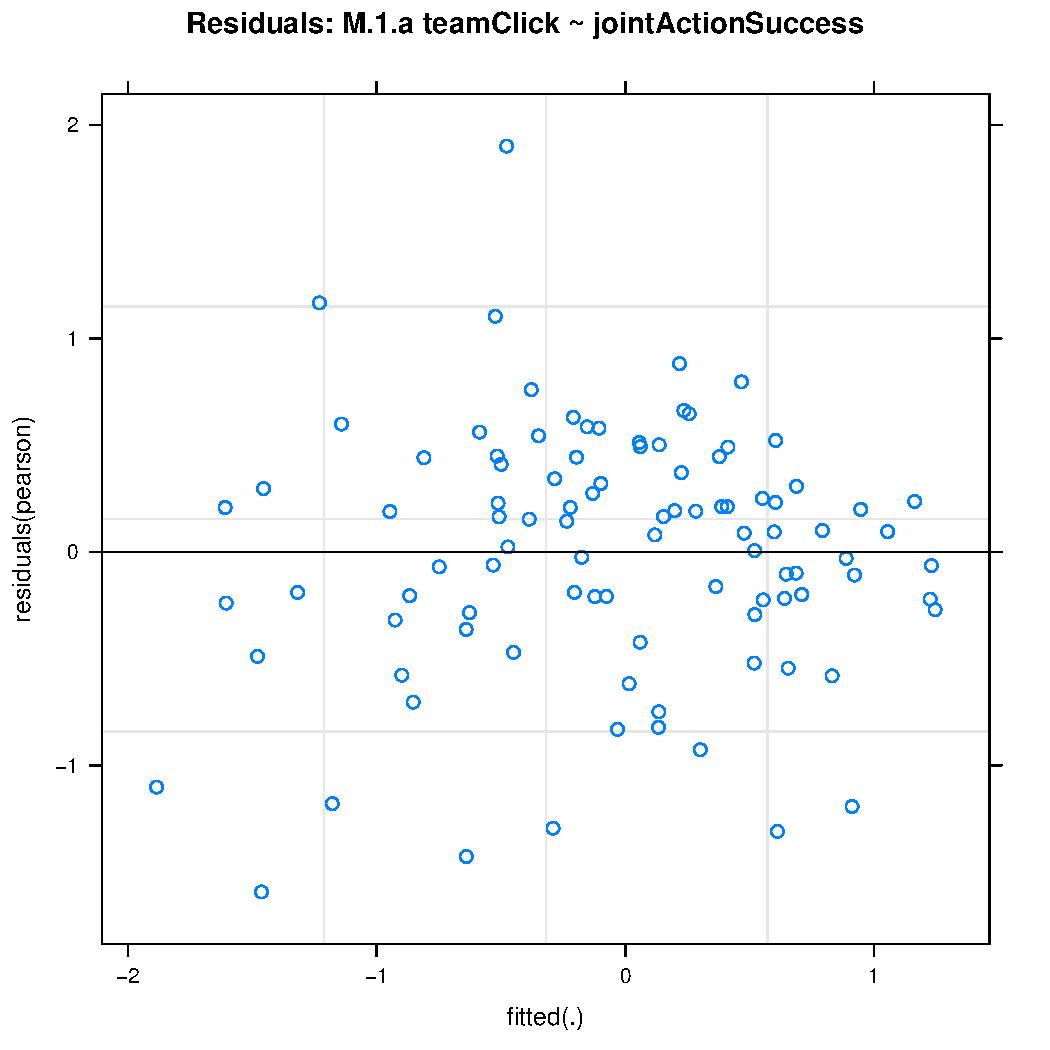
\includegraphics[scale =.4]{images/MLM1aScatter.pdf}
     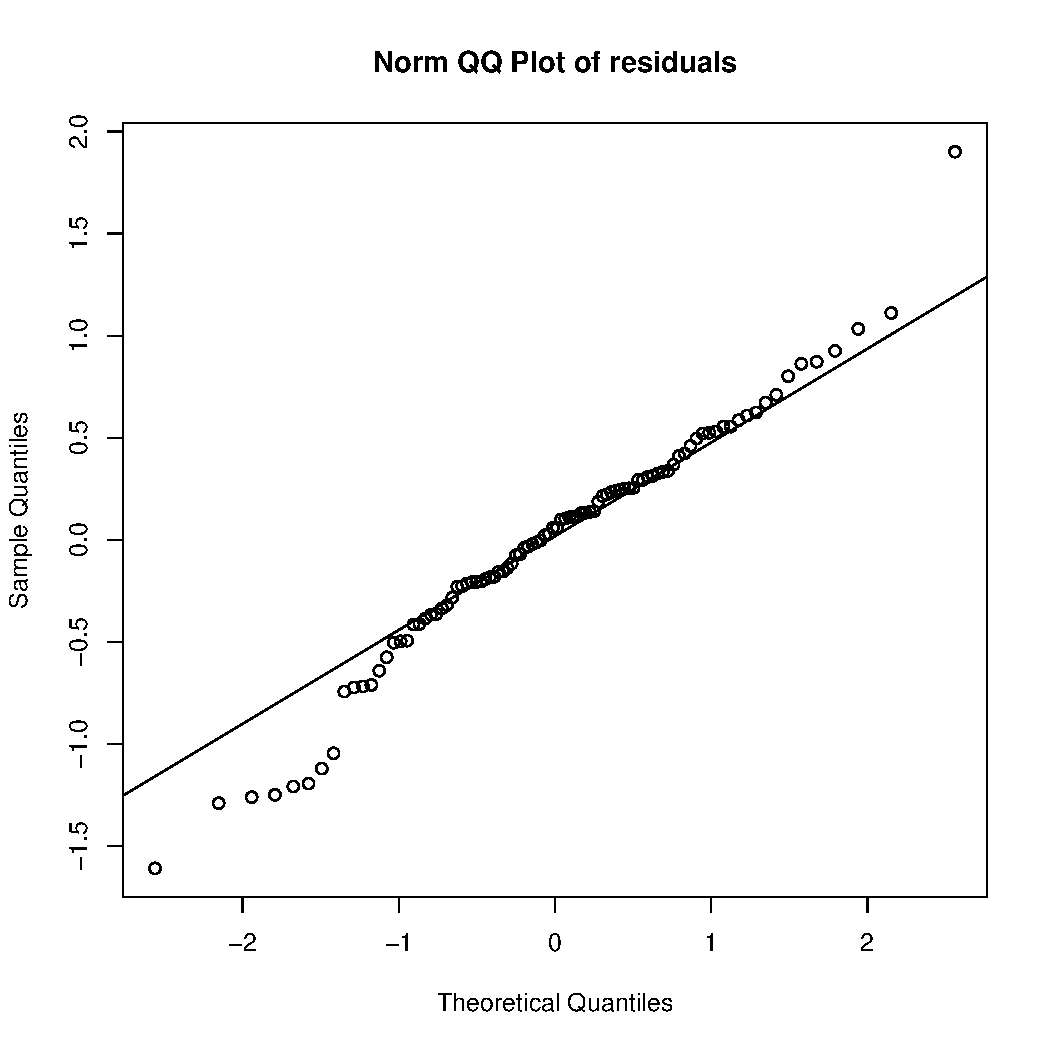
\includegraphics[scale =.4]{images/MLM1aQQPlot.pdf}
     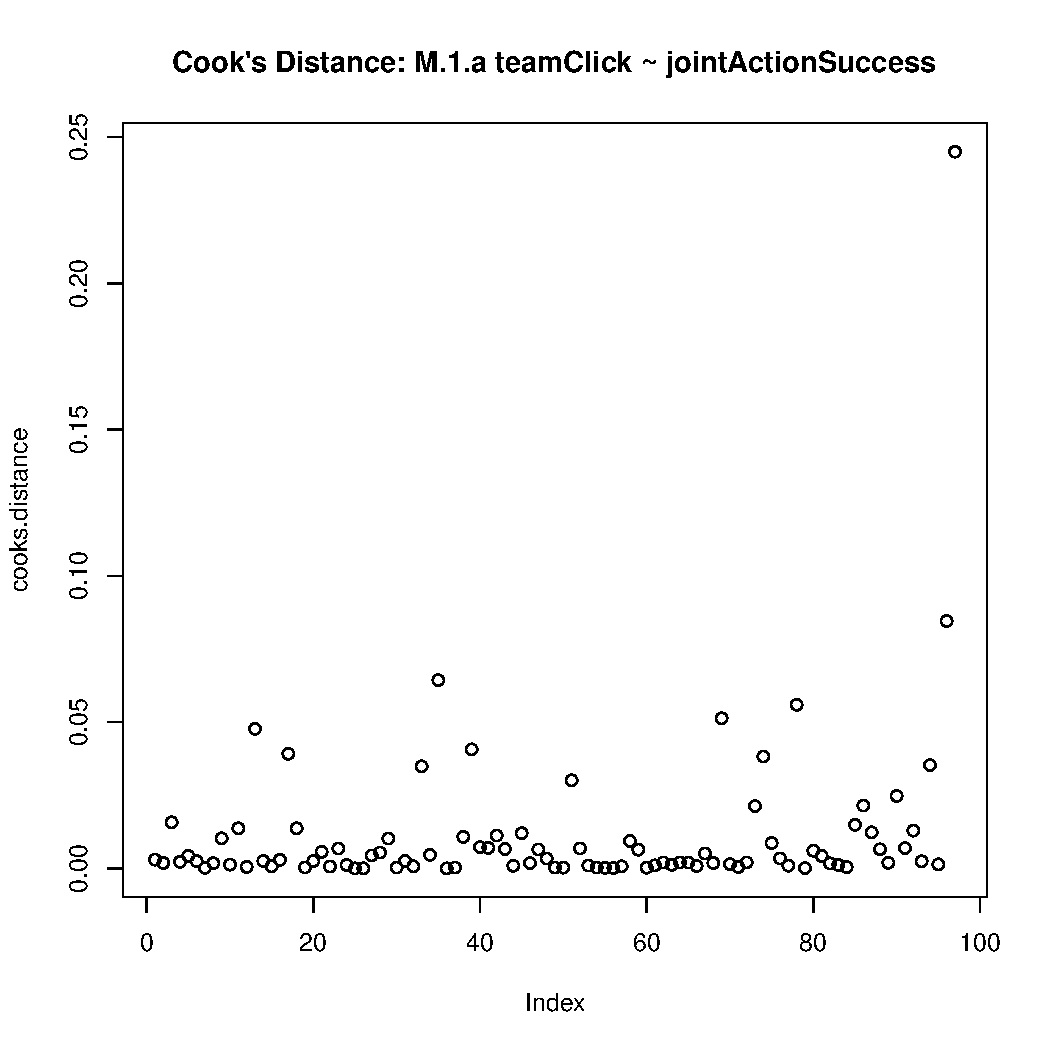
\includegraphics[scale =.4]{images/MLM1aCooksD.pdf}
     \caption{Model assumptions: 1.a Team Performance Components Predicts Team Click}
     \label{fig:MLM1aAssumptions}
 \end{figure}



 \subsubsection{Pre- to Post Tournament}

 
\begin{table}
\begin{center}
\begin{tabular}{l c c c }
\toprule
 & Intercept & Main effect & Controls \\
\midrule
(constant)                                               & $0.10$   & $0.10$                & $0.01$                \\
                                                         & $(0.13)$ & $(0.08)$              & $(0.40)$              \\
Team Performance Components Change                       &          & $\mathbf{0.47}^{***}$ & $\mathbf{0.51}^{***}$ \\
                                                         &          & $(0.08)$              & $(0.11)$              \\
Ind Performance Components Change                        &          &                       & $-0.00$               \\
                                                         &          &                       & $(0.10)$              \\
Objective Competence                                     &          &                       & $0.02$                \\
                                                         &          &                       & $(0.10)$              \\
Subjective Competence                                    &          &                       & $-0.01$               \\
                                                         &          &                       & $(0.08)$              \\
Final Rank                                               &          &                       & $-0.03$               \\
                                                         &          &                       & $(0.04)$              \\
Minutes Total                                            &          &                       & $0.01$                \\
                                                         &          &                       & $(0.00)$              \\
Points Total                                             &          &                       & $0.01$                \\
                                                         &          &                       & $(0.01)$              \\
Fatigue                                                  &          &                       & $-0.12$               \\
                                                         &          &                       & $(0.09)$              \\
Extraverted                                              &          &                       & $-0.01$               \\
                                                         &          &                       & $(0.05)$              \\
\midrule
AIC                                                      & 267.19   & 227.50                & 218.66                \\
BIC                                                      & 274.97   & 243.07                & 253.66                \\
Log Likelihood                                           & -130.59  & -107.75               & -95.33                \\
Num. obs.                                                & 99       & 99                    & 90                    \\
Num. groups: team                                        & 14       & 14                    & 13                    \\

\bottomrule
\multicolumn{4}{l}{\scriptsize{Coefficients with $p < 0.05$ in \textbf{bold}. Marginal $R^2 = .40$, Conditional $R^2 = .47$}}
\end{tabular}
\caption{Prediction 1: Team Performance Components Change predicts Team Click Change in the Pre- to Post-Tournament survey data (n = 90).}
\label{tab:MLM21aJointActionSuccessClick}
\end{center}
\end{table}


 \begin{figure}[htbp]
   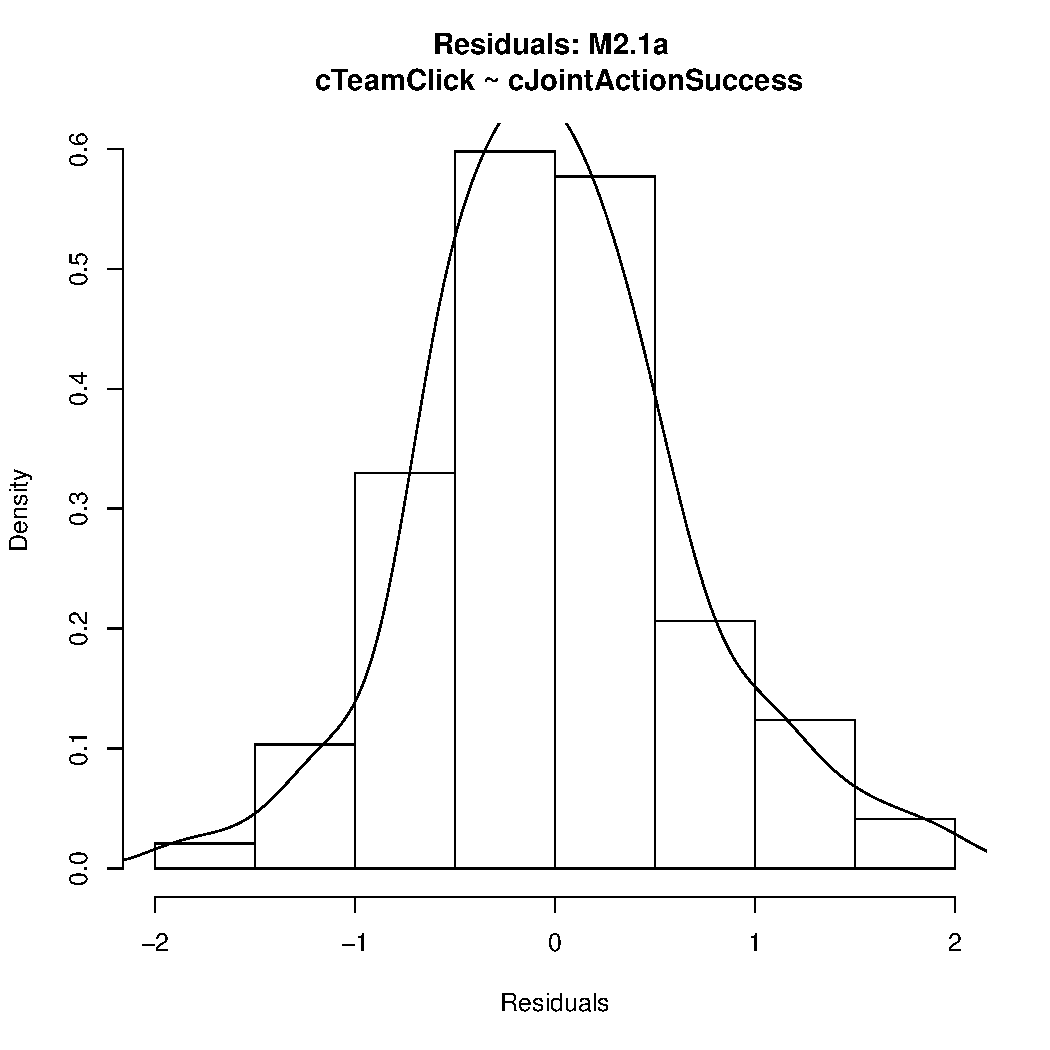
\includegraphics[scale =.4]{images/MLM21aHist.pdf}
   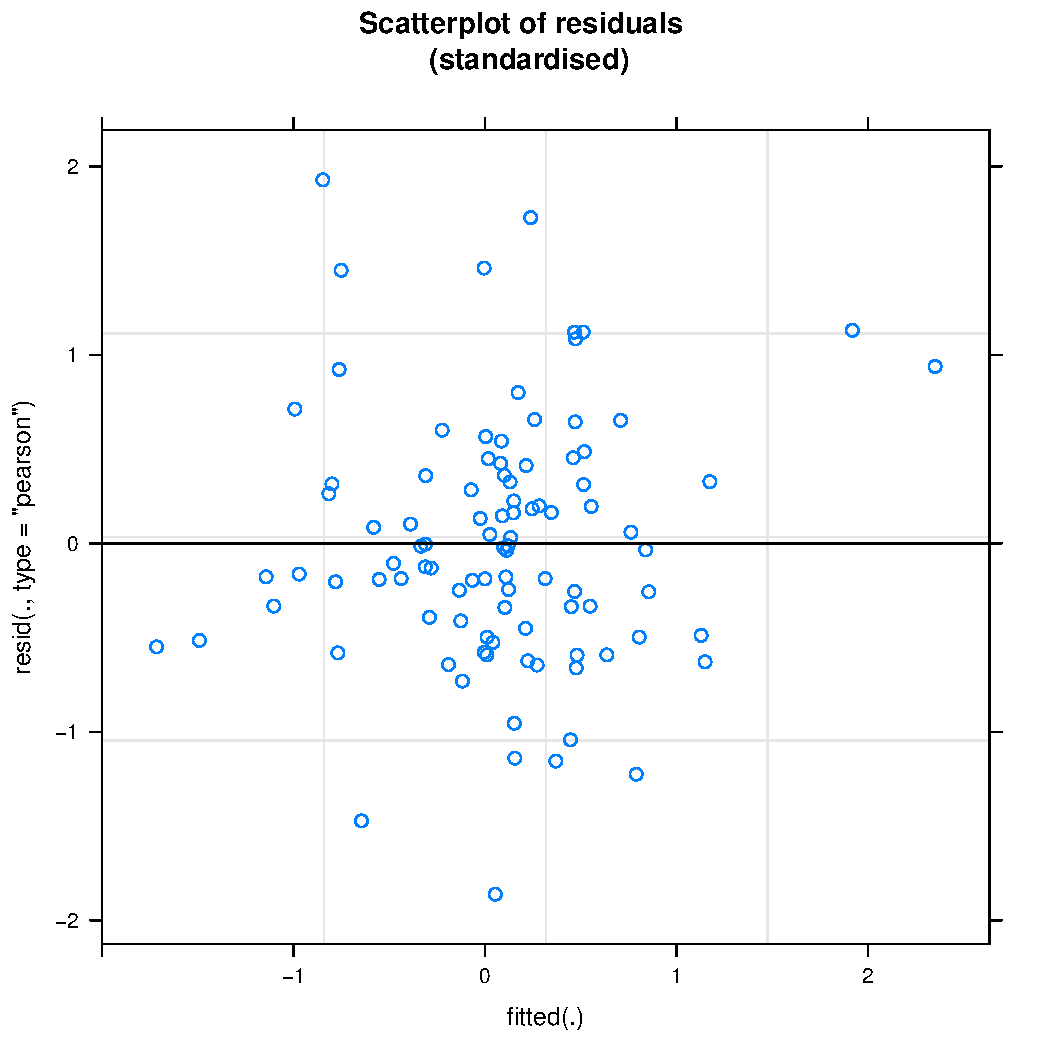
\includegraphics[scale =.4]{images/MLM21aScatter.pdf}
   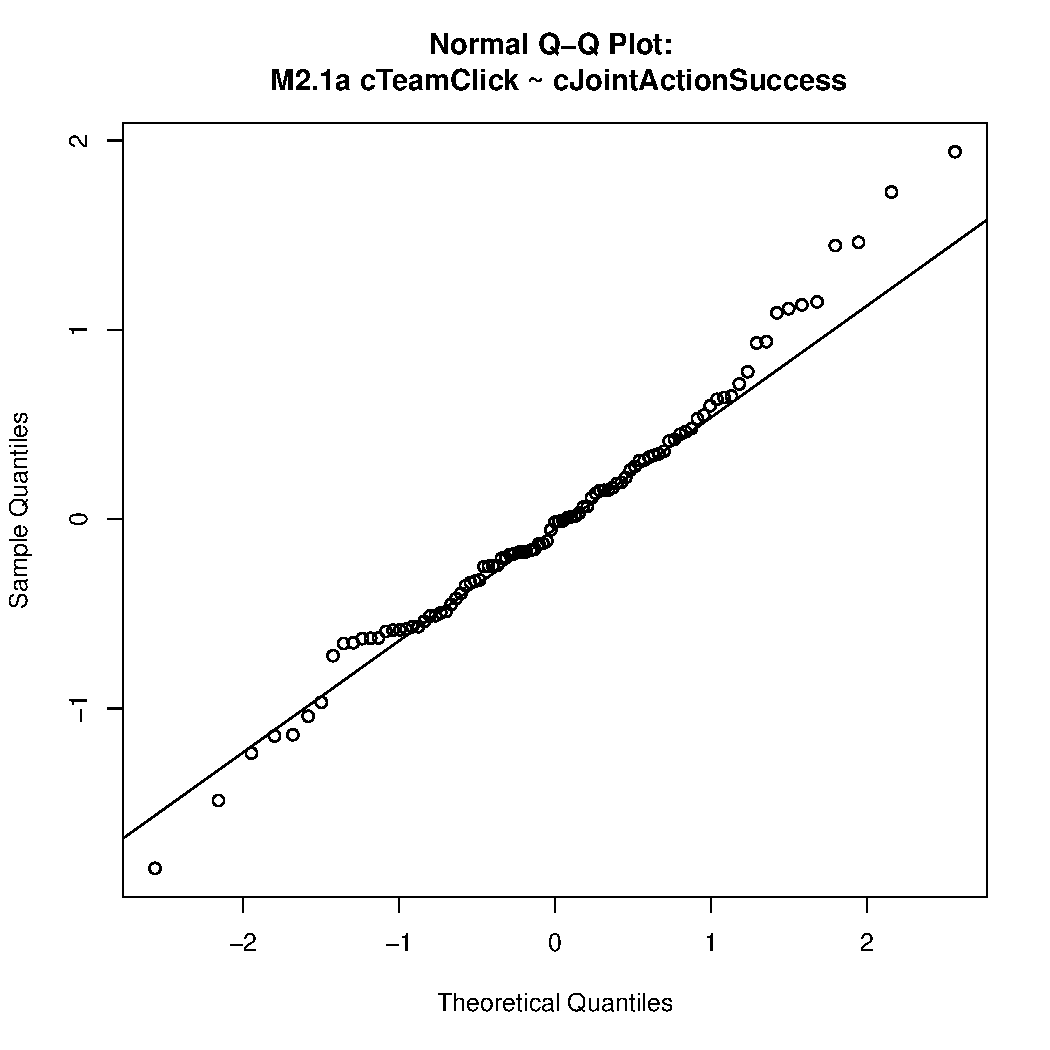
\includegraphics[scale =.4]{images/MLM21aQQNorm.pdf}
   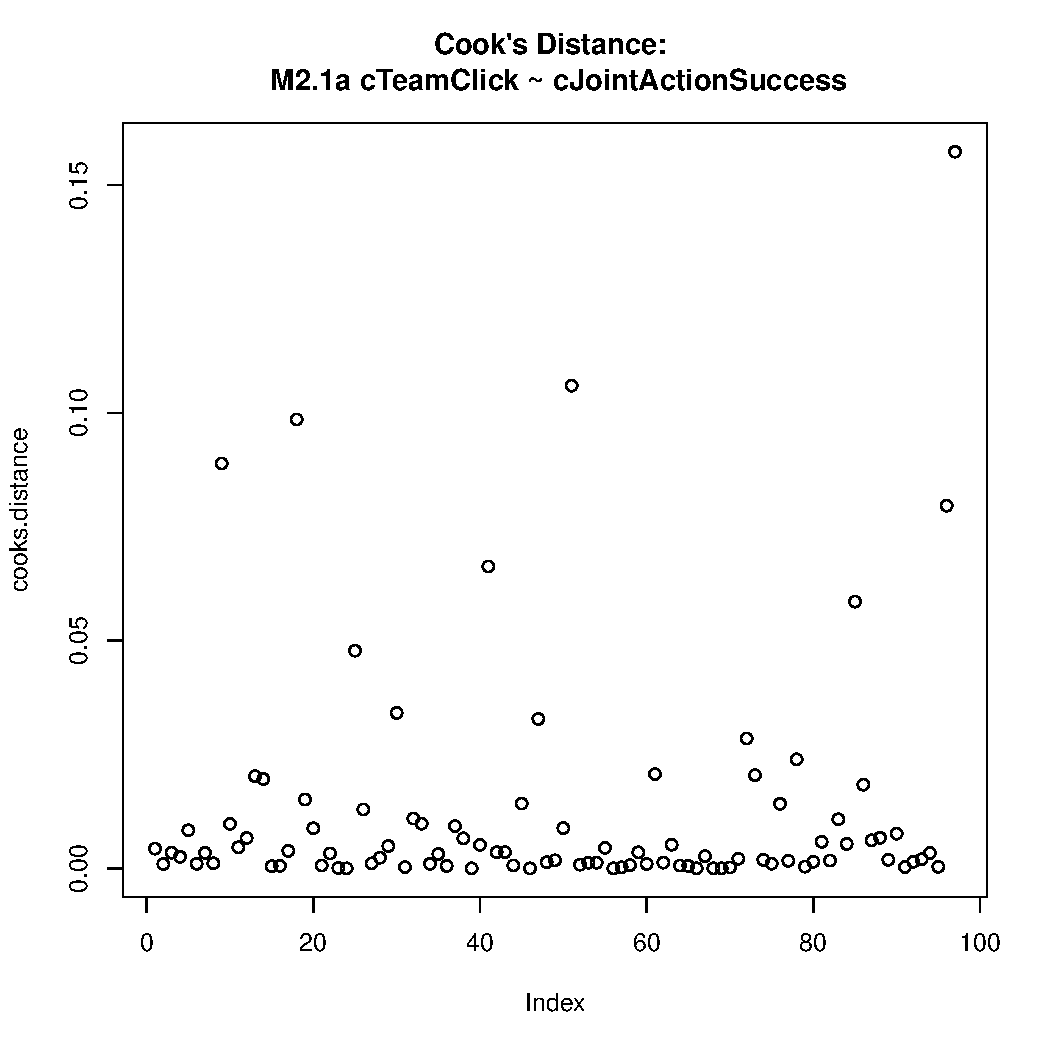
\includegraphics[scale =.4]{images/MLM21aCooksD.pdf}
   \caption{Model assumptions: Team Performance Components Change Team Click Change}
   \label{fig:MLM21aAssumptions}
 \end{figure}


 %\subsubsection{Overall Tournament}
 %\myparagraph{Model comparisons}
 %\myparagraph{Model robustness checks}



  \subsection{Prediction 2: Team Click predicts Social Bonding \label{app8:MLM2}}

       \subsubsection{Post-Tournament\label{app8:MLM2a}}


            %\begin{align*}
    %     Social Bonding  \end{align*}% = Team Click\\
                              %+ Objective Competence + %Subjective Competence  \\
                               %+ Tournament performance %measures \\
            %\end{align*}


        
% Table created by stargazer v.5.2 by Marek Hlavac, Harvard University. E-mail: hlavac at fas.harvard.edu
% Date and time: Mon, Jun 26, 2017 - 20:48:41
\begin{table}[!htbp] \centering 
  \caption{socialBonding = teamClick} 
  \label{tab:MLM2aTeamClickBonding} 
\begin{tabular}{@{\extracolsep{5pt}}lccc} 
\\[-1.8ex]\hline 
\hline \\[-1.8ex] 
 & \multicolumn{3}{c}{\textit{Dependent variable:}} \\ 
\cline{2-4} 
\\[-1.8ex] & \multicolumn{3}{c}{socialBonding} \\ 
\\[-1.8ex] & (1) & (2) & (3)\\ 
\hline \\[-1.8ex] 
 (constant) & $-$0.01 & $-$0.0002 & 0.21 \\ 
  & (0.10) & (0.07) & (0.27) \\ 
  & & & \\ 
 teamClick &  & 0.64$^{***}$ & 0.67$^{***}$ \\ 
  &  & (0.08) & (0.08) \\ 
  & & & \\ 
 objectiveCompetence &  &  & 0.04 \\ 
  &  &  & (0.08) \\ 
  & & & \\ 
 subjectiveCompetence &  &  & 0.12 \\ 
  &  &  & (0.07) \\ 
  & & & \\ 
 finalRank &  &  & $-$0.01 \\ 
  &  &  & (0.04) \\ 
  & & & \\ 
 minutesTotal &  &  & $-$0.003 \\ 
  &  &  & (0.004) \\ 
  & & & \\ 
 pointsTotal &  &  & $-$0.002 \\ 
  &  &  & (0.01) \\ 
  & & & \\ 
\hline \\[-1.8ex] 
Marginal R-squared &  &  & .49 \\ 
Conditional R-squared &  &  & .51 \\ 
Observations & 118 & 118 & 97 \\ 
Log Likelihood & $-$151.95 & $-$118.76 & $-$97.75 \\ 
Akaike Inf. Crit. & 309.90 & 249.53 & 217.50 \\ 
Bayesian Inf. Crit. & 318.21 & 266.15 & 245.82 \\ 
\hline 
\hline \\[-1.8ex] 
\textit{Note:}  & \multicolumn{3}{r}{$^{*}$p$<$0.05; $^{**}$p$<$0.01; $^{***}$p$<$0.001} \\ 
\end{tabular} 
\end{table} 


              \begin{figure}[htbp]
                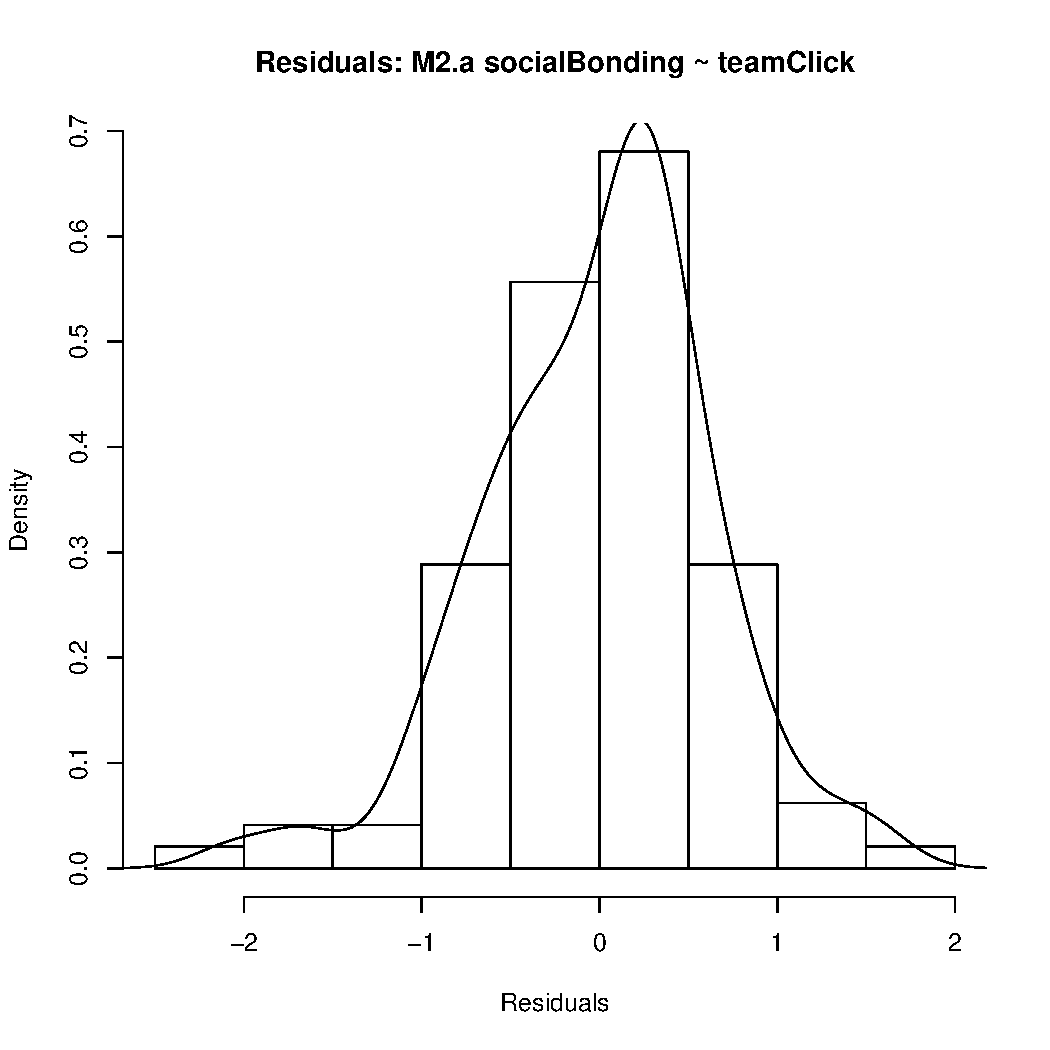
\includegraphics[scale =.4]{images/MLM2aHist.pdf}
                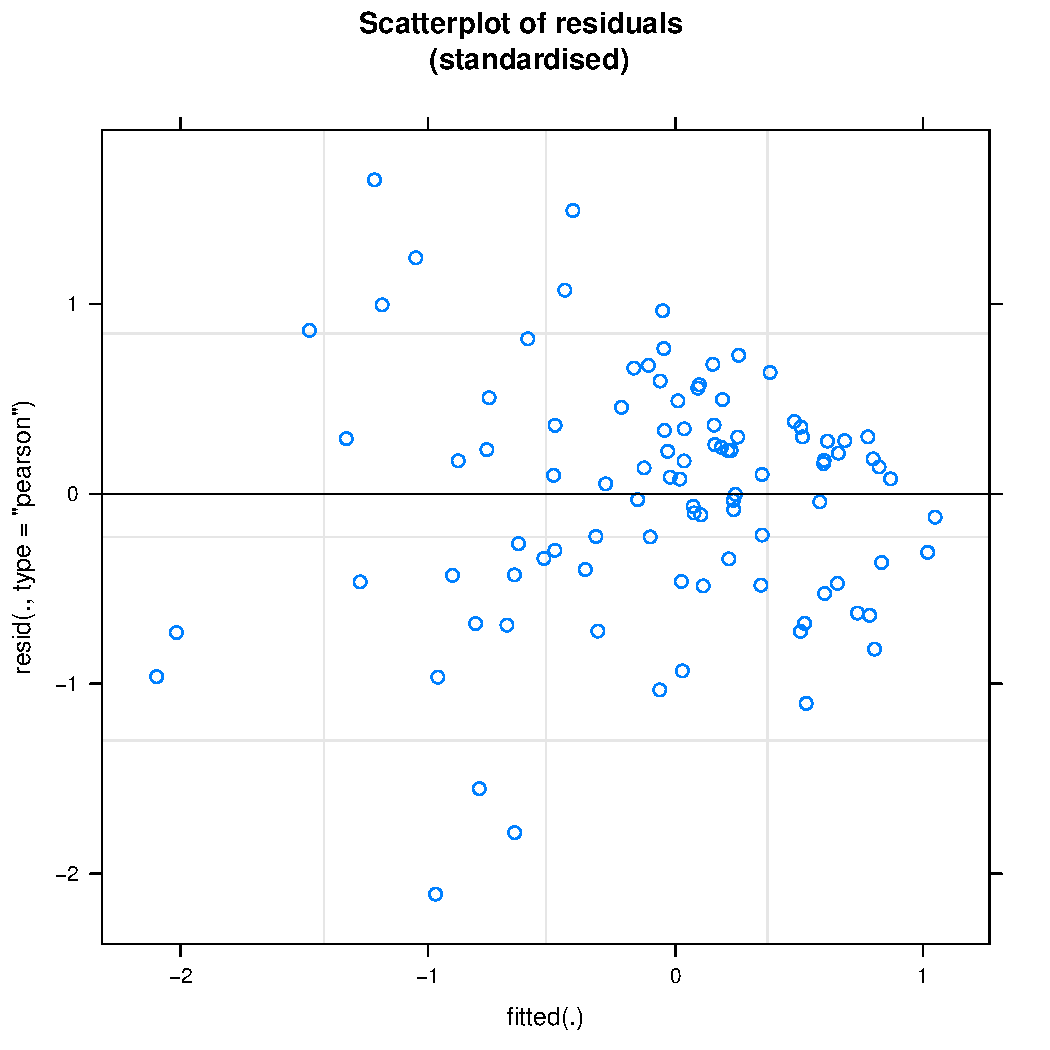
\includegraphics[scale =.4]{images/MLM2aScatter.pdf}
                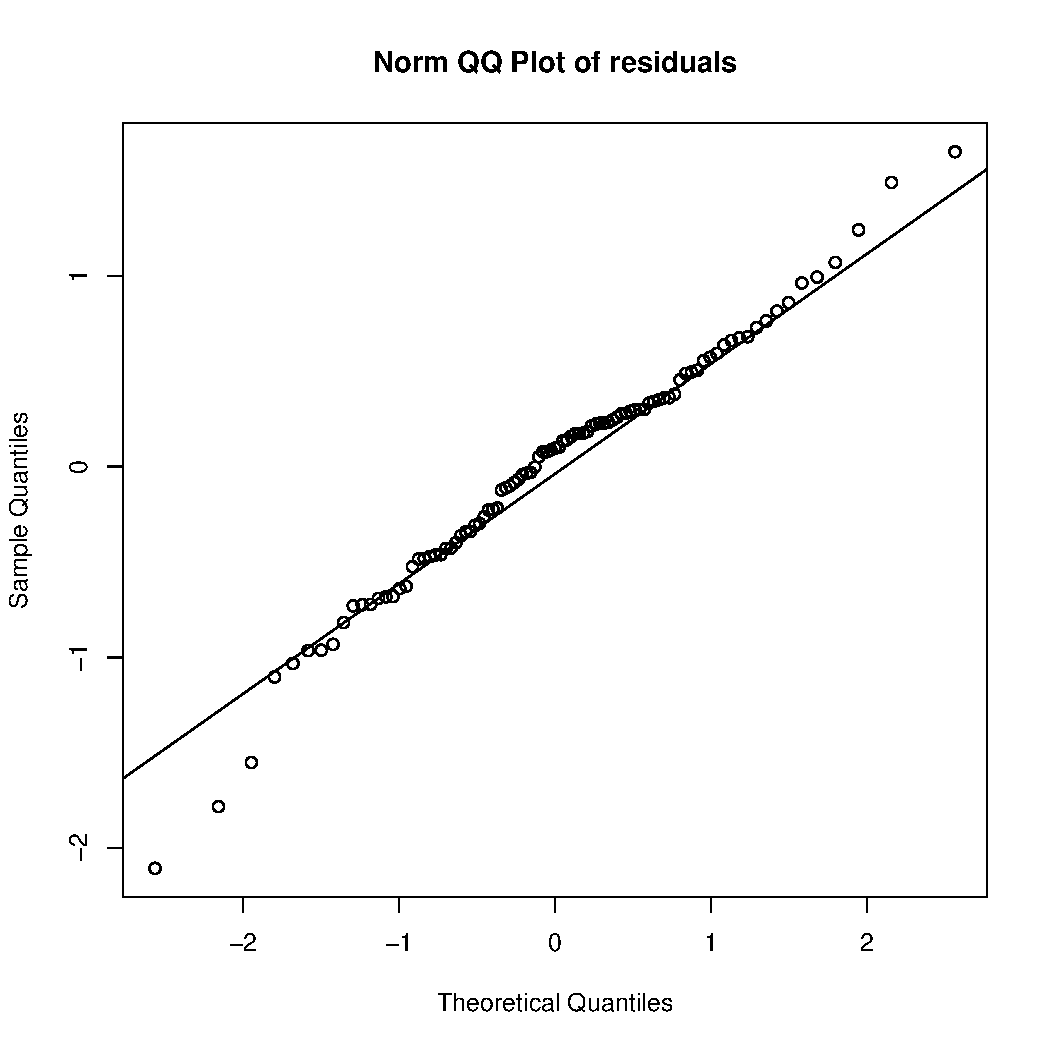
\includegraphics[scale =.4]{images/MLM2aQQNorm.pdf}
                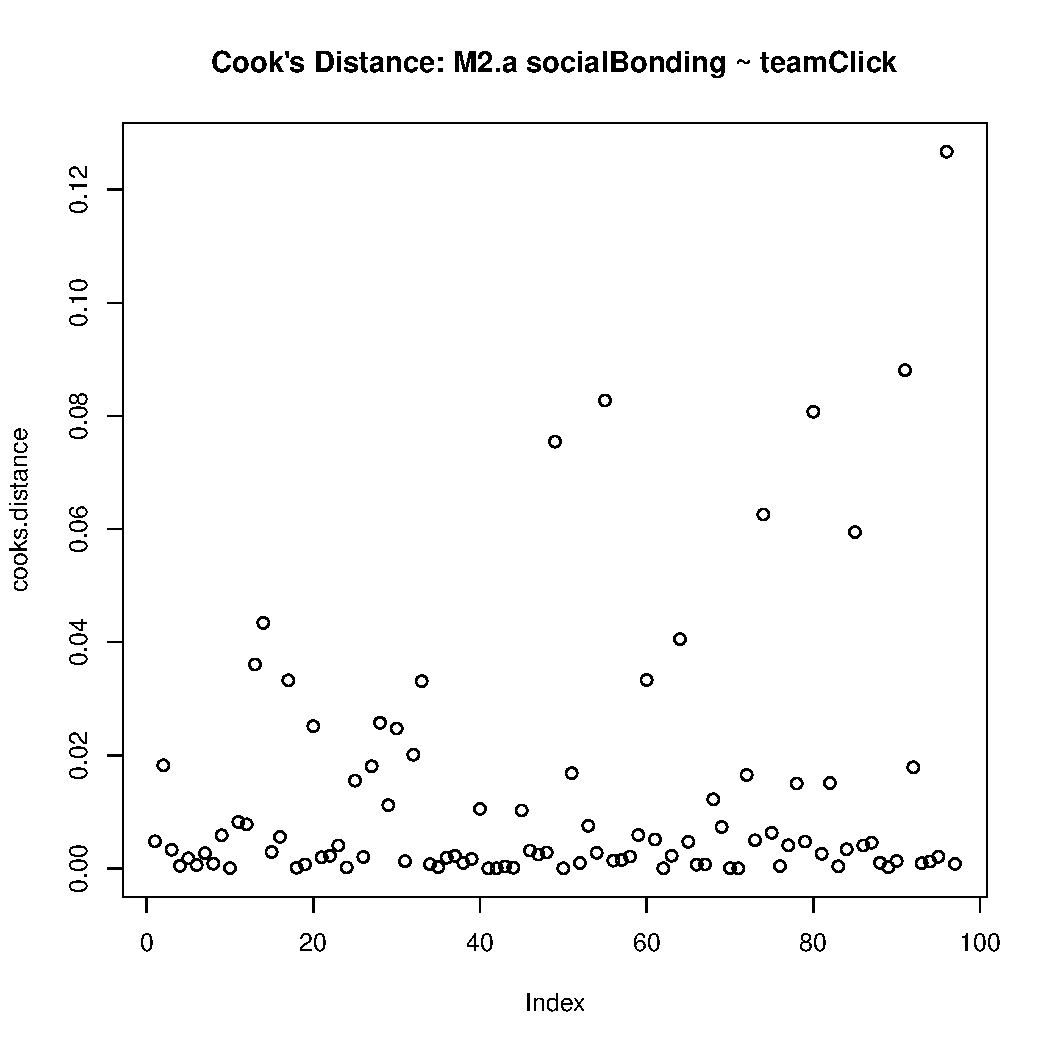
\includegraphics[scale =.4]{images/MLM2aCooksD.pdf}
                \caption{Model assumptions: M2a Team Click predicts Social Bonding}
                \label{fig:MLM2aAssumptions}
              \end{figure}




      \subsubsection{Pre- to Post Tournament}


      
\begin{table}
\begin{center}
\begin{tabular}{l c c c }
\toprule
 & Intercept & Main effect & Controls \\
\midrule
(constant)                                     & $\mathbf{0.34}^{***}$ & $\mathbf{0.31}^{***}$ & $0.29$               \\
                                               & $(0.09)$              & $(0.08)$              & $(0.46)$             \\
Team Click Change                              &                       & $\mathbf{0.39}^{***}$ & $\mathbf{0.37}^{**}$ \\
                                               &                       & $(0.11)$              & $(0.14)$             \\
Objective Competence                           &                       &                       & $0.08$               \\
                                               &                       &                       & $(0.10)$             \\
Subjective Competence                          &                       &                       & $0.01$               \\
                                               &                       &                       & $(0.09)$             \\
Final Rank                                     &                       &                       & $0.00$               \\
                                               &                       &                       & $(0.05)$             \\
Minutes Total                                  &                       &                       & $0.01$               \\
                                               &                       &                       & $(0.00)$             \\
Points Total                                   &                       &                       & $0.00$               \\
                                               &                       &                       & $(0.01)$             \\
Fatigue                                        &                       &                       & $-0.09$              \\
                                               &                       &                       & $(0.10)$             \\
Extraverted                                    &                       &                       & $-0.03$              \\
                                               &                       &                       & $(0.06)$             \\
\midrule
AIC                                            & 265.55                & 256.54                & 241.81               \\
BIC                                            & 273.34                & 272.11                & 274.31               \\
Log Likelihood                                 & -129.78               & -122.27               & -107.90              \\
Num. obs.                                      & 99                    & 99                    & 90                   \\
Num. groups: team                              & 14                    & 14                    & 13                   \\
\bottomrule
\multicolumn{4}{l}{\scriptsize{Coefficients with $p < 0.05$ in \textbf{bold}. Marginal $R^2 = .17$, Conditional $R^2 = .23$}}
\end{tabular}
\caption{Prediction 2: Team Click Change predicts Social Bonding Change in the Post-Tournament survey data (n = 90).}
\label{tab:MLM22acClickcBonding}
\end{center}
\end{table}


      \begin{figure}[htbp]
        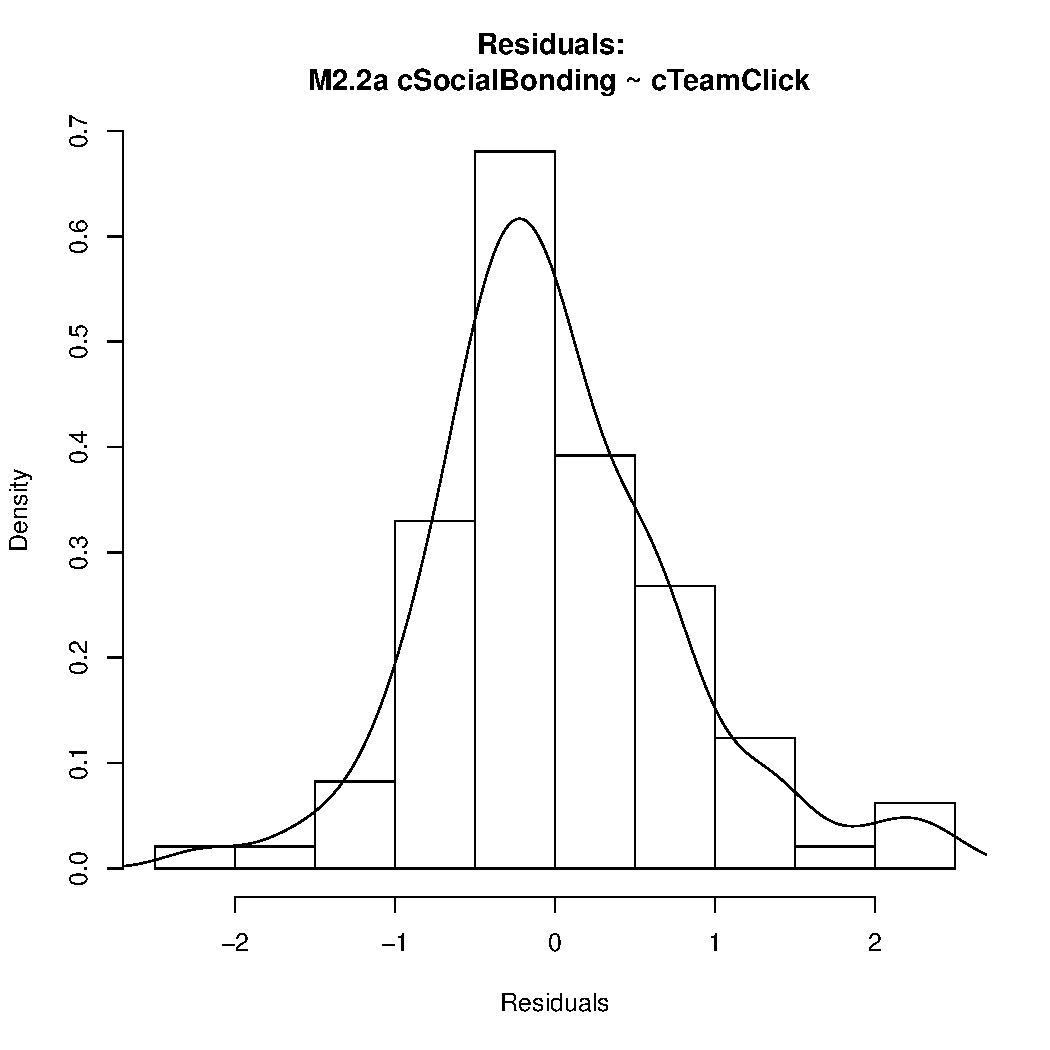
\includegraphics[scale =.4]{images/MLM22aHist.pdf}
        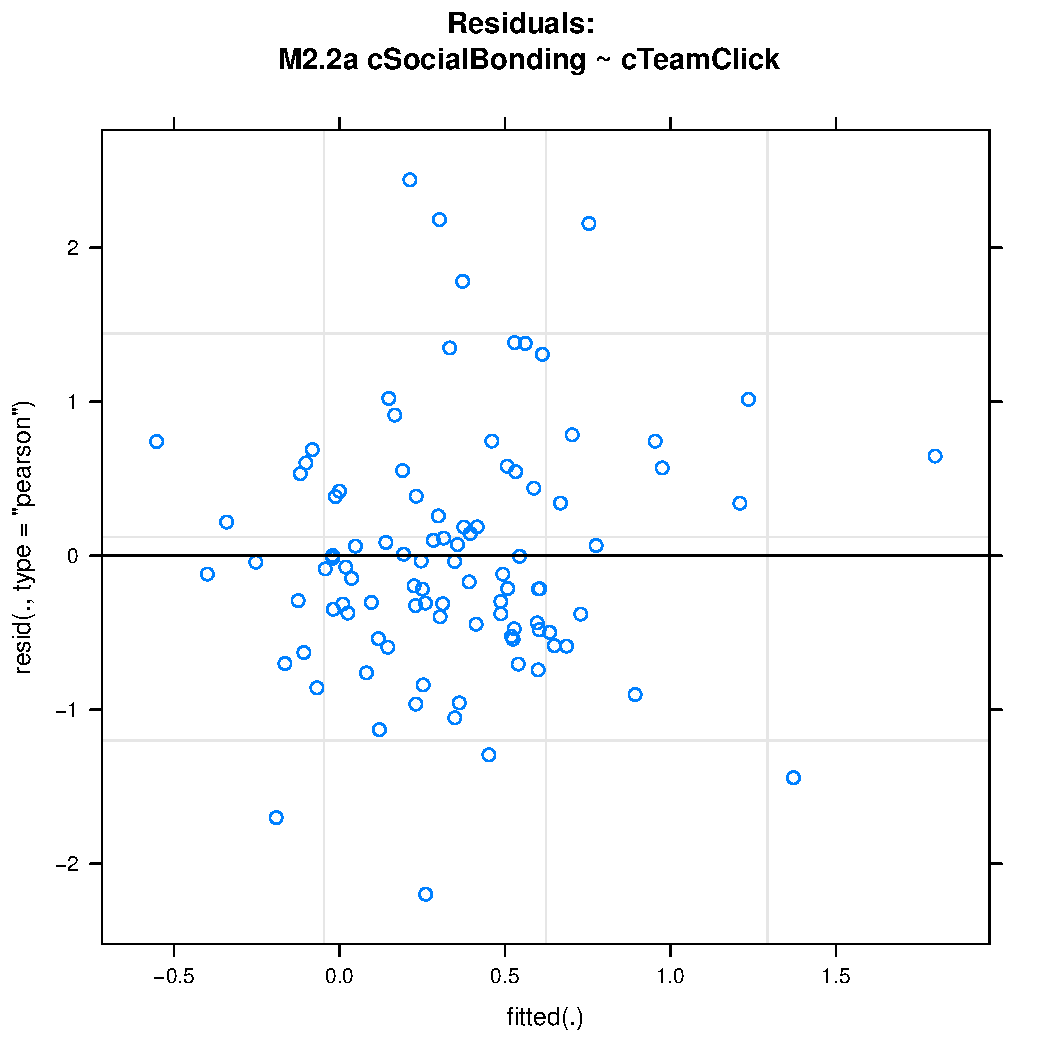
\includegraphics[scale =.4]{images/MLM22aScatter.pdf}
        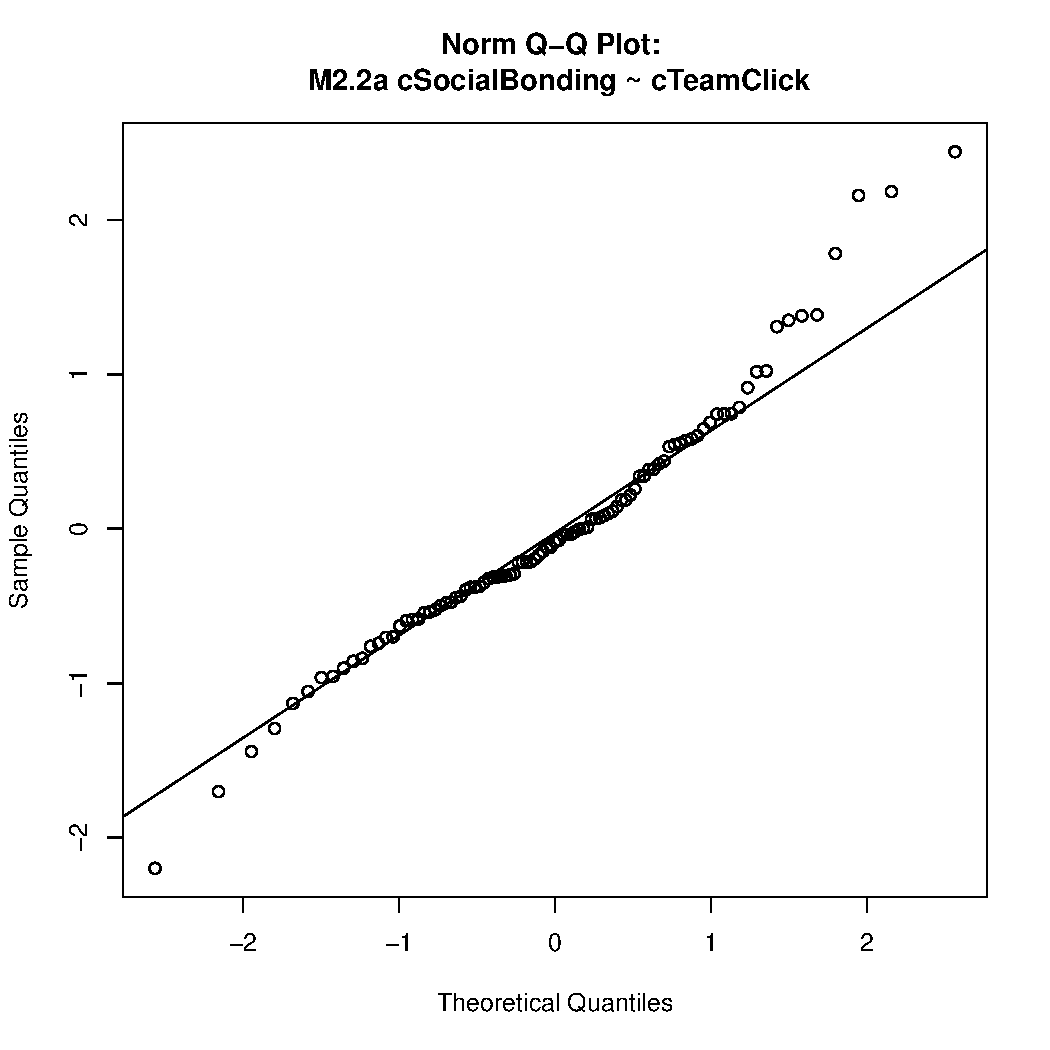
\includegraphics[scale =.4]{images/MLM22aQQNorm.pdf}
        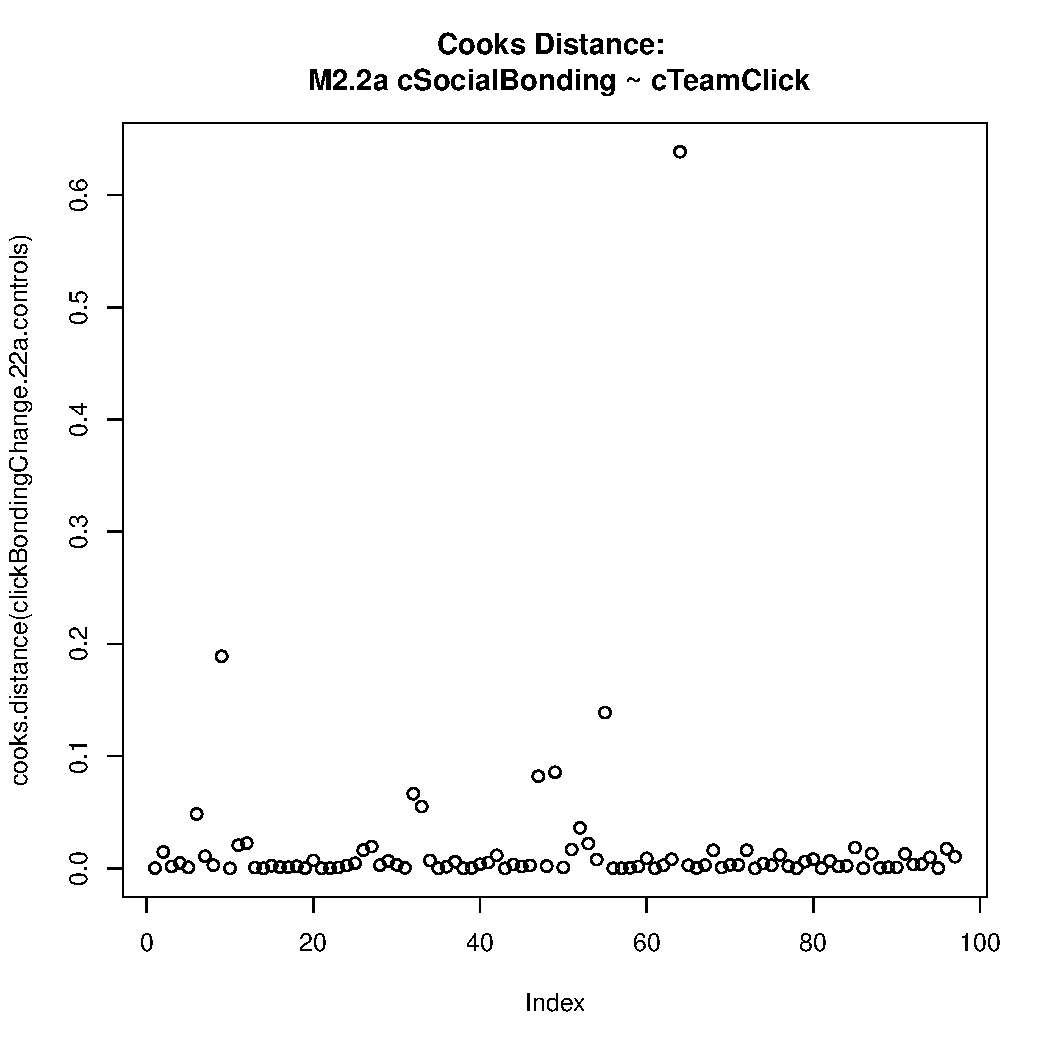
\includegraphics[scale =.4]{images/MLM22aCooksD.pdf}
        \caption{Model assumptions: M2.2a Change in Team Click predicts change in Social Bonding}
        \label{fig:MLM22aAssumptions}
      \end{figure}





      \subsubsection{Overall Tournament\label{app8:MLM32a}}


        %
% Table created by stargazer v.5.2 by Marek Hlavac, Harvard University. E-mail: hlavac at fas.harvard.edu
% Date and time: Thu, Sep 14, 2017 - 09:39:55
\begin{table}[!htbp] \centering 
  \caption{bondingTournament ~ teamClickTournament} 
  \label{tab:MLM31bclickBondingTournament} 
\footnotesize 
\begin{tabular}{@{\extracolsep{5pt}}lccc} 
\\[-1.8ex]\hline 
\hline \\[-1.8ex] 
 & \multicolumn{3}{c}{\textit{Dependent variable:}} \\ 
\cline{2-4} 
\\[-1.8ex] & (1) & (2) & (3)\\ 
\hline \\[-1.8ex] 
 (constant) & $-$0.00 & $-$1.46$^{***}$ & $-$1.59$^{***}$ \\ 
  & (0.04) & (0.08) & (0.15) \\ 
  & & & \\ 
 teamPerformanceExpectations &  & 0.02$^{***}$ & 0.02$^{***}$ \\ 
  &  & (0.001) & (0.001) \\ 
  & & & \\ 
 indPerformanceExpectations &  &  & 0.004$^{**}$ \\ 
  &  &  & (0.002) \\ 
  & & & \\ 
 objectiveCompetence &  &  & 0.02 \\ 
  &  &  & (0.04) \\ 
  & & & \\ 
 subjectiveCompetence &  &  & 0.08$^{*}$ \\ 
  &  &  & (0.04) \\ 
  & & & \\ 
 finalRank &  &  & $-$0.0002 \\ 
  &  &  & (0.02) \\ 
  & & & \\ 
 minutesTotal &  &  & $-$0.001 \\ 
  &  &  & (0.002) \\ 
  & & & \\ 
 pointsTotal &  &  & 0.003 \\ 
  &  &  & (0.003) \\ 
  & & & \\ 
\hline \\[-1.8ex] 
Marginal R-squared & .47 & .49 &  \\ 
Conditional R-squared & .66 & .66 &  \\ 
Observations & 564 & 444 & 331 \\ 
Log Likelihood & $-$772.35 & $-$412.33 & $-$303.82 \\ 
Akaike Inf. Crit. & 1,552.70 & 842.67 & 637.65 \\ 
Bayesian Inf. Crit. & 1,570.04 & 879.53 & 694.68 \\ 
\hline 
\hline \\[-1.8ex] 
\textit{Note:}  & \multicolumn{3}{r}{$^{*}$p$<$0.05; $^{**}$p$<$0.01; $^{***}$p$<$0.001} \\ 
\end{tabular} 
\end{table} 


        %
% Table created by stargazer v.5.2 by Marek Hlavac, Harvard University. E-mail: hlavac at fas.harvard.edu
% Date and time: Thu, Sep 14, 2017 - 09:39:58
\begin{table}[!htbp] \centering 
  \caption{Model Adjustment Comparison:bondingTournament ~ teamClickTournament} 
  \label{MLM31bclickBondingTournamentModelComparison} 
\tiny 
\begin{tabular}{@{\extracolsep{5pt}}lcccc} 
\\[-1.8ex]\hline 
\hline \\[-1.8ex] 
 & \multicolumn{4}{c}{\textit{Dependent variable:}} \\ 
\cline{2-5} 
 & model & log-transformed & outliers removed & outliers + log-transformed \\ 
\\[-1.8ex] & (1) & (2) & (3) & (4)\\ 
\hline \\[-1.8ex] 
 (constant) & $-$1.59$^{***}$ & 1.63$^{***}$ & 0.31$^{***}$ & 1.50$^{***}$ \\ 
  & (0.15) & (0.02) & (0.08) & (0.04) \\ 
  & & & & \\ 
 teamPerformanceExpectations & 0.02$^{***}$ &  &  &  \\ 
  & (0.001) &  &  &  \\ 
  & & & & \\ 
 indPerformanceExpectations & 0.004$^{**}$ &  &  &  \\ 
  & (0.002) &  &  &  \\ 
  & & & & \\ 
 objectiveCompetence &  & 0.16$^{***}$ & 0.42$^{***}$ & 0.19$^{***}$ \\ 
  &  & (0.01) & (0.04) & (0.02) \\ 
  & & & & \\ 
 subjectiveCompetence & 0.02 & 0.01 & 0.01 & 0.01 \\ 
  & (0.04) & (0.01) & (0.03) & (0.01) \\ 
  & & & & \\ 
 finalRank & 0.08$^{*}$ & 0.01 & 0.03 & 0.02 \\ 
  & (0.04) & (0.01) & (0.02) & (0.01) \\ 
  & & & & \\ 
 minutesTotal & $-$0.0002 & $-$0.004 & $-$0.01 & $-$0.01 \\ 
  & (0.02) & (0.003) & (0.01) & (0.005) \\ 
  & & & & \\ 
 pointsTotal & $-$0.001 & $-$0.001 & $-$0.002 & $-$0.001 \\ 
  & (0.002) & (0.0004) & (0.001) & (0.001) \\ 
  & & & & \\ 
 pointsTotal & 0.003 & $-$0.001 & $-$0.001 & $-$0.001 \\ 
  & (0.003) & (0.001) & (0.002) & (0.001) \\ 
  & & & & \\ 
\hline \\[-1.8ex] 
Marginal R-squared & .49 & .50 & .23 & .23 \\ 
Conditional R-squared & .66 & .61 & .35 & .34 \\ 
Shapiro-Wilk Test (p-value) & .92(<.00000000001) & .95(<.000001) & .96(<.00001) & .98(.0002) \\ 
Observations & 331 & 449 & 405 & 405 \\ 
Log Likelihood & $-$303.82 & 225.59 & $-$241.97 & 79.71 \\ 
Akaike Inf. Crit. & 637.65 & $-$423.18 & 511.94 & $-$131.42 \\ 
Bayesian Inf. Crit. & 694.68 & $-$365.69 & 567.99 & $-$75.37 \\ 
\hline 
\hline \\[-1.8ex] 
\textit{Note:}  & \multicolumn{4}{r}{$^{*}$p$<$0.05; $^{**}$p$<$0.01; $^{***}$p$<$0.001} \\ 
\end{tabular} 
\end{table} 


            \begin{figure}[htbp]
              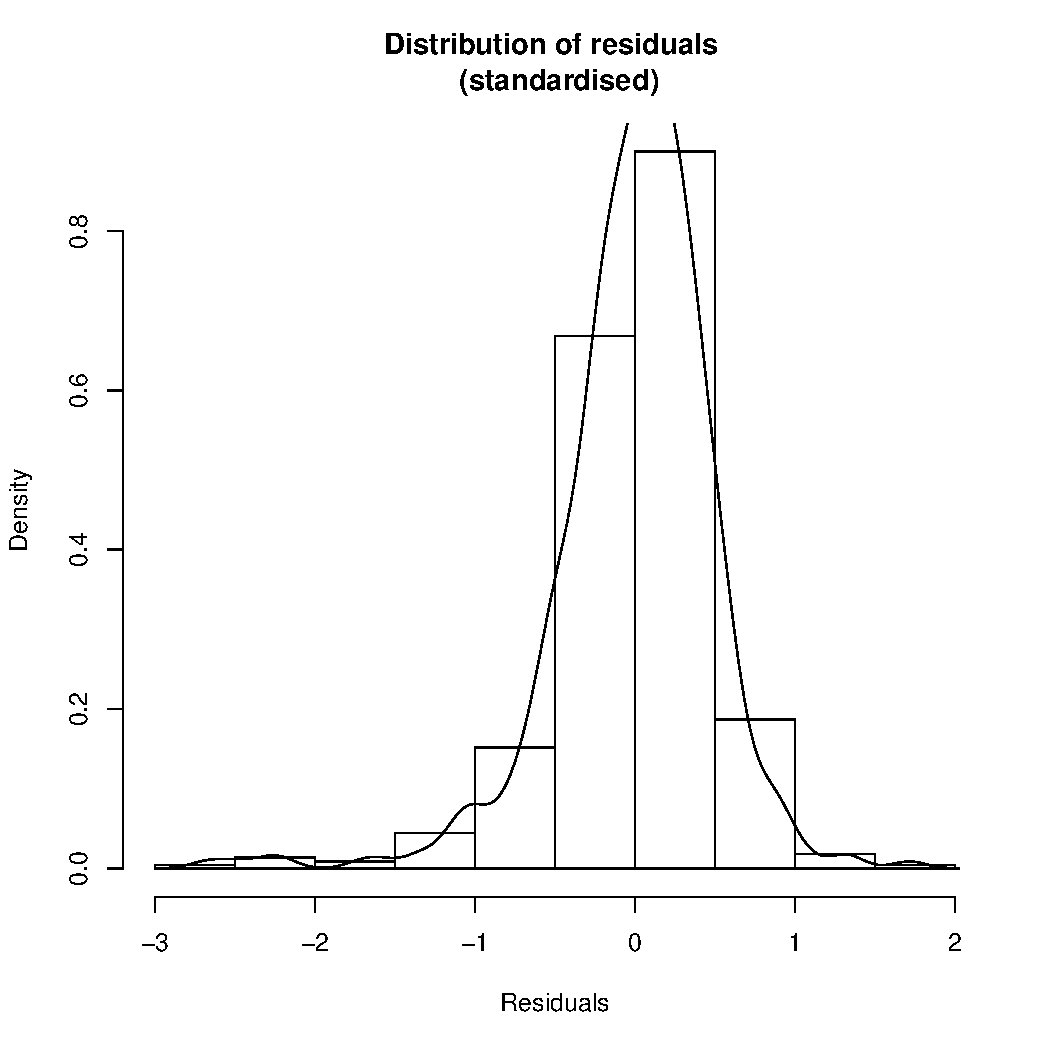
\includegraphics[scale =.4]{images/MLM31bHist.pdf}
              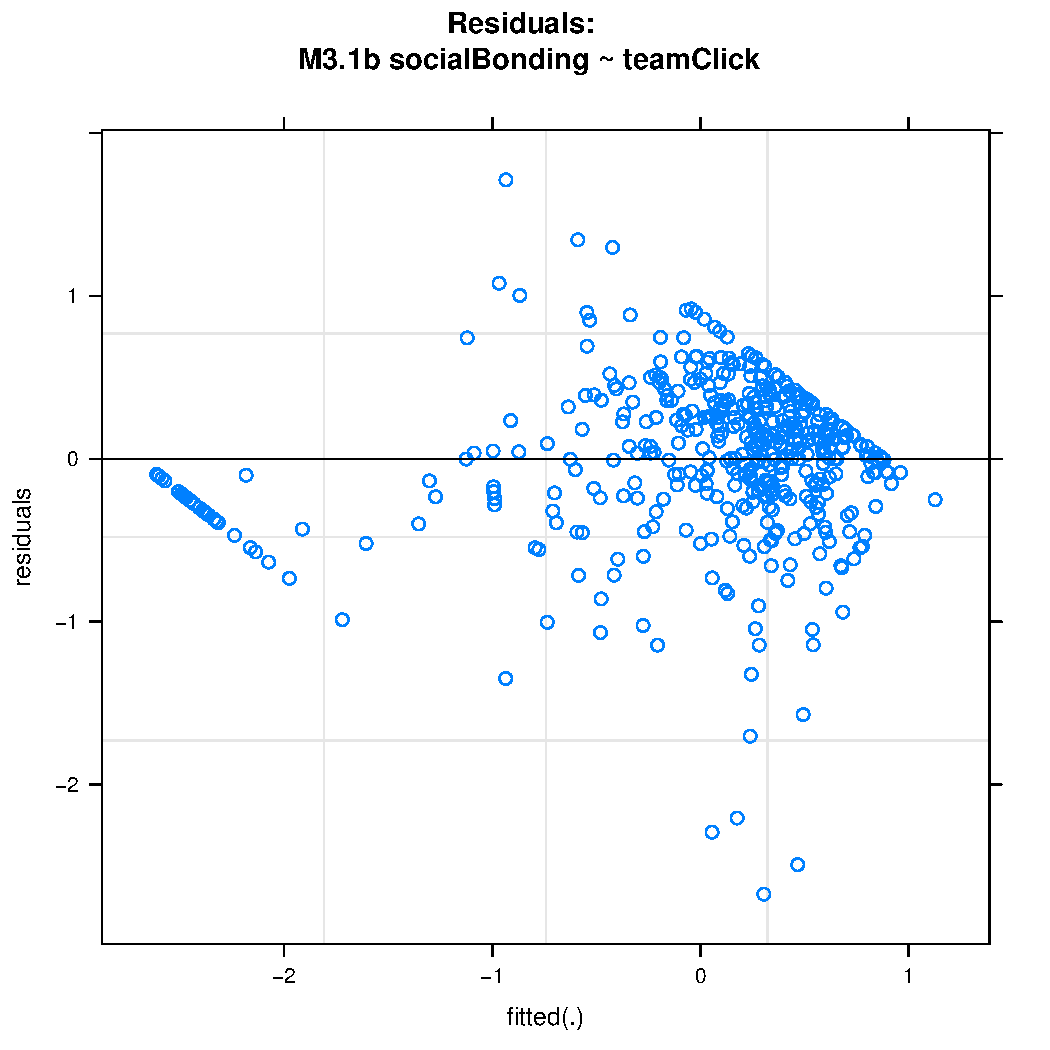
\includegraphics[scale =.4]{images/MLM31bScatter.pdf}
              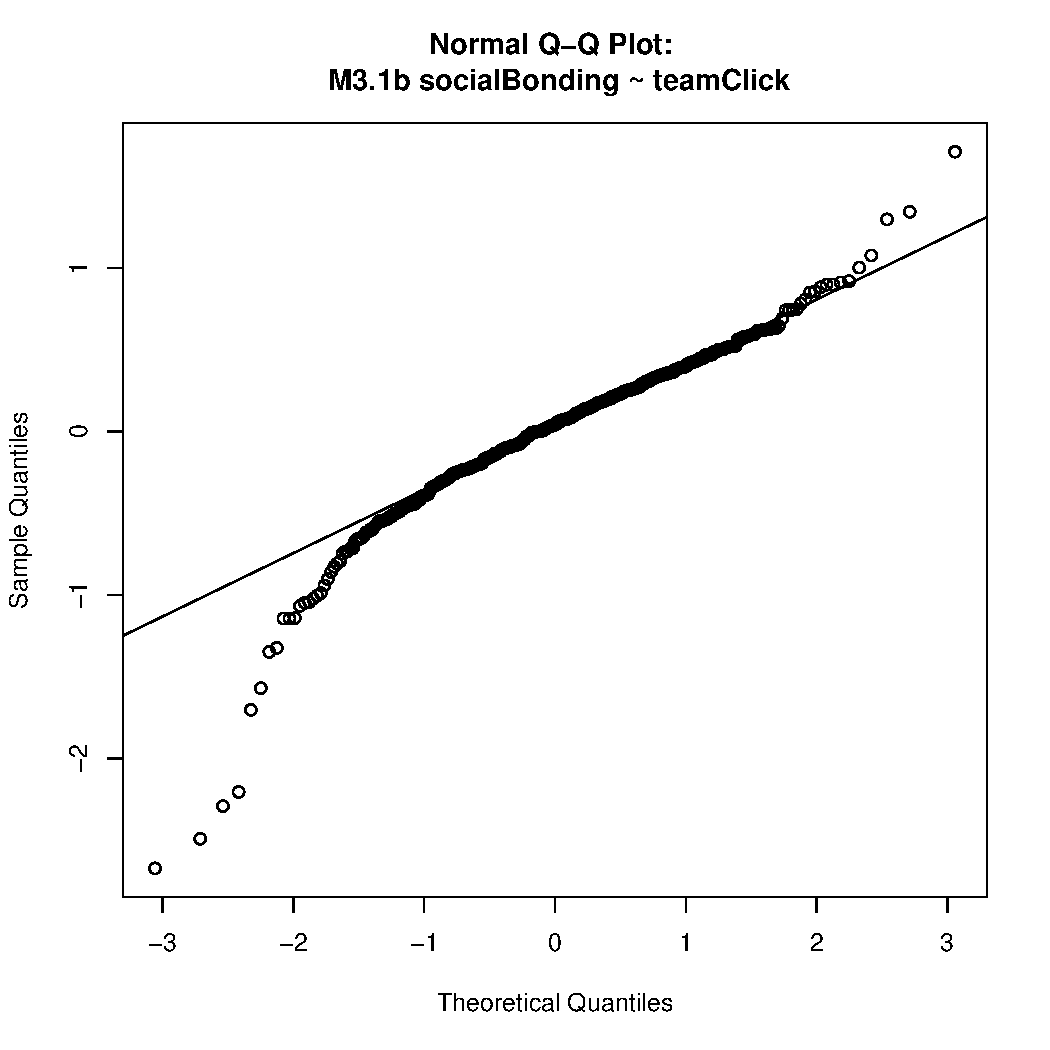
\includegraphics[scale =.4]{images/MLM31bQQNorm.pdf}
              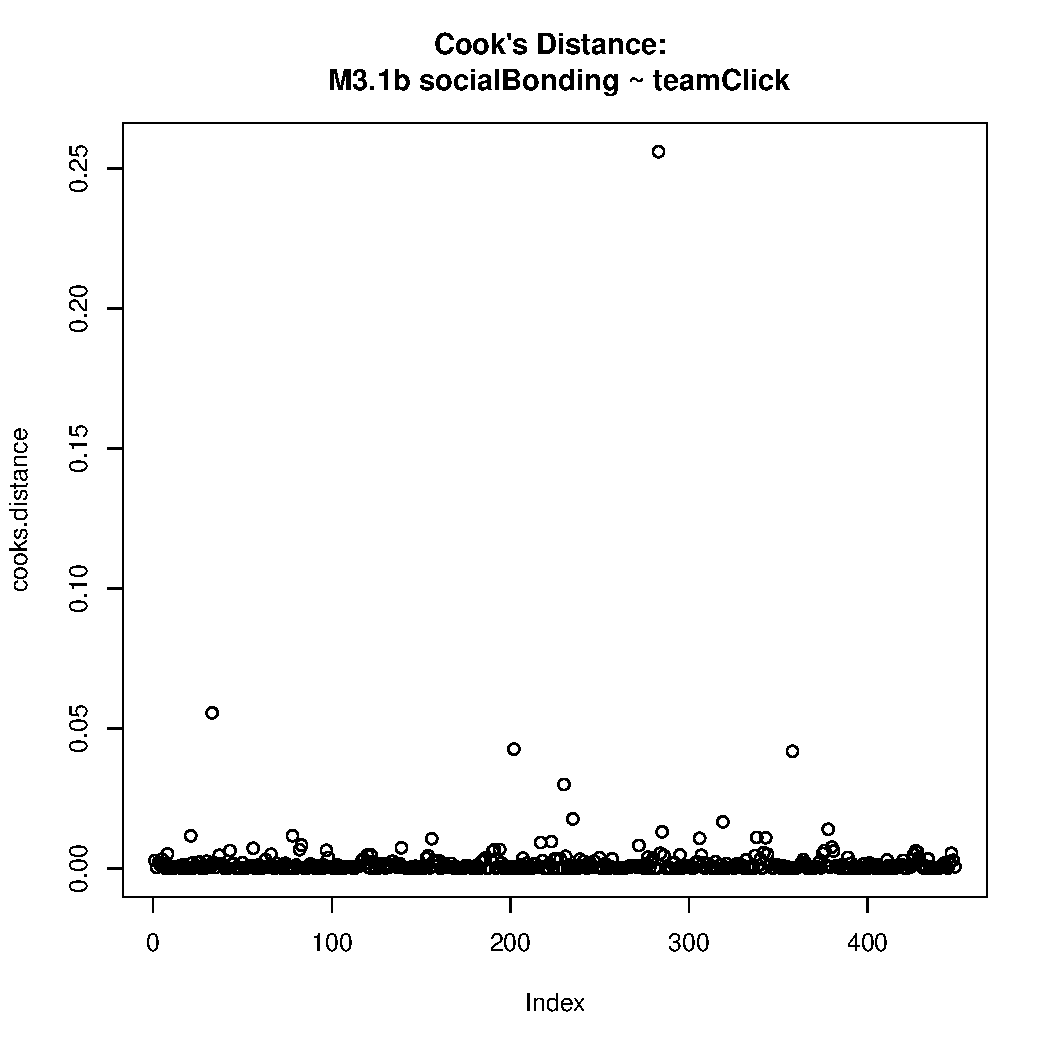
\includegraphics[scale =.4]{images/MLM31bCooksD.pdf}
              \caption{Model assumptions: Relationship between Team Click predicts Social Bonding (Overall Tournament)}
              \label{fig:MLM31bAssumptions}
            \end{figure}





       \subsubsection{Prediction 3: Team Performance Expectations predicts Team Click}


            \subsubsection{Post-Tournament}

                \myparagraph{Model comparisons}
                
% Table created by stargazer v.5.2 by Marek Hlavac, Harvard University. E-mail: hlavac at fas.harvard.edu
% Date and time: Mon, Jun 26, 2017 - 21:18:41
\begin{table}[!htbp] \centering 
  \caption{socialBonding = jointActionSuccess} 
  \label{tab:MLM3aJointActionSuccessBonding} 
\footnotesize 
\begin{tabular}{@{\extracolsep{5pt}}lccc} 
\\[-1.8ex]\hline 
\hline \\[-1.8ex] 
 & \multicolumn{3}{c}{\textit{Dependent variable:}} \\ 
\cline{2-4} 
\\[-1.8ex] & socialBonding & bondingPostFactorOut & bondingPostFactorLogReturned \\ 
 &  & outliers removed & log-transformed \\ 
\\[-1.8ex] & (1) & (2) & (3)\\ 
\hline \\[-1.8ex] 
 (constant) & $-$0.06 & $-$0.06 & 1.97$^{***}$ \\ 
  & (0.31) & (0.31) & (0.13) \\ 
  & & & \\ 
 jointActionSuccess & 0.45$^{**}$ & 0.45$^{**}$ & 0.20$^{***}$ \\ 
  & (0.14) & (0.14) & (0.06) \\ 
  & & & \\ 
 indPerformanceSuccess & 0.05 & 0.05 & $-$0.001 \\ 
  & (0.11) & (0.11) & (0.05) \\ 
  & & & \\ 
 objectiveCompetence & 0.07 & 0.07 & 0.04 \\ 
  & (0.10) & (0.10) & (0.04) \\ 
  & & & \\ 
 subjectiveCompetence & 0.19$^{*}$ & 0.19$^{*}$ & 0.09$^{*}$ \\ 
  & (0.08) & (0.08) & (0.03) \\ 
  & & & \\ 
 finalRank & $-$0.02 & $-$0.02 & $-$0.01 \\ 
  & (0.05) & (0.05) & (0.02) \\ 
  & & & \\ 
 minutesTotal & 0.002 & 0.002 & 0.001 \\ 
  & (0.004) & (0.004) & (0.002) \\ 
  & & & \\ 
 pointsTotal & $-$0.001 & $-$0.001 & $-$0.002 \\ 
  & (0.01) & (0.01) & (0.003) \\ 
  & & & \\ 
\hline \\[-1.8ex] 
Marginal R-squared & .27 & .18 & .28 \\ 
Conditional R-squared & .42 & .34 & .43 \\ 
Observations & 97 & 97 & 97 \\ 
Log Likelihood & $-$113.05 & $-$113.05 & $-$29.49 \\ 
Akaike Inf. Crit. & 250.10 & 250.10 & 82.98 \\ 
Bayesian Inf. Crit. & 281.00 & 281.00 & 113.87 \\ 
\hline 
\hline \\[-1.8ex] 
\textit{Note:}  & \multicolumn{3}{r}{$^{*}$p$<$0.05; $^{**}$p$<$0.01; $^{***}$p$<$0.001} \\ 
\end{tabular} 
\end{table} 



            \begin{figure}[htbp]
              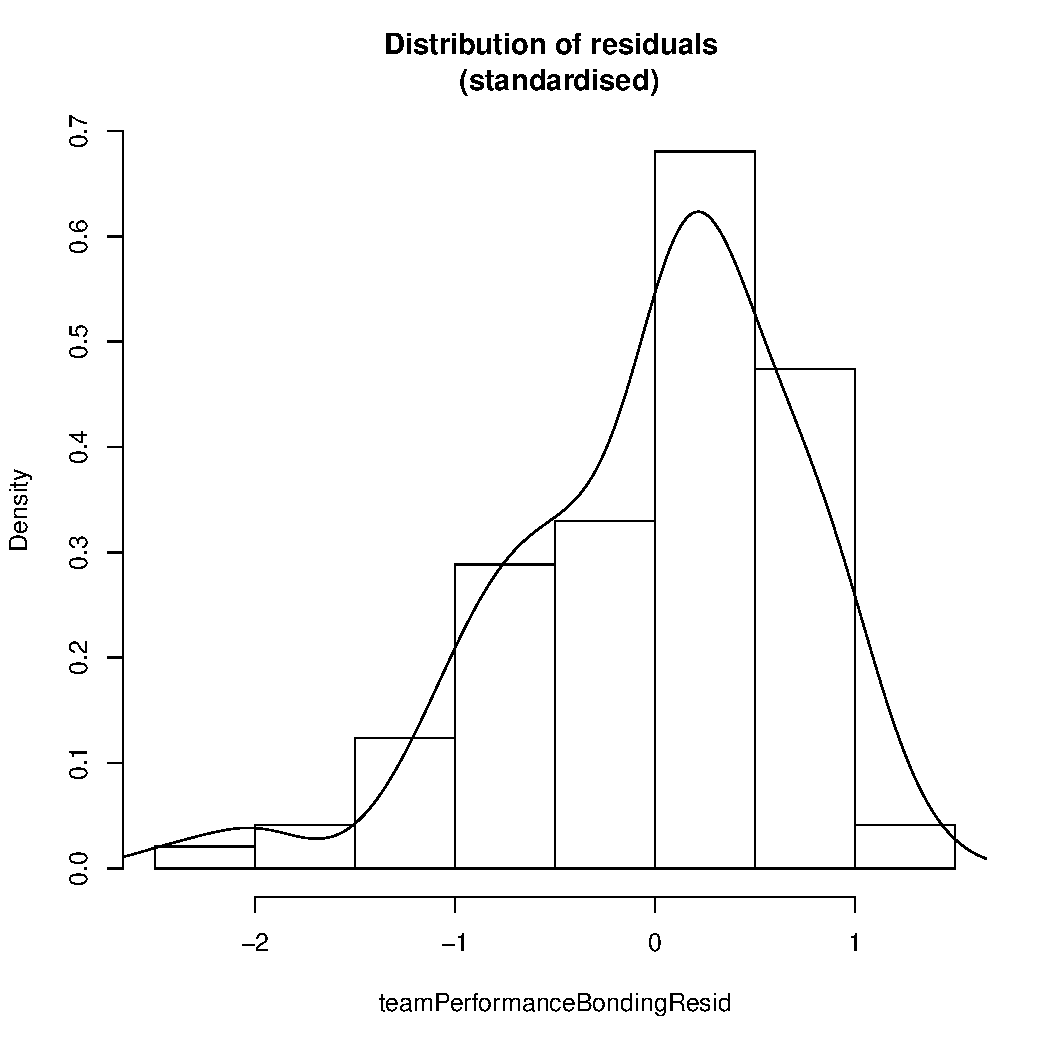
\includegraphics[scale =.4]{images/MLM3aHist.pdf}
              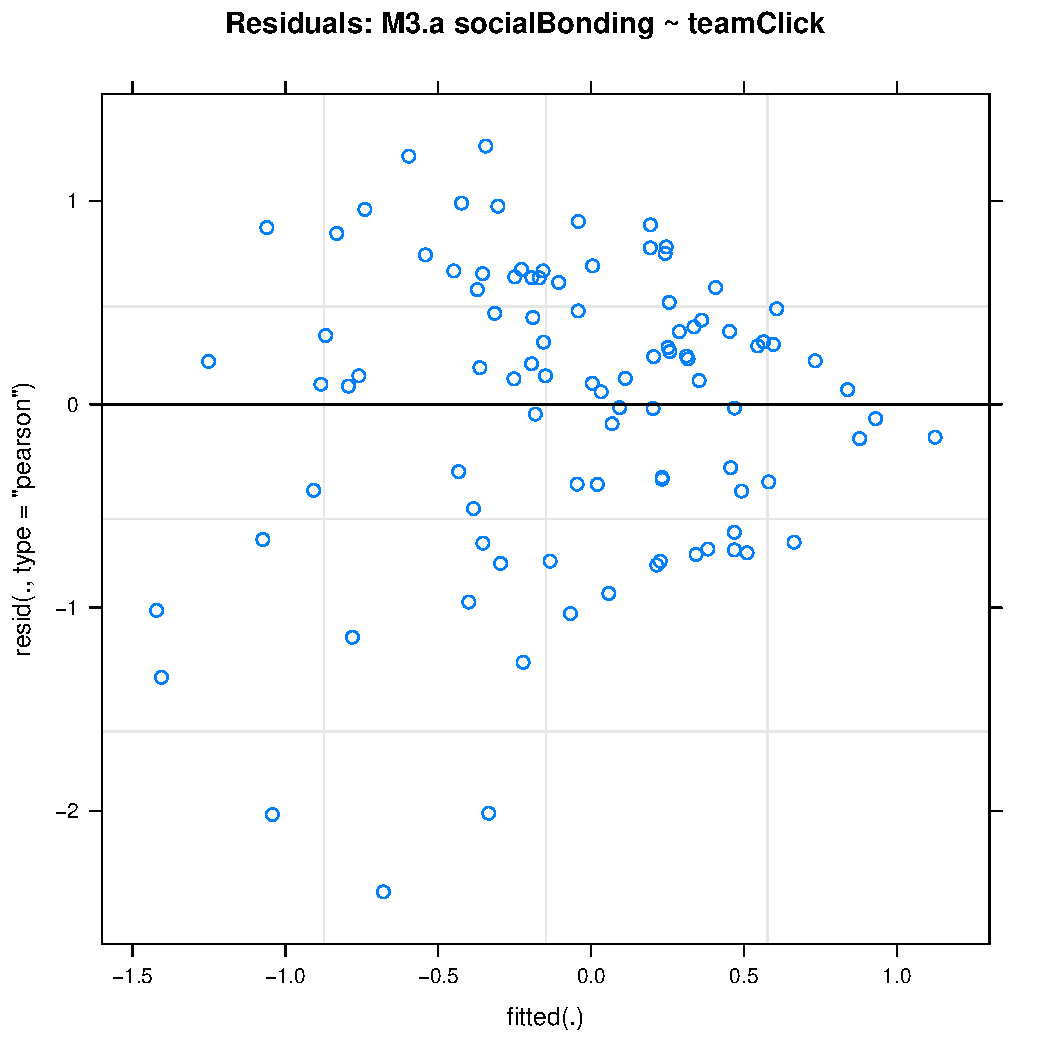
\includegraphics[scale =.4]{images/MLM3aScatter.pdf}
              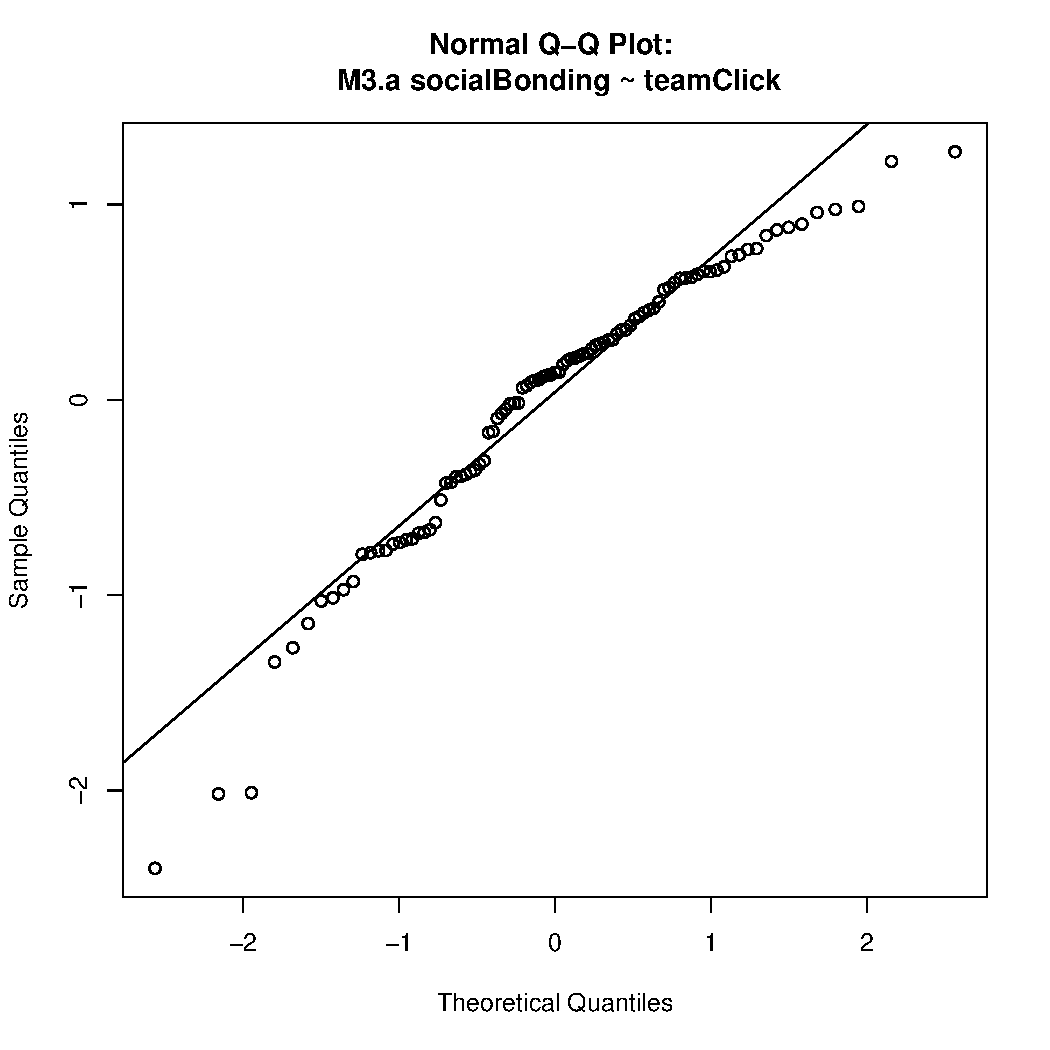
\includegraphics[scale =.4]{images/MLM3aQQNorm.pdf}
              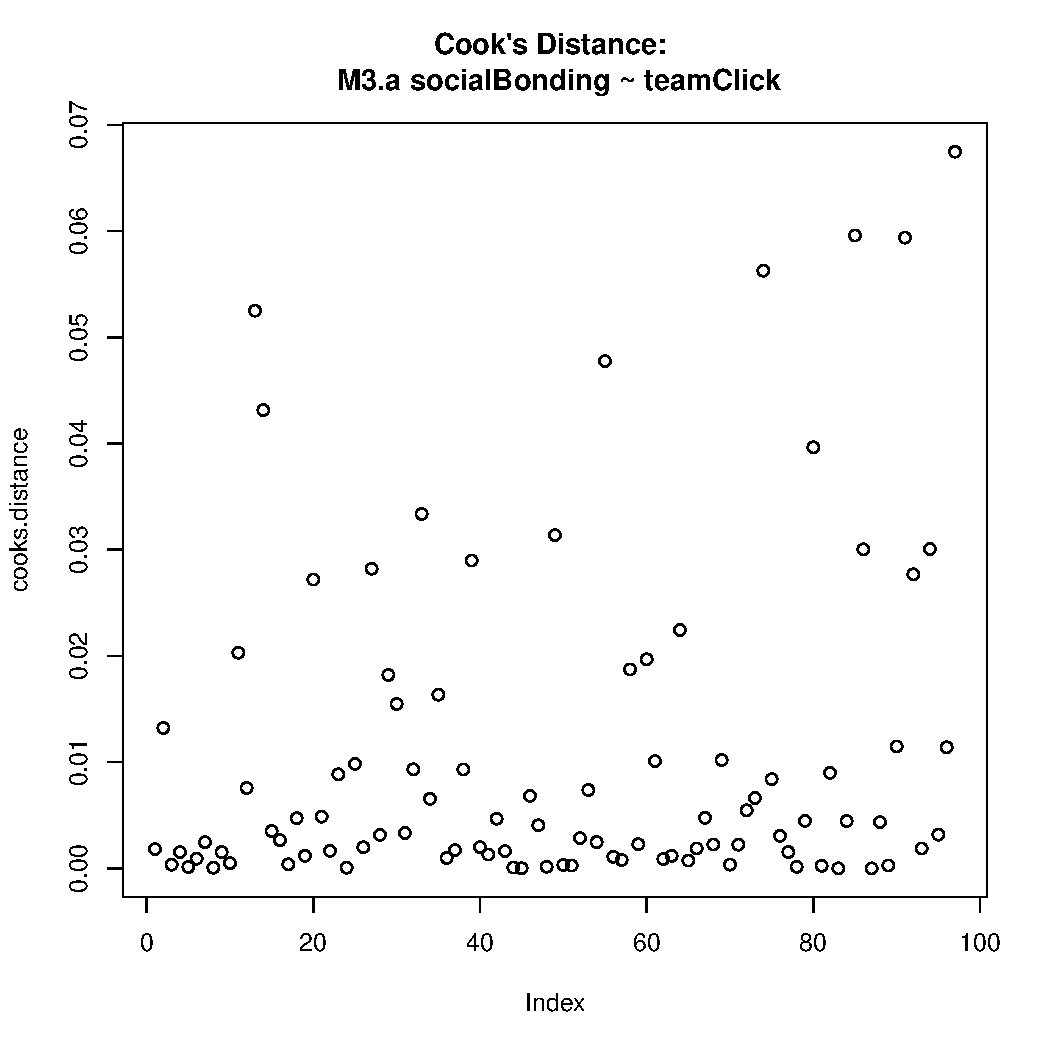
\includegraphics[scale =.4]{images/MLM3aCooksD.pdf}
              \caption{Model assumptions: M3a Team Performance Components predict Social Bonding}
              \label{fig:MLM3aAssumptions}
            \end{figure}


            \begin{figure}[htbp]
              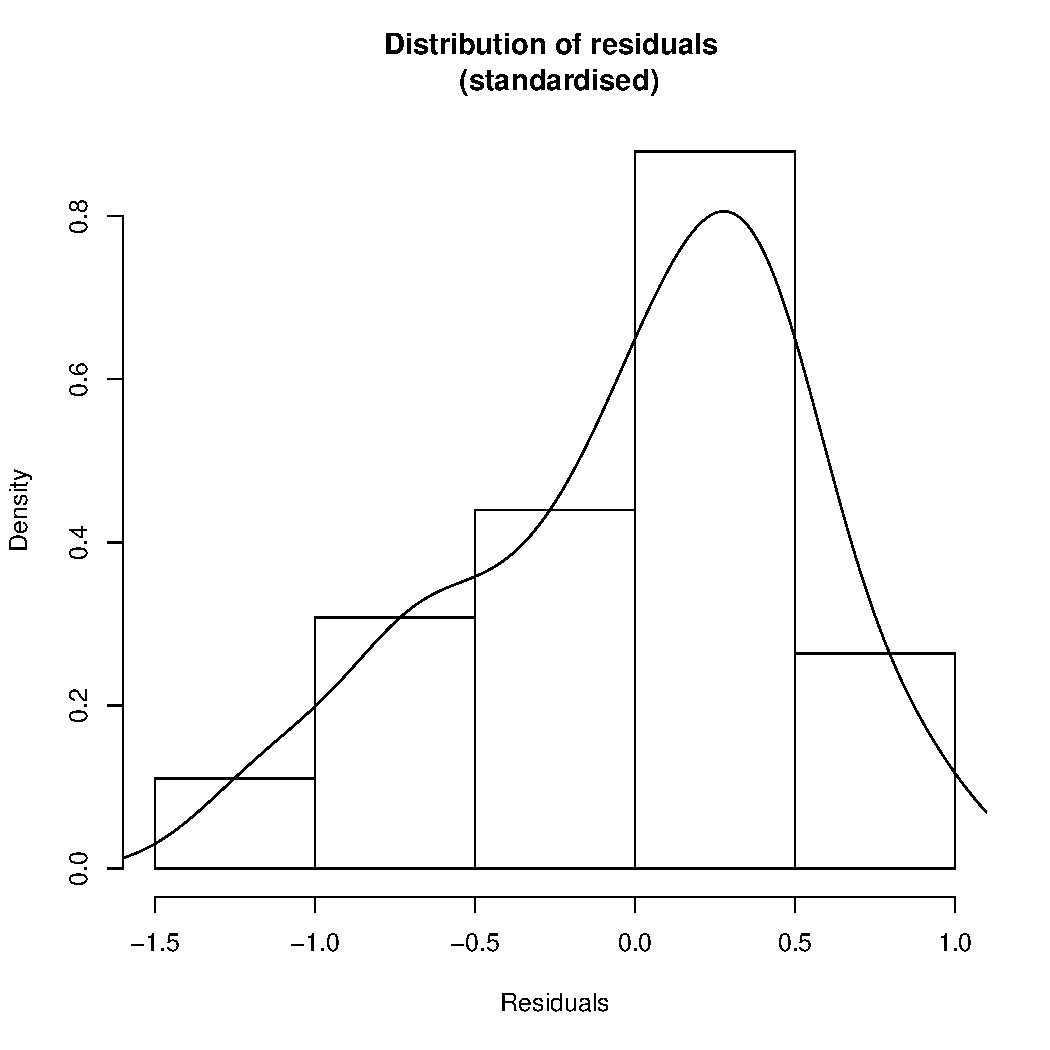
\includegraphics[scale =.4]{images/MLM3aOutHist.pdf}
              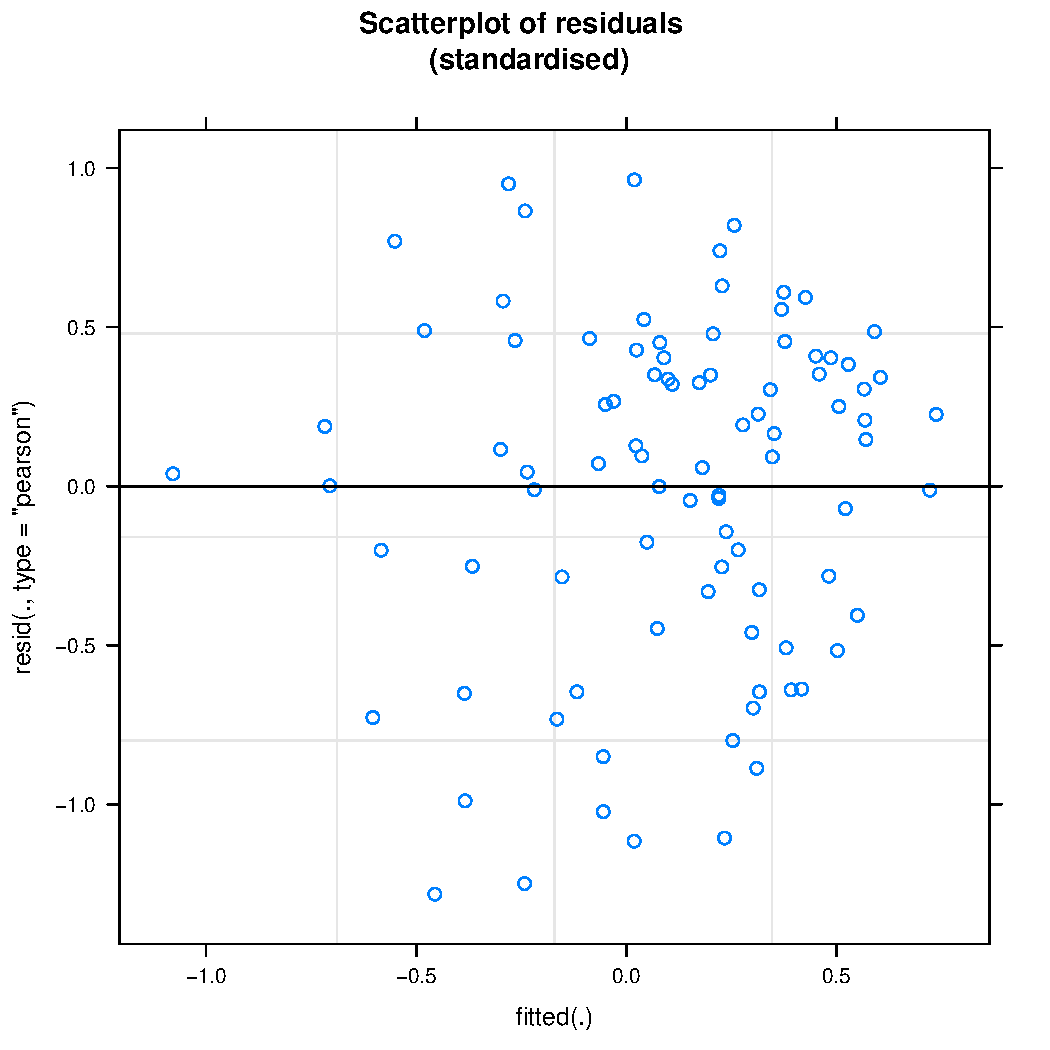
\includegraphics[scale =.4]{images/MLM3aOutScatter.pdf}
              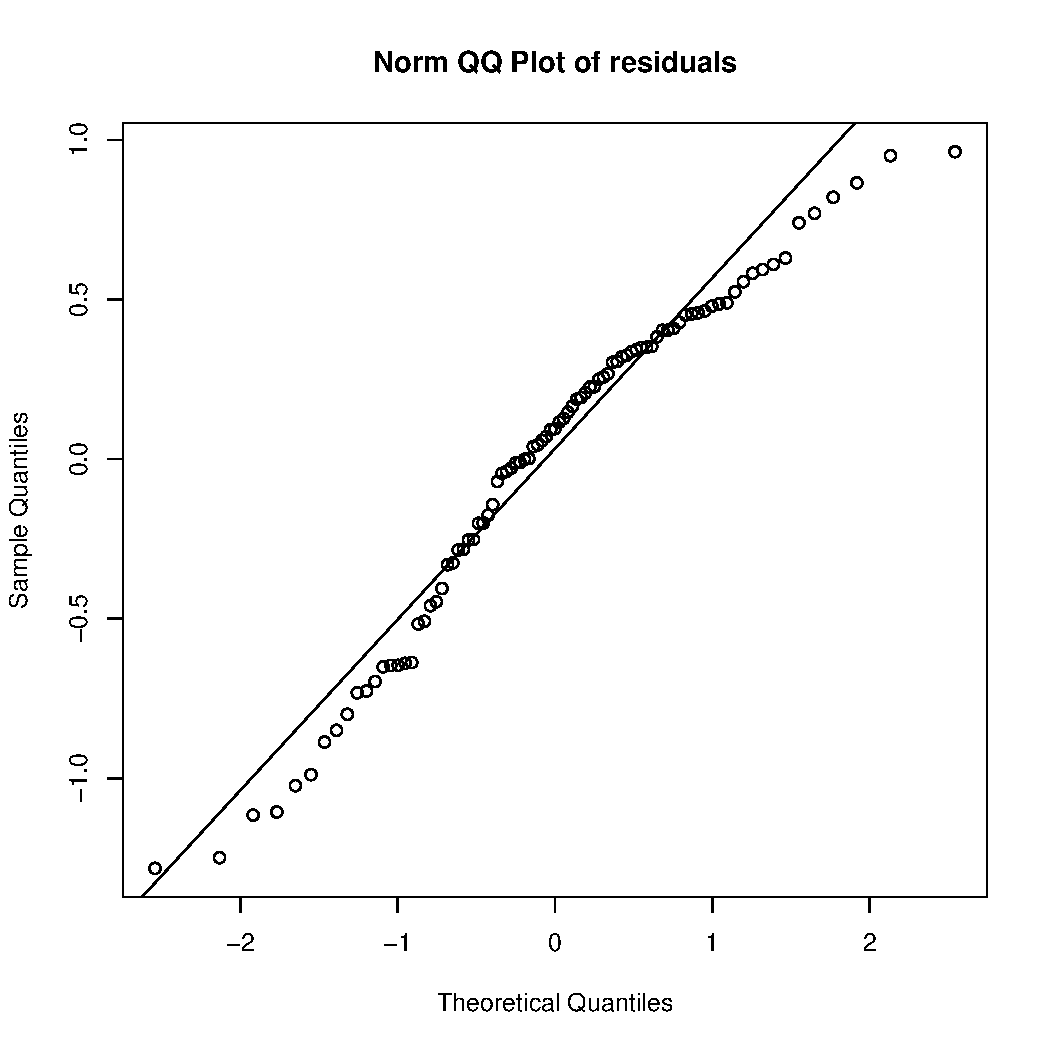
\includegraphics[scale =.4]{images/MLM3aOutQQNorm.pdf}
              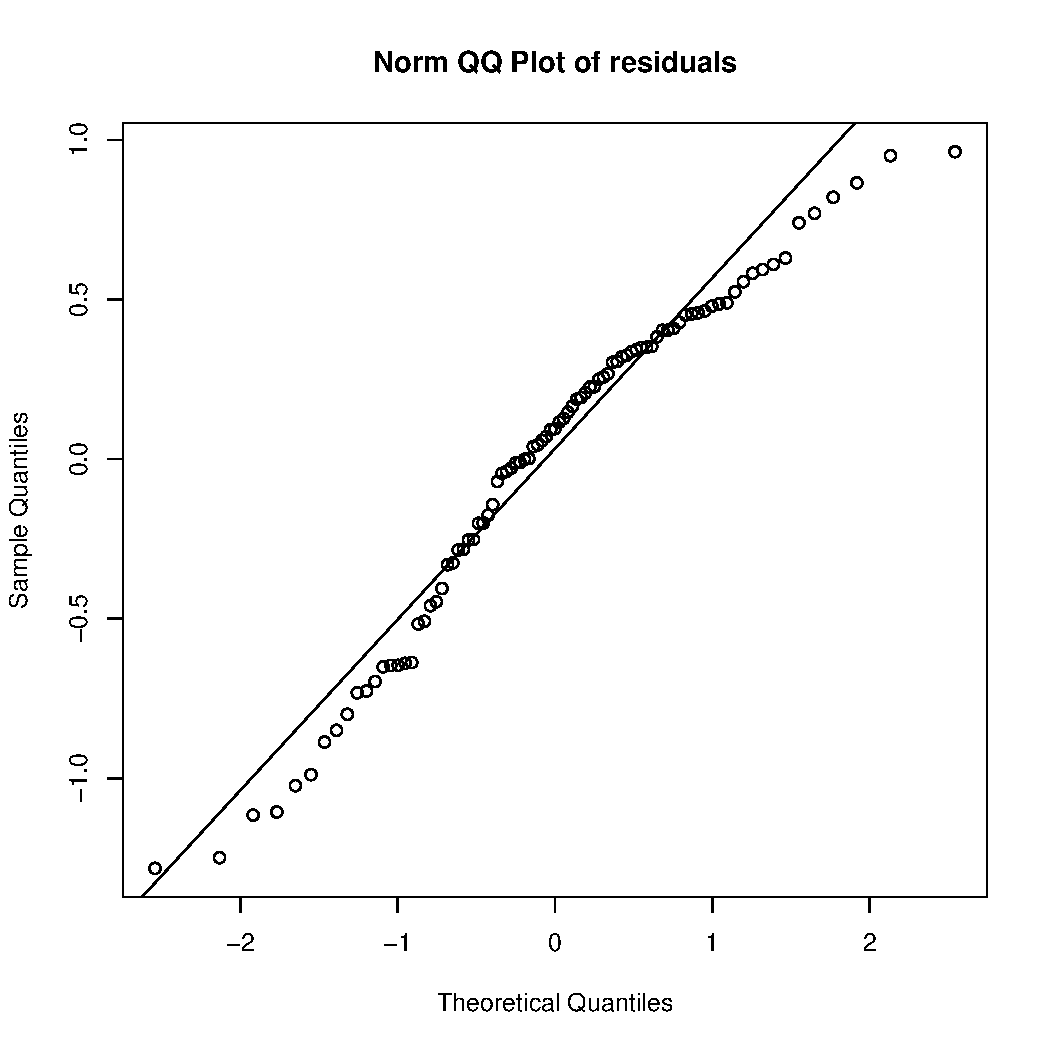
\includegraphics[scale =.4]{images/MLM3aOutCooksD.pdf}
              \caption{Model assumptions: Team Performance Components predicts Social Bonding (outliers removed)}
             \label{fig:MLM3aOutAssumptions}
            \end{figure}


            \begin{figure}[htbp]
              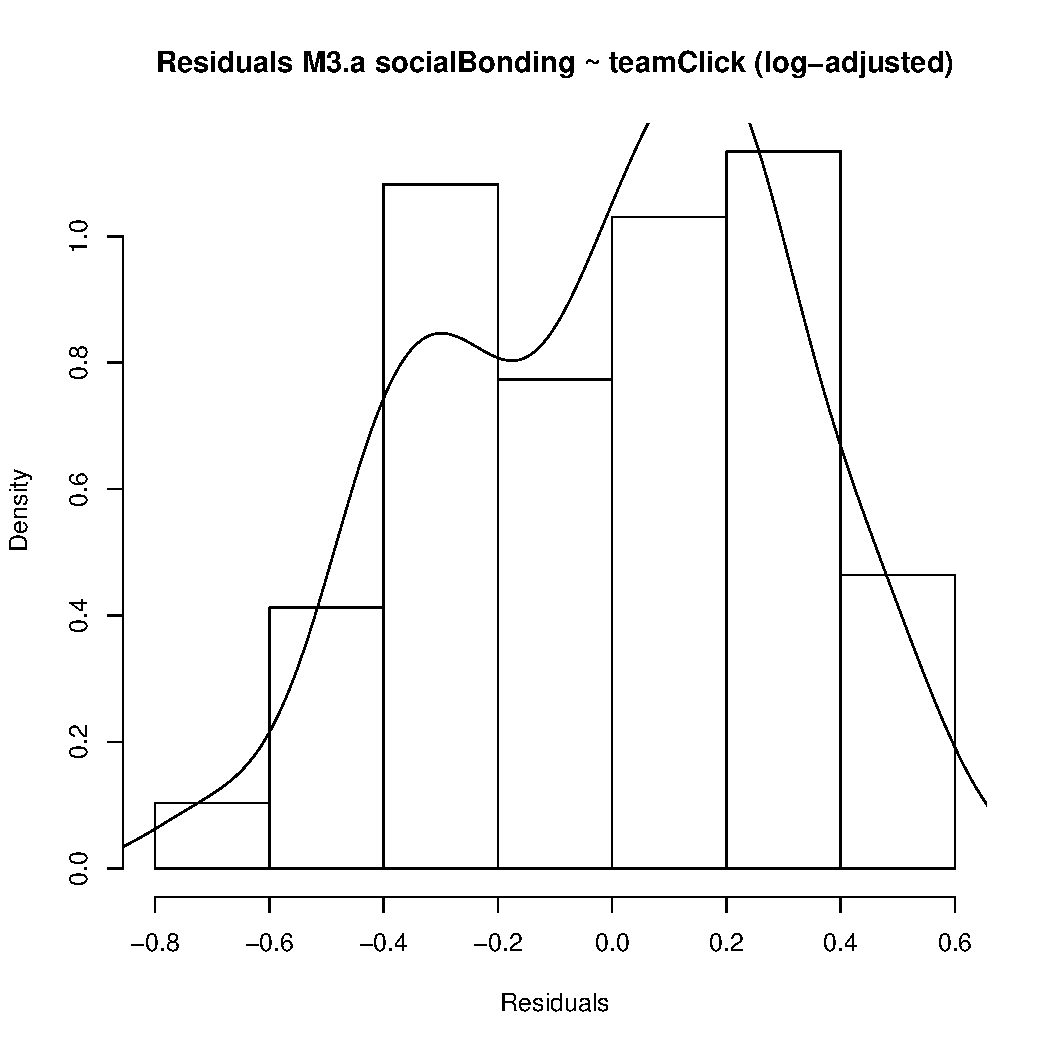
\includegraphics[scale =.4]{images/MLM3aLogHist.pdf}
              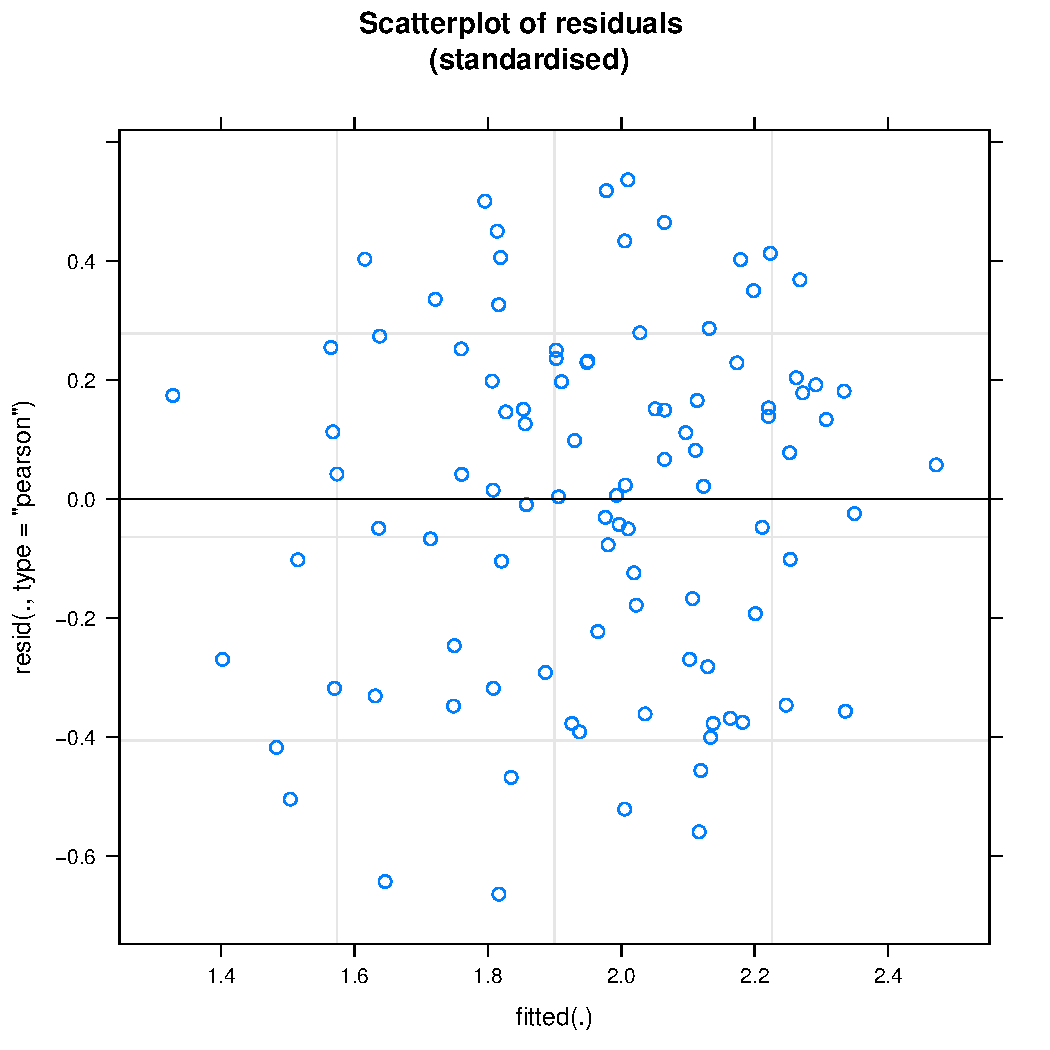
\includegraphics[scale =.4]{images/MLM3aLogScatter.pdf}
              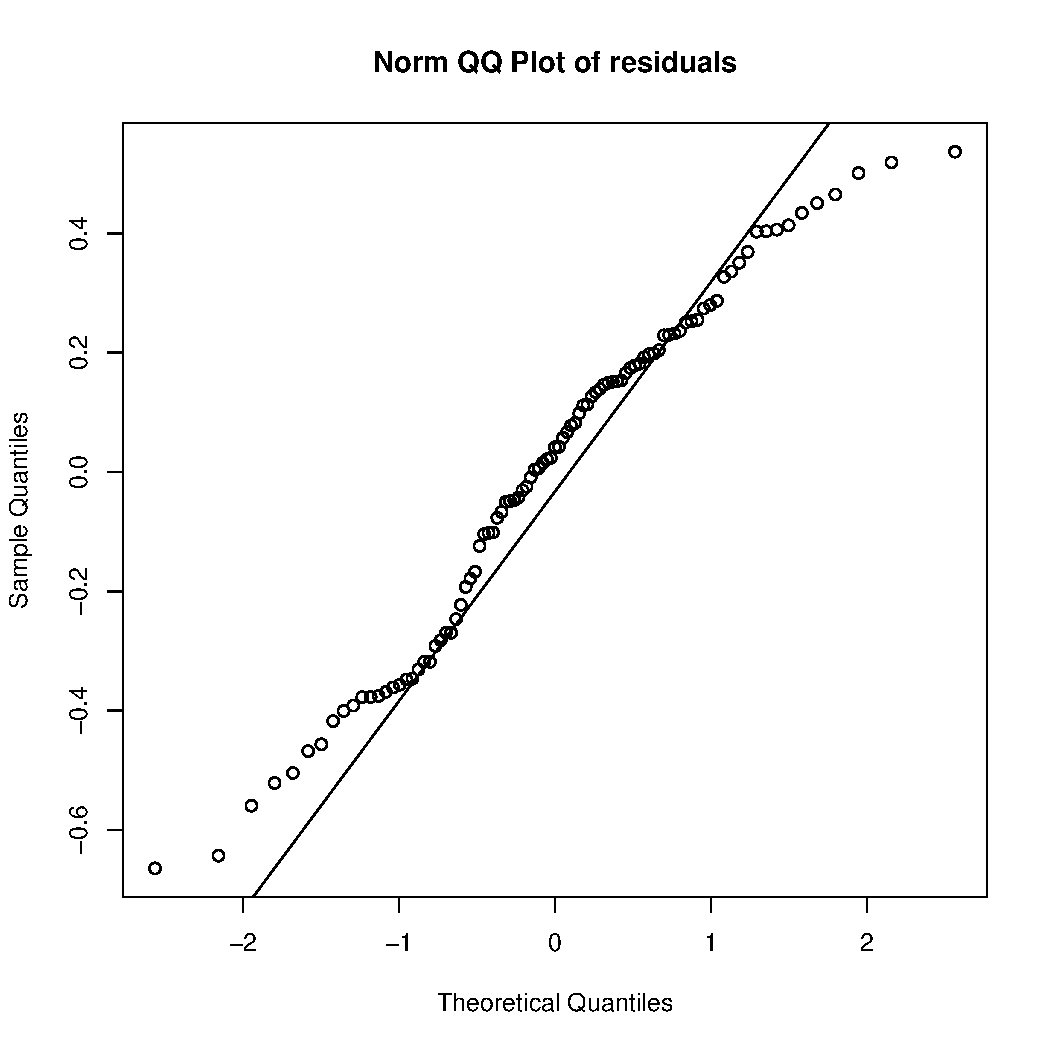
\includegraphics[scale =.4]{images/MLM3aLogQQNorm.pdf}
              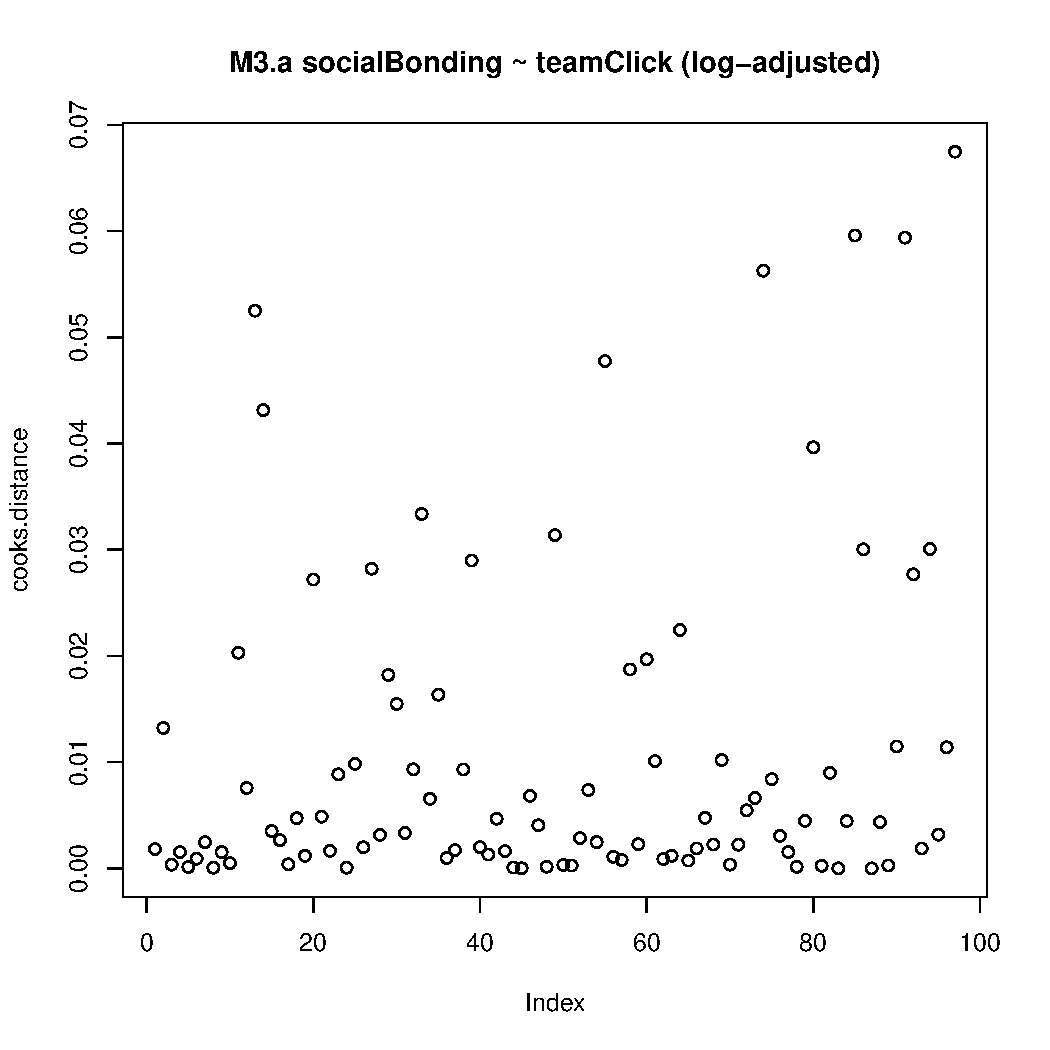
\includegraphics[scale =.4]{images/MLM3aLogCooksD.pdf}
              \caption{Model assumptions: Team Performance Components predicts Social Bonding (log-transformed)}
              \label{fig:MLM3aLogAssumptions}
            \end{figure}







            \subsubsection{Pre- to Post Tournament\label{app8:MLM23a}}


            
\begin{table}
\begin{center}
\begin{tabular}{l c c c }
\toprule
 & Controls & Outliers removed & Log-adjusted \\
\midrule
(constant)                                               & $\mathbf{0.34}^{***}$ & $\mathbf{0.35}^{***}$ & $0.22$                \\
                                                         & $(0.09)$              & $(0.09)$              & $(0.46)$              \\
Team Performance Components Change                       &                       & $\mathbf{0.24}^{***}$ & $\mathbf{0.36}^{***}$ \\
                                                         &                       & $(0.07)$              & $(0.09)$              \\
Ind Performance Components Change                        &                       &                       & $-0.21$               \\
                                                         &                       &                       & $(0.11)$              \\
Objective Competence                                     &                       &                       & $0.17$                \\
                                                         &                       &                       & $(0.11)$              \\
Subjective Competence                                    &                       &                       & $0.03$                \\
                                                         &                       &                       & $(0.09)$              \\
Final Rank                                               &                       &                       & $-0.02$               \\
                                                         &                       &                       & $(0.05)$              \\
Minutes Total                                            &                       &                       & $0.01$                \\
                                                         &                       &                       & $(0.00)$              \\
Points Total                                             &                       &                       & $0.00$                \\
                                                         &                       &                       & $(0.01)$              \\
Fatigue                                                  &                       &                       & $-0.18$               \\
                                                         &                       &                       & $(0.10)$              \\
Extraverted                                              &                       &                       & $-0.03$               \\
                                                         &                       &                       & $(0.06)$              \\
\midrule
AIC                                                      & 265.55                & 260.75                & 240.96                \\
BIC                                                      & 273.34                & 276.32                & 275.96                \\
Log Likelihood                                           & -129.78               & -124.37               & -106.48               \\
Num. obs.                                                & 99                    & 99                    & 90                    \\
Num. groups: team                                        & 14                    & 14                    & 13        \\           
\bottomrule
\multicolumn{4}{l}{\scriptsize{Coefficients with $p < 0.05$ in \textbf{bold}. Effect sizes for log-transformed model: Marginal $R^2 = .18$, Conditional $R^2 = .18$}}
\end{tabular}
\caption{Prediction 3: Team Performance Components Change predict Social Bonding Change in the Pre- to Post-Tournament survey data (n = 97).}
\label{tab:MLM23aJointActionSuccessBonding}
\end{center}
\end{table}



            \subsubsection{Overall Tournament}

            \begin{figure}[htbp]
              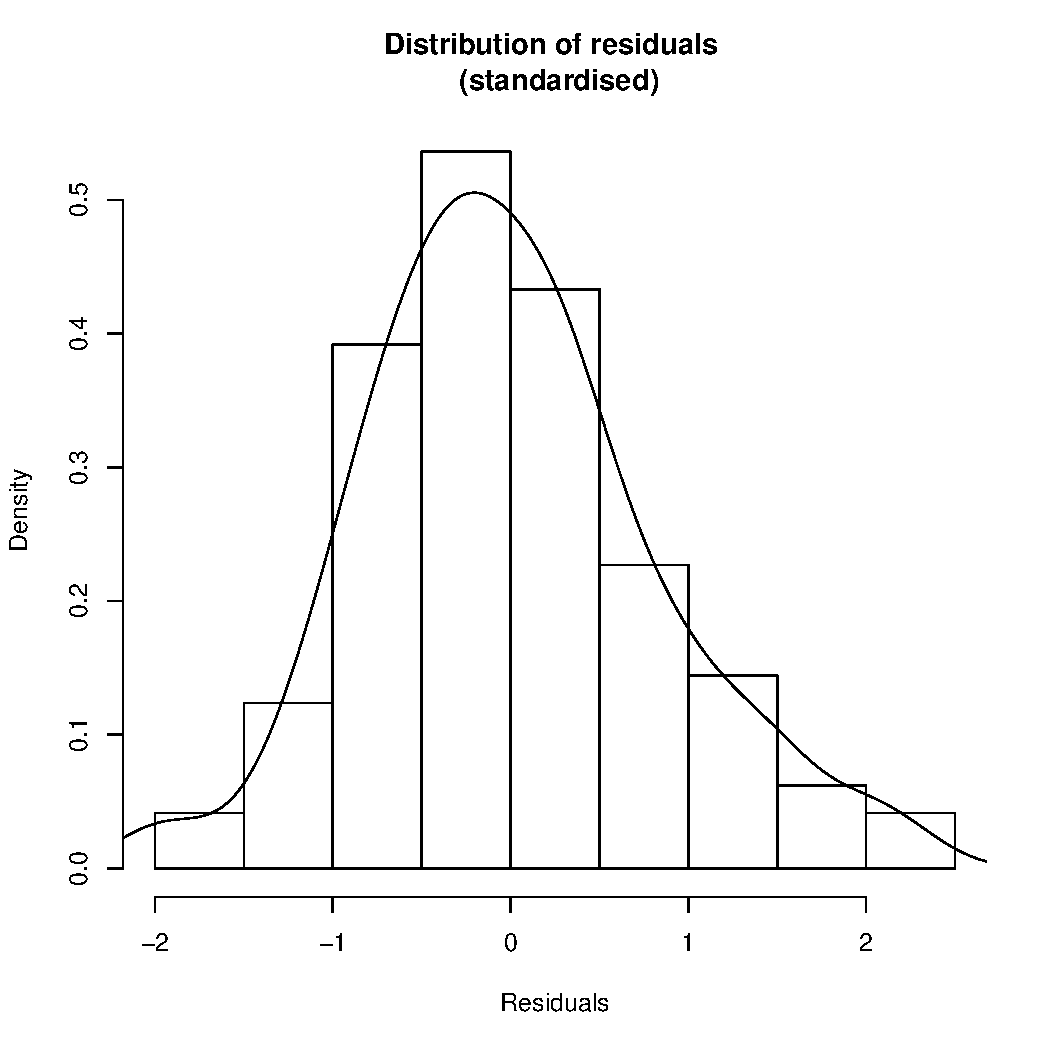
\includegraphics[scale =.4]{images/MLM23aHist.pdf}
              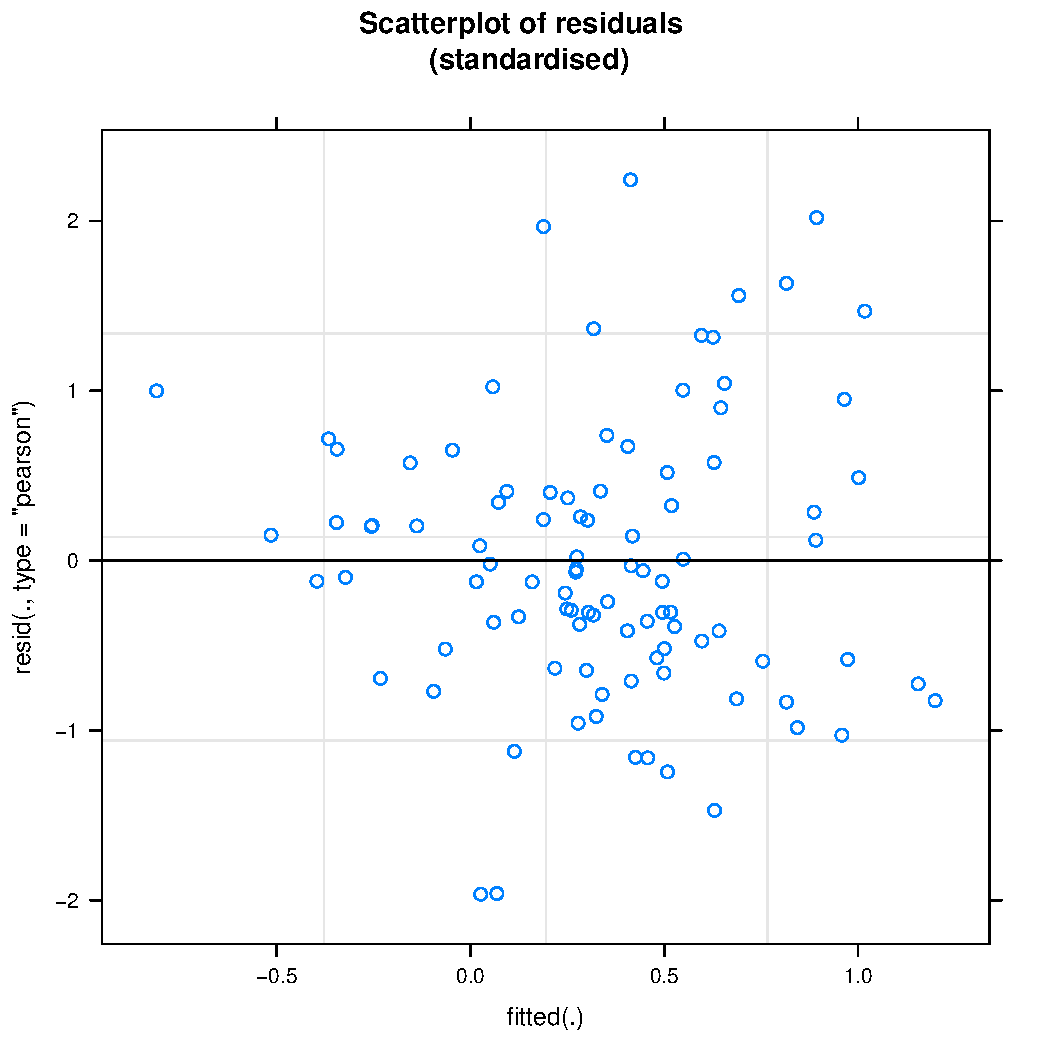
\includegraphics[scale =.4]{images/MLM23aScatter.pdf}
              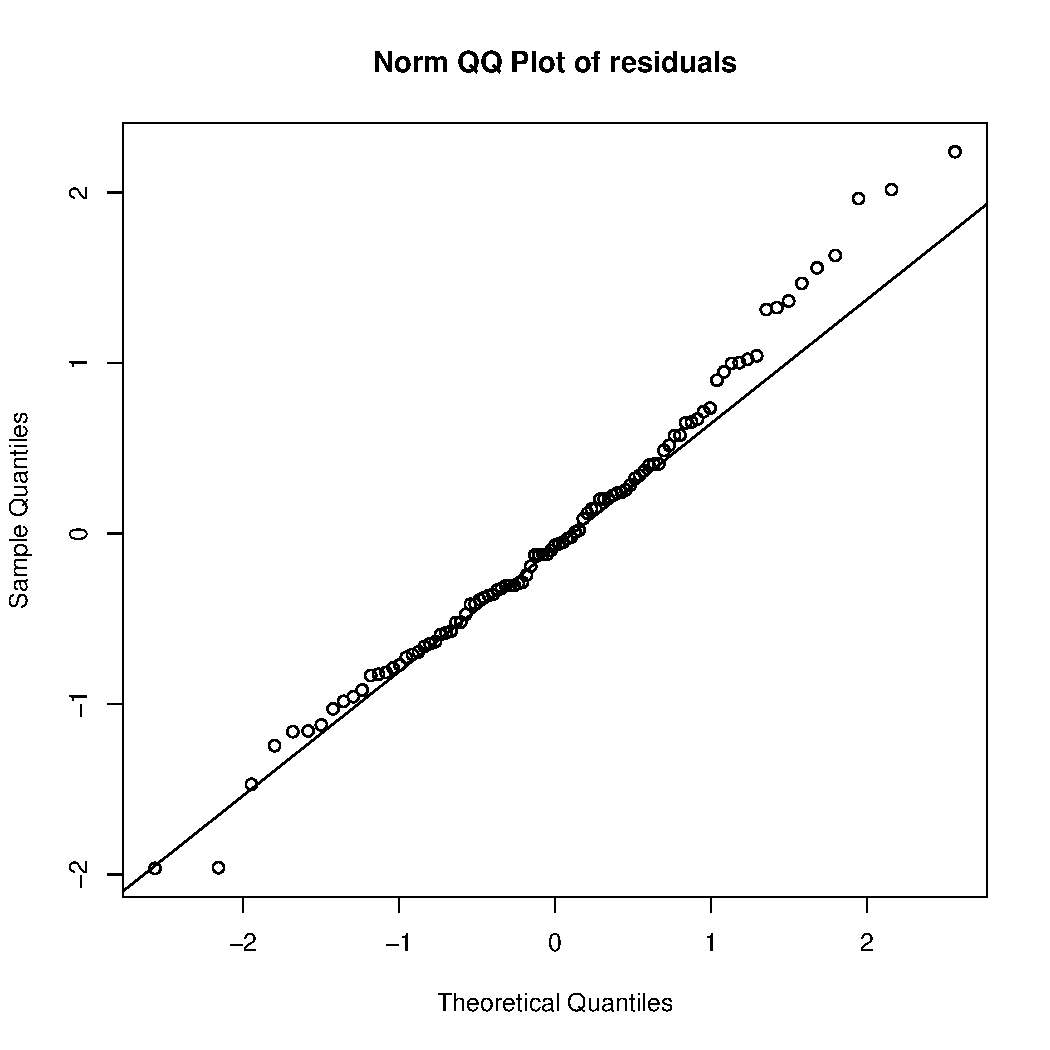
\includegraphics[scale =.4]{images/MLM23aQQNorm.pdf}
              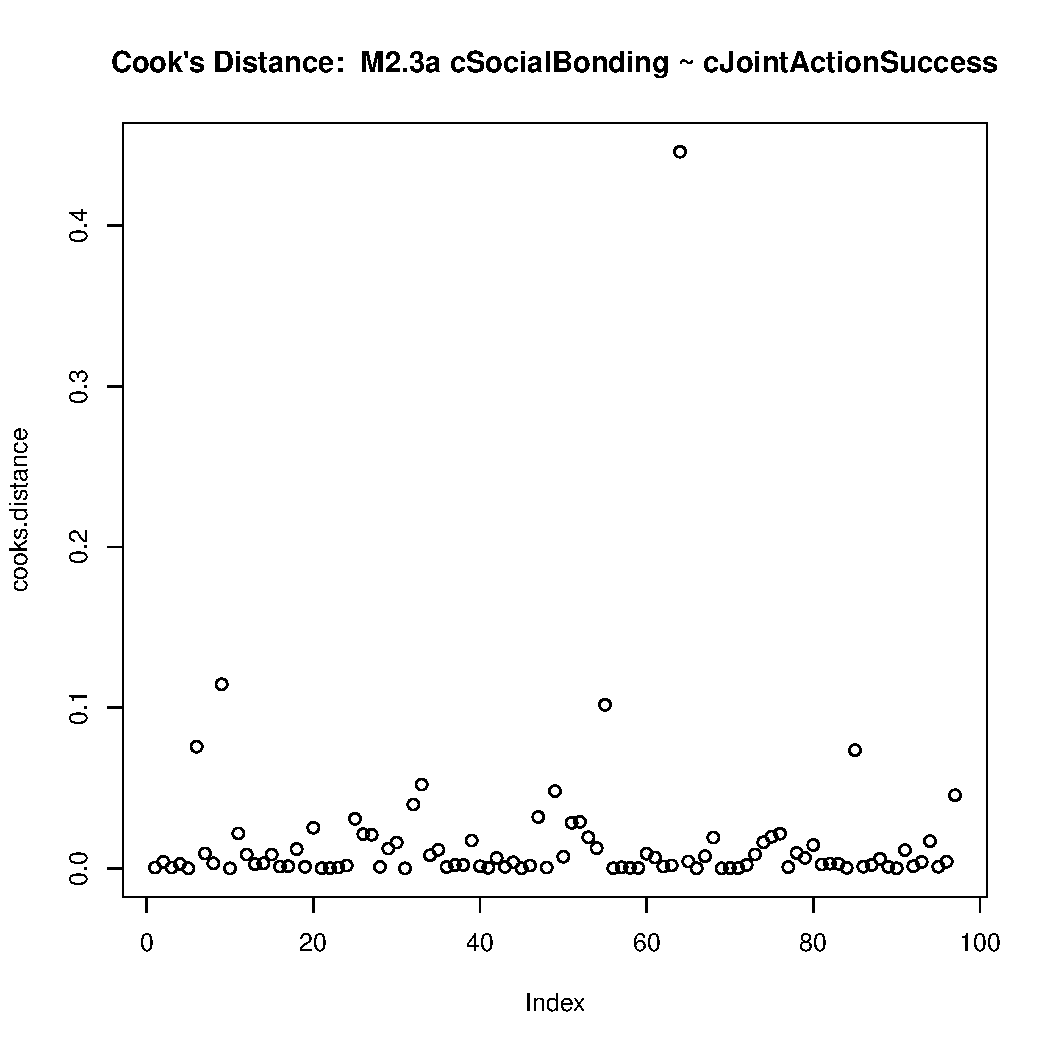
\includegraphics[scale =.4]{images/MLM23aCooksD.pdf}
              \caption{Model assumptions: Team Performance Components Change predicts Social Bonding Change}
              \label{fig:MLM23aAssumptions}
            \end{figure}






%%  \subsection{4: Team Click mediates the relationship between Team Performance Components and Social Bonding}

%\subsubsection{Post-Tournament}

  % \begin{figure}[htbp]
  %   \centering
  %   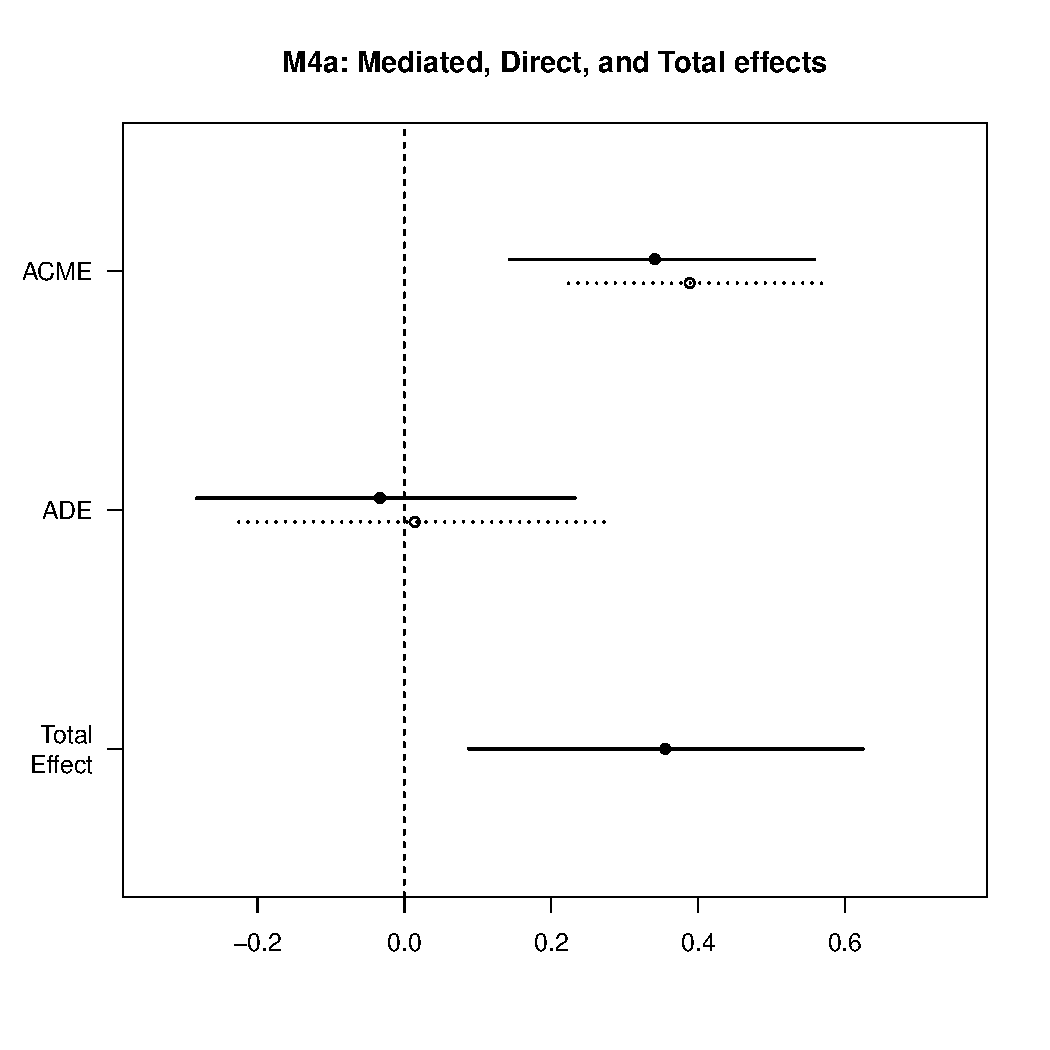
\includegraphics[scale = .5]{images/MLM4aMediationEffects.pdf}
  %   \caption{M4a Mediation Analysis}
  %   \label{fig:MLM4aMediationAnalysis}
  % \end{figure}

%\myparagraph{Model robustness checks}

%\subsubsection{Pre- to Post-Tournament}


%  \begin{figure}[htbp]
%  \centering
%  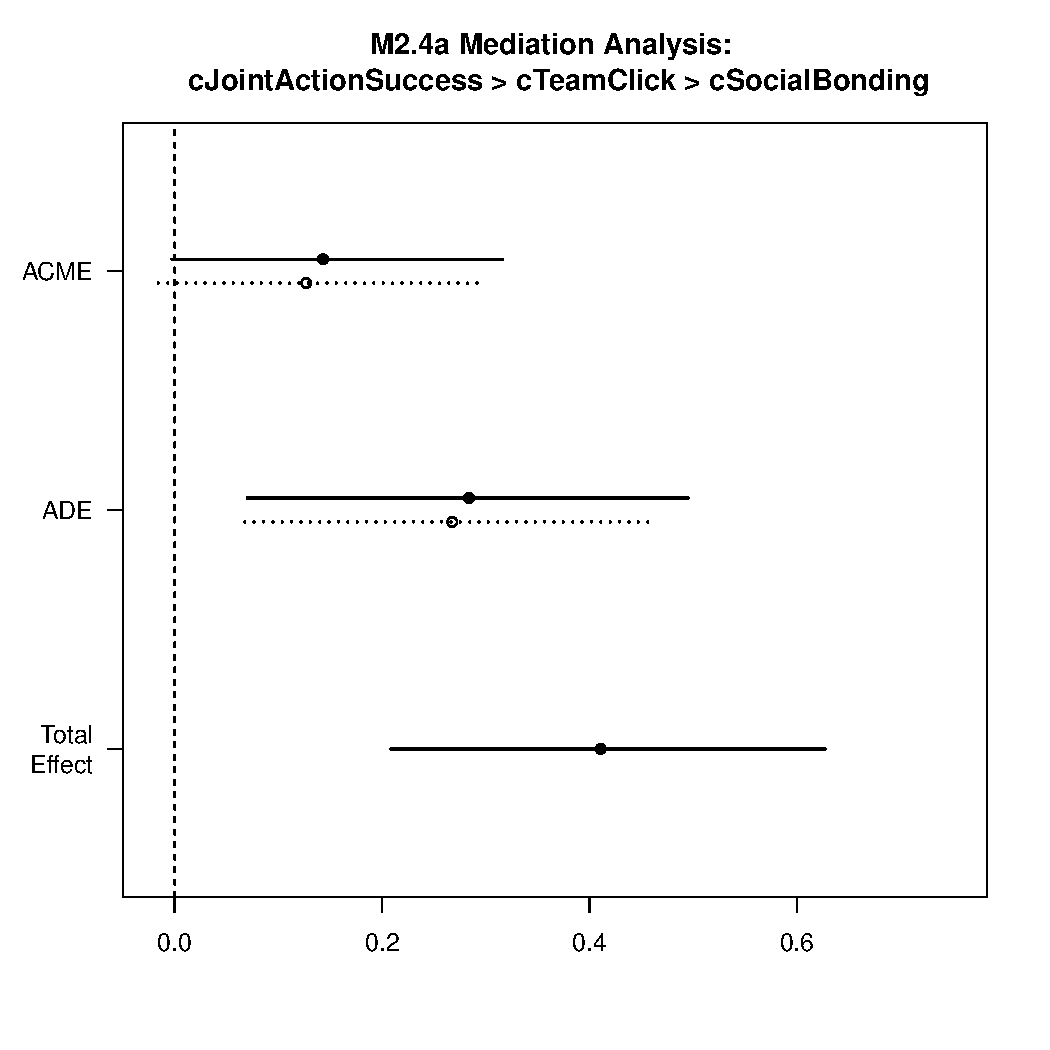
\includegraphics[scale=.5]{images/MLM24aMediationAnalysis.pdf}
%  \caption{M24a Mediation Analysis}
%  \label{fig:MLM24aMediationAnalysis}
%\end{figure}
%\myparagraph{Model robustness checks}

%  \subsubsection{Overall Tournament}

%%       \begin{figure}[htbp]
%       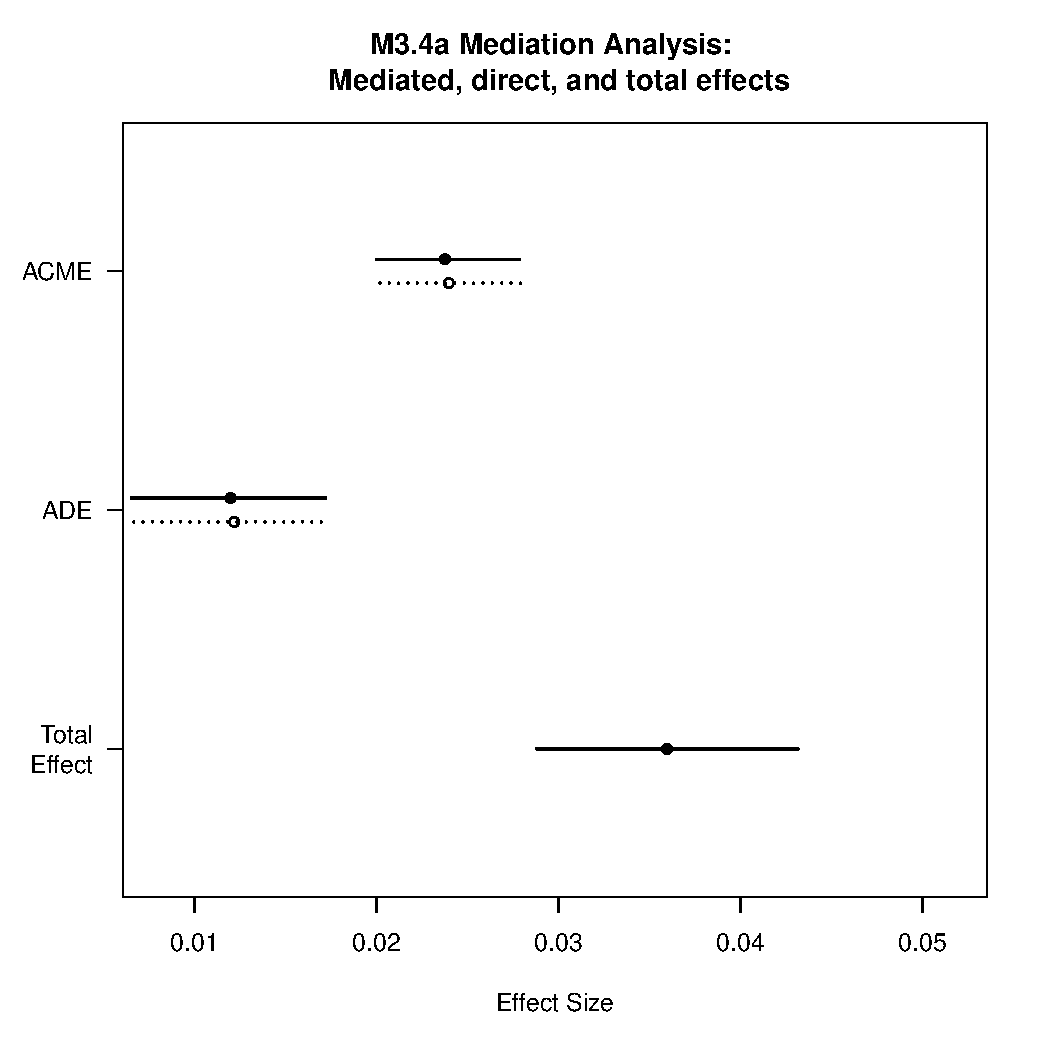
\includegraphics[scale=.5]{images/MLM34aMediationAnalysis.pdf}
  %     \caption{M3.4a Mediation Analysis}
  %     \label{fig:MLM34aMediationAnalysis}
  %   \end{figure}

%\myparagraph{Model robustness checks}







       \subsubsection{Prediction 5.1: Team Performance Expectations predicts Team Click}


       \subsubsection{Post-Tournament}

      %   \begin{align*}
      %     Team Click =  Team Performance Expectations \\
      %               + Individual Performance Expectations \\
      %               + Objective Competence + Subjective Competence \\
      %               + Tournament performance measures \\
      %   \end{align*}


            
\begin{table}
\begin{center}
\begin{tabular}{l c c c }
\toprule
 & Intercept & Main effect & Controls \\
\midrule
(constant)                                 & $-0.04$  & $-0.00$               & $\mathbf{-0.79}^{*}$  \\
                                           & $(0.15)$ & $(0.09)$              & $(0.40)$              \\
Team Performance Vs Expectations           &          & $\mathbf{0.50}^{***}$ & $\mathbf{0.51}^{***}$ \\
                                           &          & $(0.11)$              & $(0.12)$              \\
Ind Performance Vs Expectations            &          &                       & $0.02$                \\
                                           &          &                       & $(0.08)$              \\
Objective Competence                       &          &                       & $0.02$                \\
                                           &          &                       & $(0.08)$              \\
Subjective Competence                      &          &                       & $0.12$                \\
                                           &          &                       & $(0.07)$              \\
Final Rank                                 &          &                       & $\mathbf{0.09}^{*}$   \\
                                           &          &                       & $(0.05)$              \\
Minutes Total                              &          &                       & $-0.00$               \\
                                           &          &                       & $(0.00)$              \\
Points Total                               &          &                       & $0.00$                \\
                                           &          &                       & $(0.01)$              \\
Fatigue                                    &          &                       & $\mathbf{0.18}^{*}$   \\
                                           &          &                       & $(0.09)$              \\
Extraverted                                &          &                       & $0.06$                \\
                                           &          &                       & $(0.05)$              \\
\midrule
AIC                                        & 299.06   & 268.43                & 228.63                \\
BIC                                        & 307.37   & 285.06                & 264.68                \\
Log Likelihood                             & -146.53  & -128.22               & -100.32               \\
Num. obs.                                  & 118      & 118                   & 97                    \\
Num. groups: team                          & 15       & 15                    & 14                    \\
\bottomrule
\multicolumn{4}{l}{\scriptsize{Coefficients with $p < 0.05$ in \textbf{bold}. Marginal $R^2 = .40$, Conditional $R^2 = .56$}}
\end{tabular}
\caption{Prediction 5: Team Performance Vs Expectations predicts Team Click in the Post-Tournament survey data (n = 97).}
\label{tab:MLM1bteamExpectationsClick}
\end{center}
\end{table}



       \begin{figure}[htbp]
         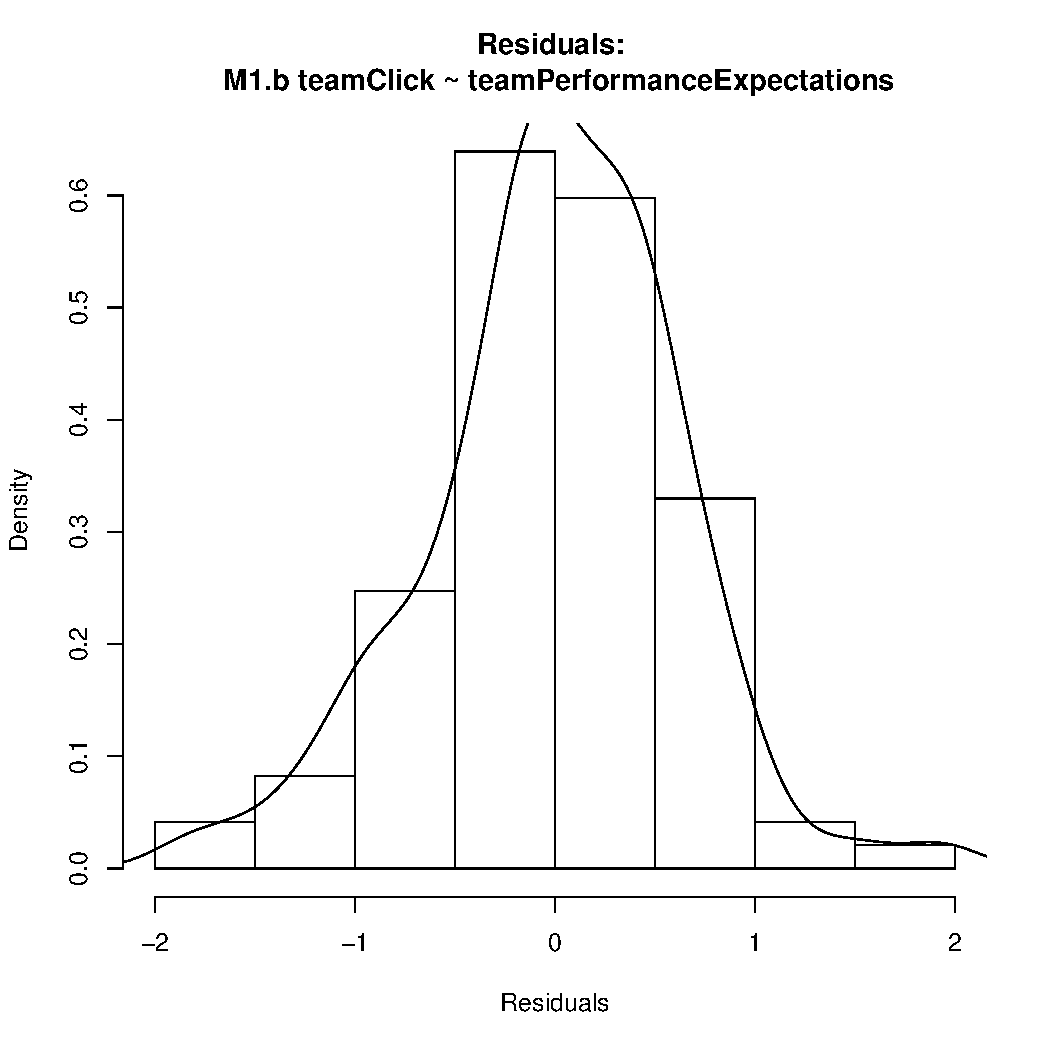
\includegraphics[scale =.4]{images/MLM1bHist.pdf}
         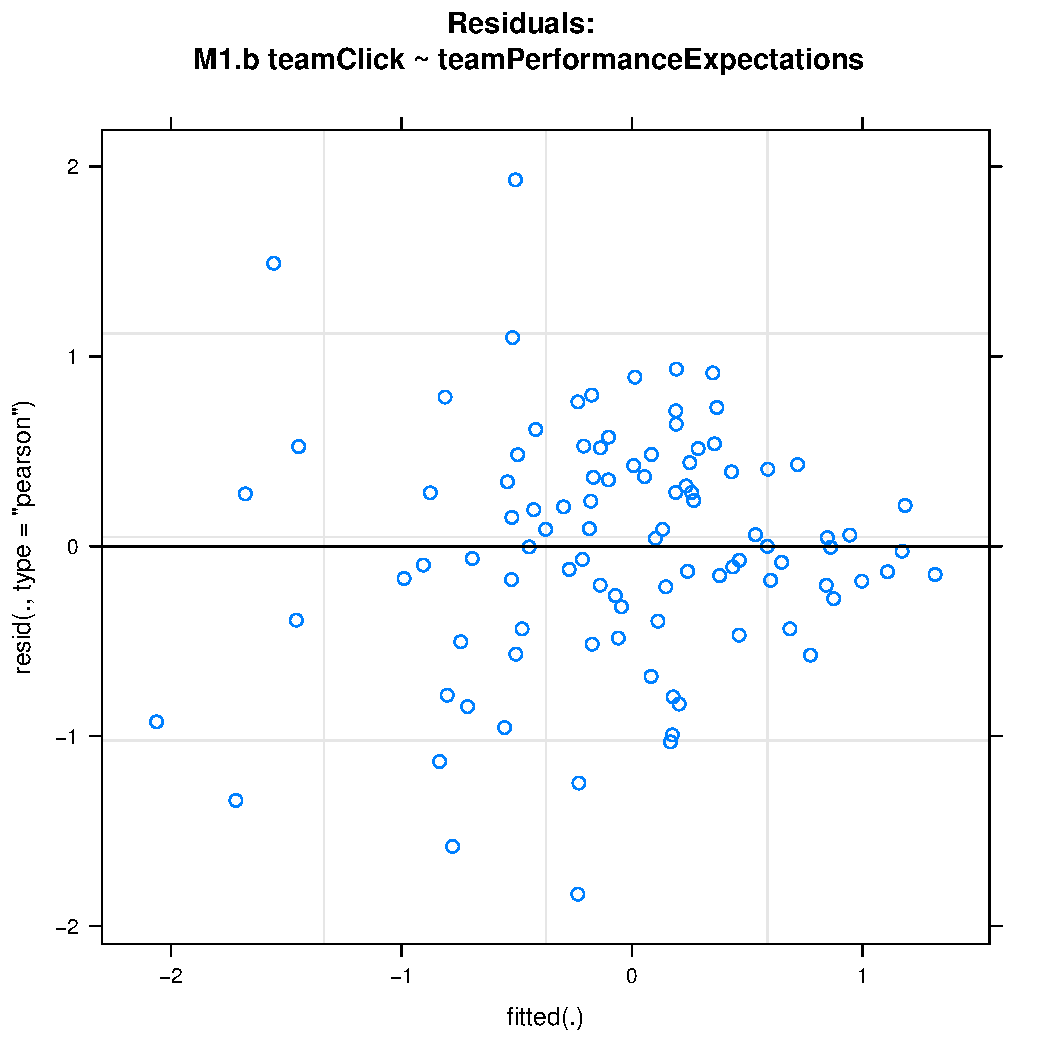
\includegraphics[scale =.4]{images/MLM1bScatter.pdf}
         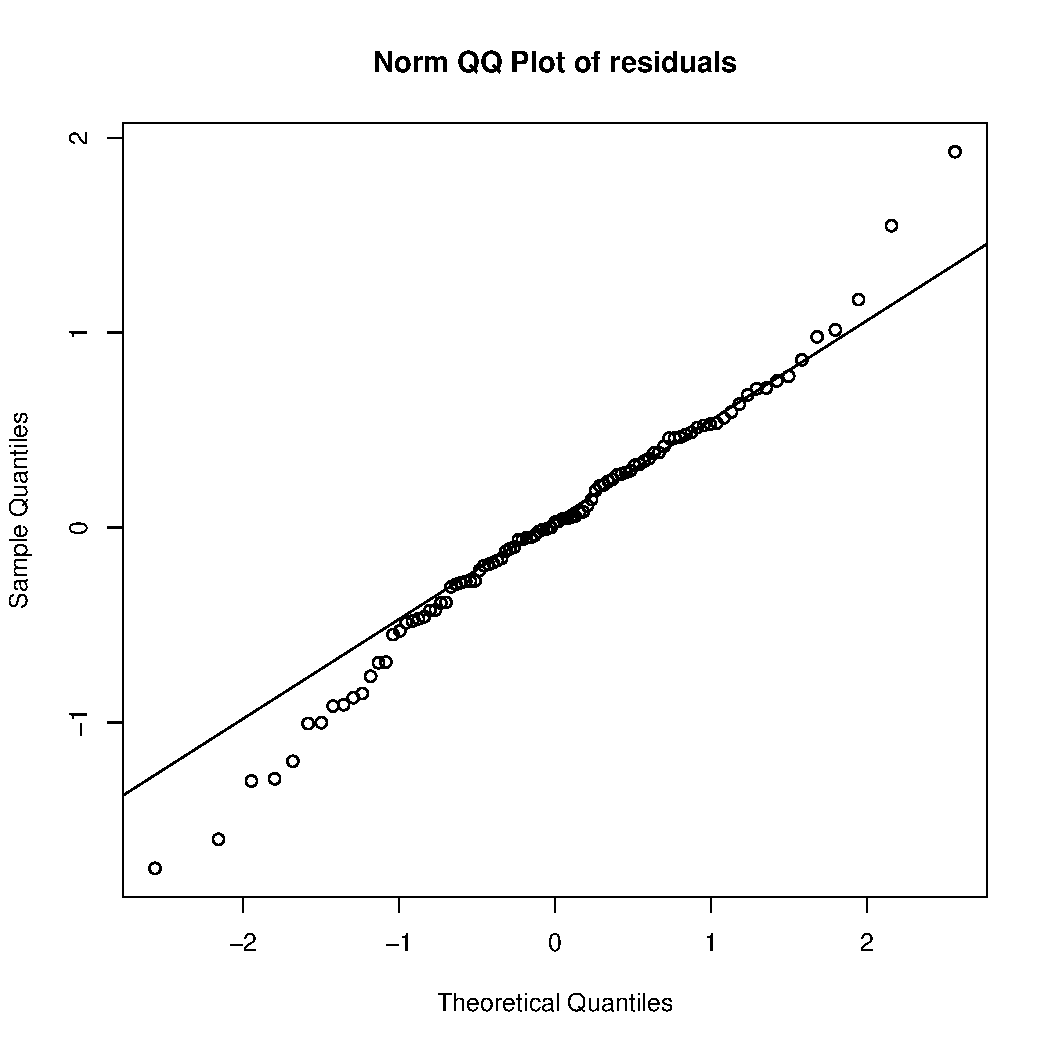
\includegraphics[scale =.4]{images/MLM1bQQNorm.pdf}
         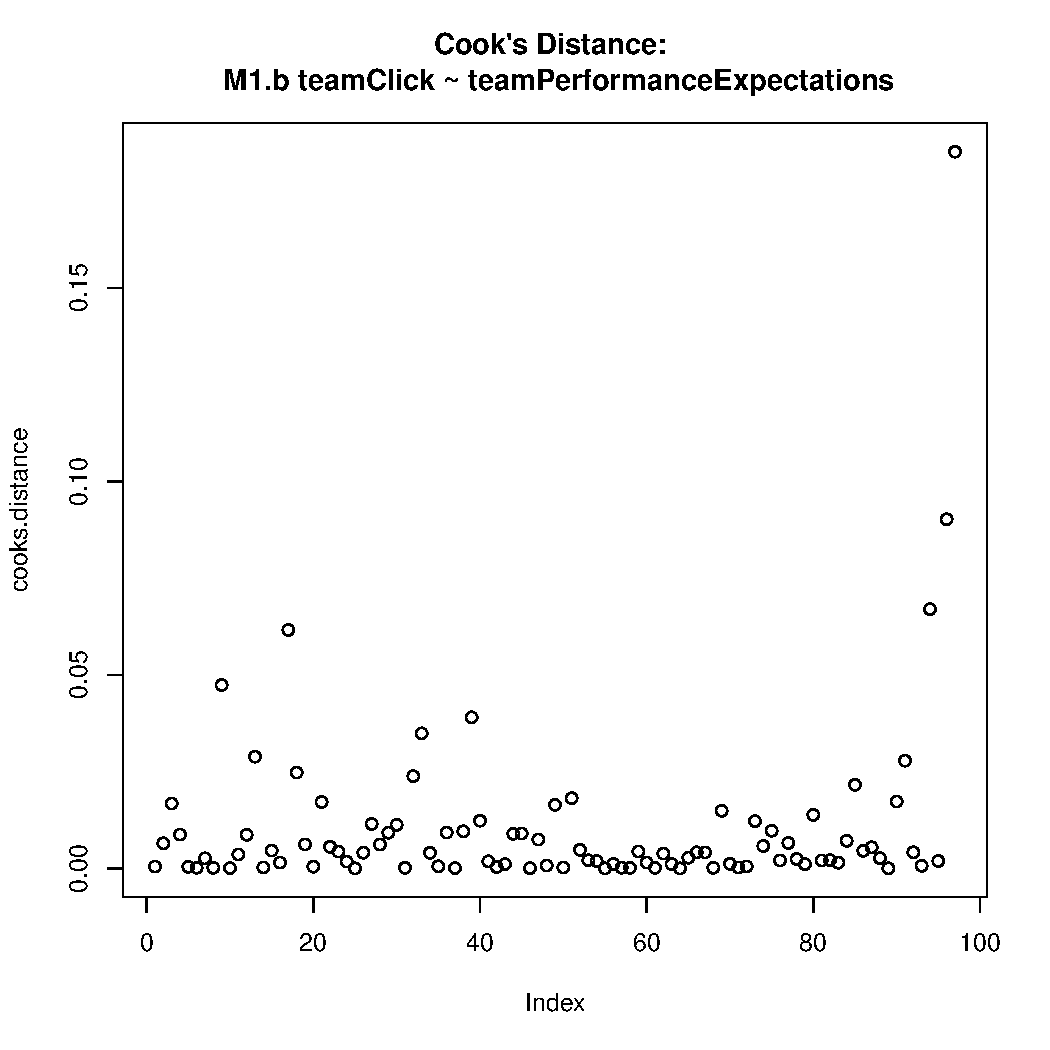
\includegraphics[scale =.4]{images/MLM1bCooksD.pdf}
         \caption{Model assumptions: Model 1.b Team Performance Expectations predict Team Click}
         \label{fig:MLM1bAssumptions}
       \end{figure}



       \subsubsection{Pre- to Post Tournament\label{app8:MLM21b}}

      % 
% Table created by stargazer v.5.2 by Marek Hlavac, Harvard University. E-mail: hlavac at fas.harvard.edu
% Date and time: Tue, Jun 27, 2017 - 09:21:13
\begin{table}[!htbp] \centering 
  \caption{M2.1b cTeamClick ~ cPerformanceExpectations} 
  \label{tab:MLM21bcTeamPerfExpcClick} 
\begin{tabular}{@{\extracolsep{5pt}}lccc} 
\\[-1.8ex]\hline 
\hline \\[-1.8ex] 
 & \multicolumn{3}{c}{\textit{Dependent variable:}} \\ 
\cline{2-4} 
\\[-1.8ex] & \multicolumn{3}{c}{cTeamClick} \\ 
\\[-1.8ex] & (1) & (2) & (3)\\ 
\hline \\[-1.8ex] 
 (constant) & 0.10 & $-$0.57 & $-$0.64 \\ 
  & (0.13) & (0.30) & (0.44) \\ 
  & & & \\ 
 cTeamPerformanceExpectations &  & 0.01$^{*}$ & 0.01$^{*}$ \\ 
  &  & (0.004) & (0.005) \\ 
  & & & \\ 
 cIndPerformanceExpectations &  &  & $-$0.003 \\ 
  &  &  & (0.004) \\ 
  & & & \\ 
 objectiveCompetence &  &  & $-$0.13 \\ 
  &  &  & (0.11) \\ 
  & & & \\ 
 subjectiveCompetence &  &  & $-$0.16 \\ 
  &  &  & (0.09) \\ 
  & & & \\ 
 finalRank &  &  & 0.02 \\ 
  &  &  & (0.06) \\ 
  & & & \\ 
 minutesTotal &  &  & 0.003 \\ 
  &  &  & (0.005) \\ 
  & & & \\ 
 pointsTotal &  &  & 0.003 \\ 
  &  &  & (0.01) \\ 
  & & & \\ 
\hline \\[-1.8ex] 
Marginal R-squared &  &  & .40 \\ 
Conditional R-squared &  &  & .47 \\ 
Observations & 99 & 99 & 97 \\ 
Log Likelihood & $-$130.59 & $-$127.00 & $-$123.15 \\ 
Akaike Inf. Crit. & 267.19 & 266.01 & 270.30 \\ 
Bayesian Inf. Crit. & 274.97 & 281.58 & 301.20 \\ 
\hline 
\hline \\[-1.8ex] 
\textit{Note:}  & \multicolumn{3}{r}{$^{*}$p$<$0.05; $^{**}$p$<$0.01; $^{***}$p$<$0.001} \\ 
\end{tabular} 
\end{table} 

       
\begin{table}
\begin{center}
\begin{tabular}{l c c c }
\toprule
 & Controls & Log-adjusted & Outliers removed \\
\midrule
(constant)                                 & $0.33$               & $\mathbf{1.27}^{***}$ & $0.40$                \\
                                           & $(0.51)$             & $(0.16)$              & $(0.39)$              \\
Team Performance Vs Expectations           & $\mathbf{0.30}^{**}$ & $\mathbf{0.09}^{*}$   & $\mathbf{0.32}^{***}$ \\
                                           & $(0.11)$             & $(0.04)$              & $(0.08)$              \\
Ind Performance Vs Expectations            & $-0.10$              & $-0.03$               & $\mathbf{-0.22}^{**}$ \\
                                           & $(0.10)$             & $(0.03)$              & $(0.08)$              \\
Objective Competence                       & $-0.15$              & $-0.05$               & $0.03$                \\
                                           & $(0.12)$             & $(0.04)$              & $(0.10)$              \\
Subjective Competence                      & $-0.15$              & $-0.05$               & $-0.03$               \\
                                           & $(0.09)$             & $(0.03)$              & $(0.08)$              \\
Final Rank                                 & $-0.01$              & $-0.00$               & $-0.08$               \\
                                           & $(0.06)$             & $(0.02)$              & $(0.04)$              \\
Minutes Total                              & $0.00$               & $0.00$                & $-0.00$               \\
                                           & $(0.01)$             & $(0.00)$              & $(0.00)$              \\
Points Total                               & $0.00$               & $0.00$                & $0.01$                \\
                                           & $(0.01)$             & $(0.00)$              & $(0.01)$              \\
Fatigue                                    & $-0.08$              & $-0.00$               & $-0.07$               \\
                                           & $(0.11)$             & $(0.04)$              & $(0.09)$              \\
Extraverted                                & $-0.06$              & $-0.02$               & $0.01$                \\
                                           & $(0.07)$             & $(0.02)$              & $(0.05)$              \\
\midrule
AIC                                        & 253.92               & 50.47                 & 200.30                \\
BIC                                        & 288.92               & 85.47                 & 234.66                \\
Log Likelihood                             & -112.96              & -11.23                & -86.15                \\
Num. obs.                                  & 90                   & 90                    & 86                    \\
Num. groups: team                          & 13                   & 13                    & 13                    \\

\bottomrule
\multicolumn{4}{l}{\scriptsize{Coefficients with $p < 0.05$ in \textbf{bold}. Effect size of model excluding outliers: Marginal $R^2 = .17$, Conditional $R^2 = .20$}}
\end{tabular}
\caption{Prediction 2: Team Click Change predicts Social Bonding Change in the Post-Tournament survey data (n = 90).}
\label{tab:MLM21bOutLogComparison}
\end{center}
\end{table}



       %\begin{figure}[htbp]

        %\end{figure} 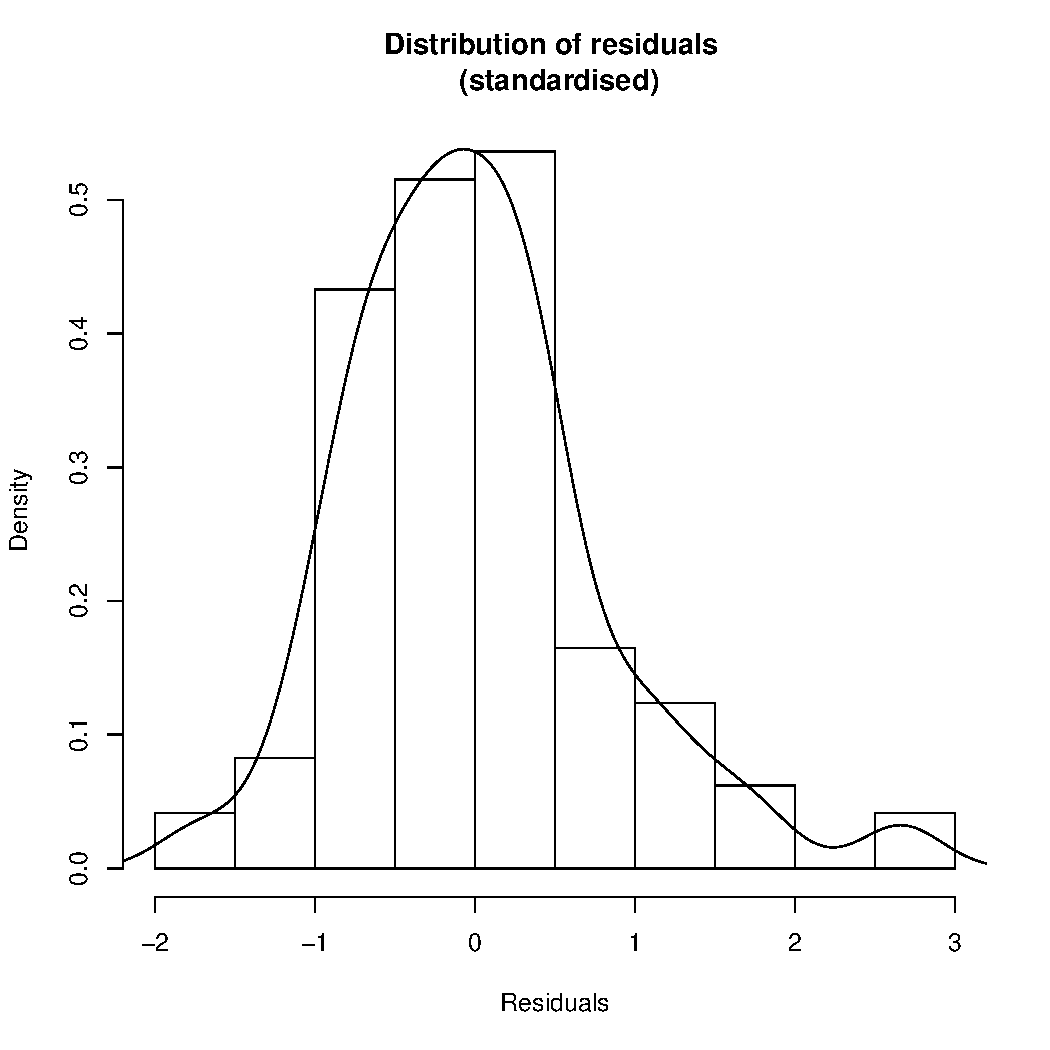
\includegraphics[scale =.4]{images/MLM21bHist.pdf}
        % 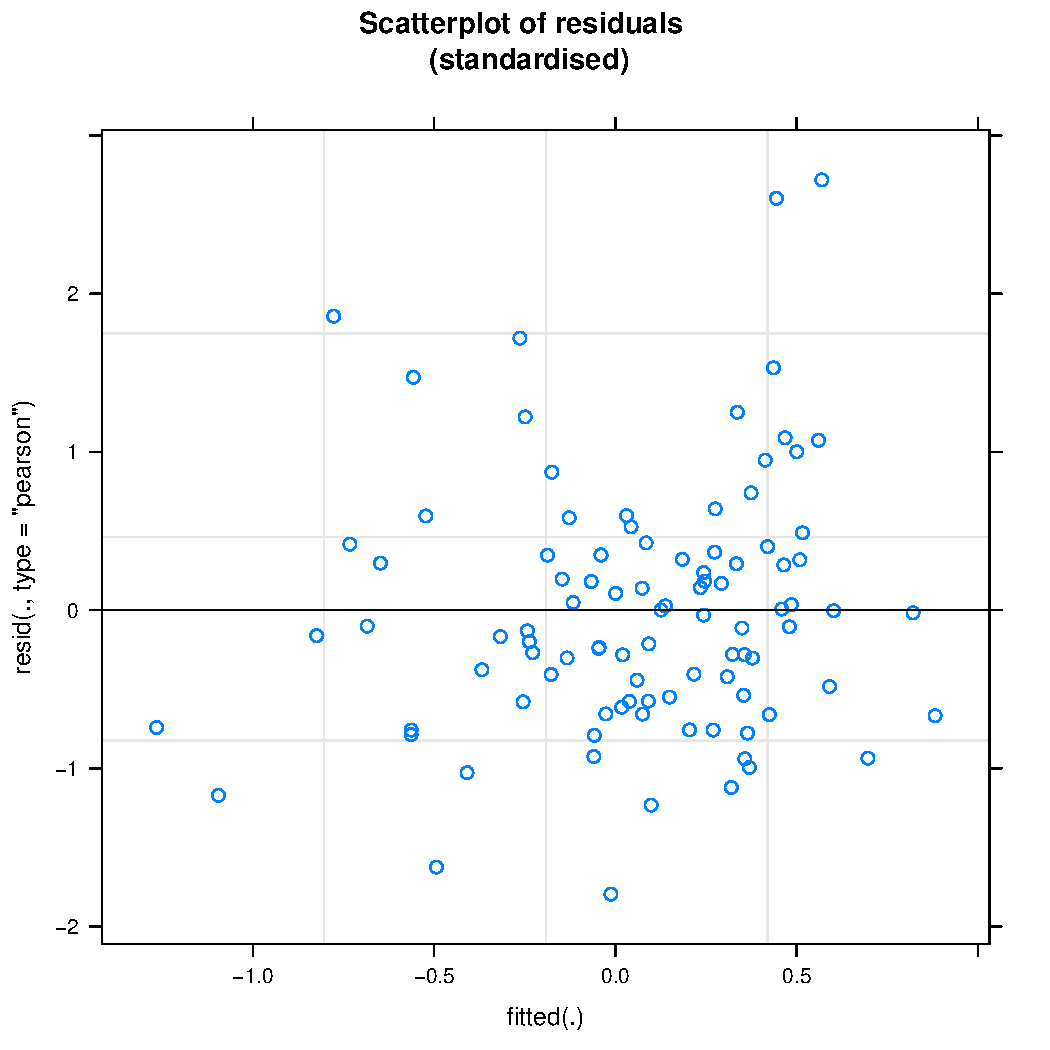
\includegraphics[scale =.4]{images/MLM21bScatter.pdf}
        % 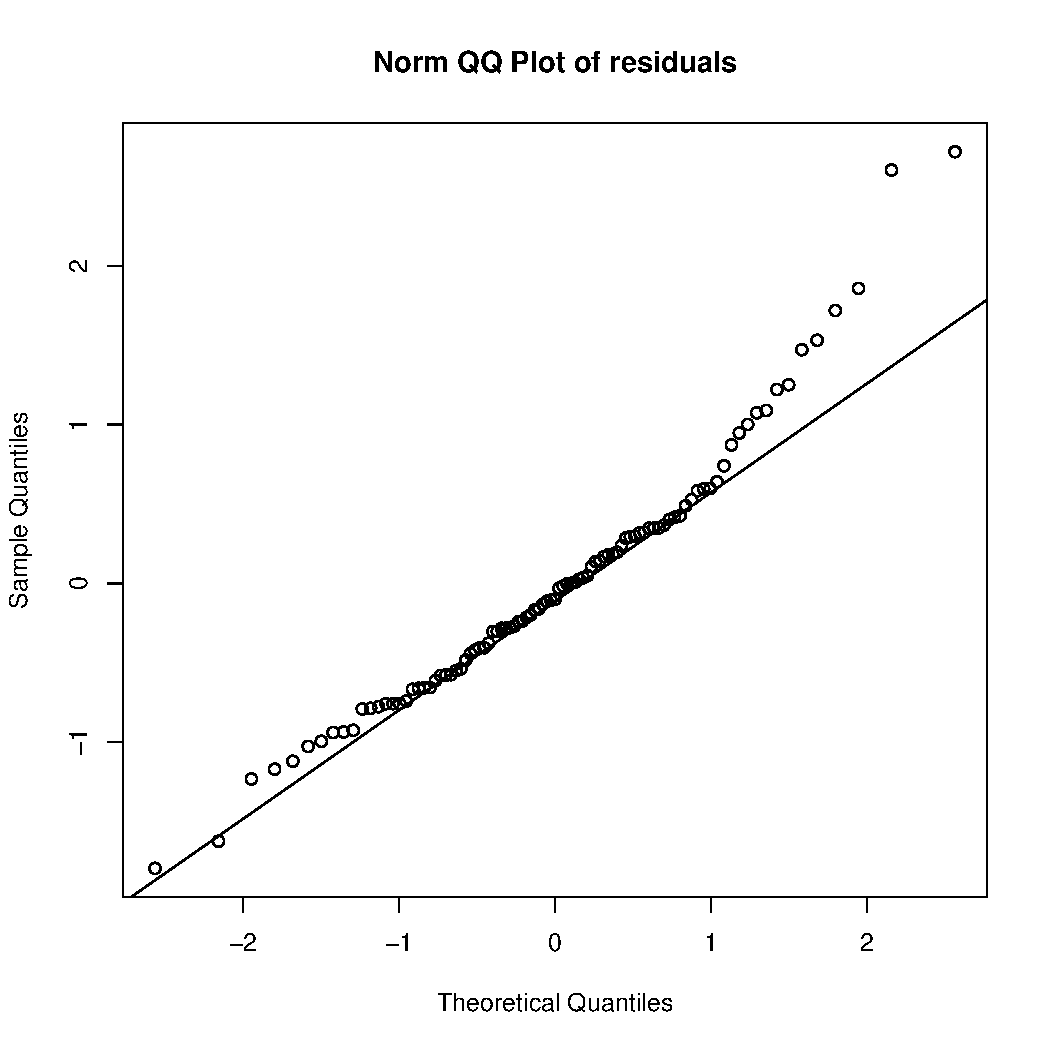
\includegraphics[scale =.4]{images/MLM21bQQNorm.pdf}
        % 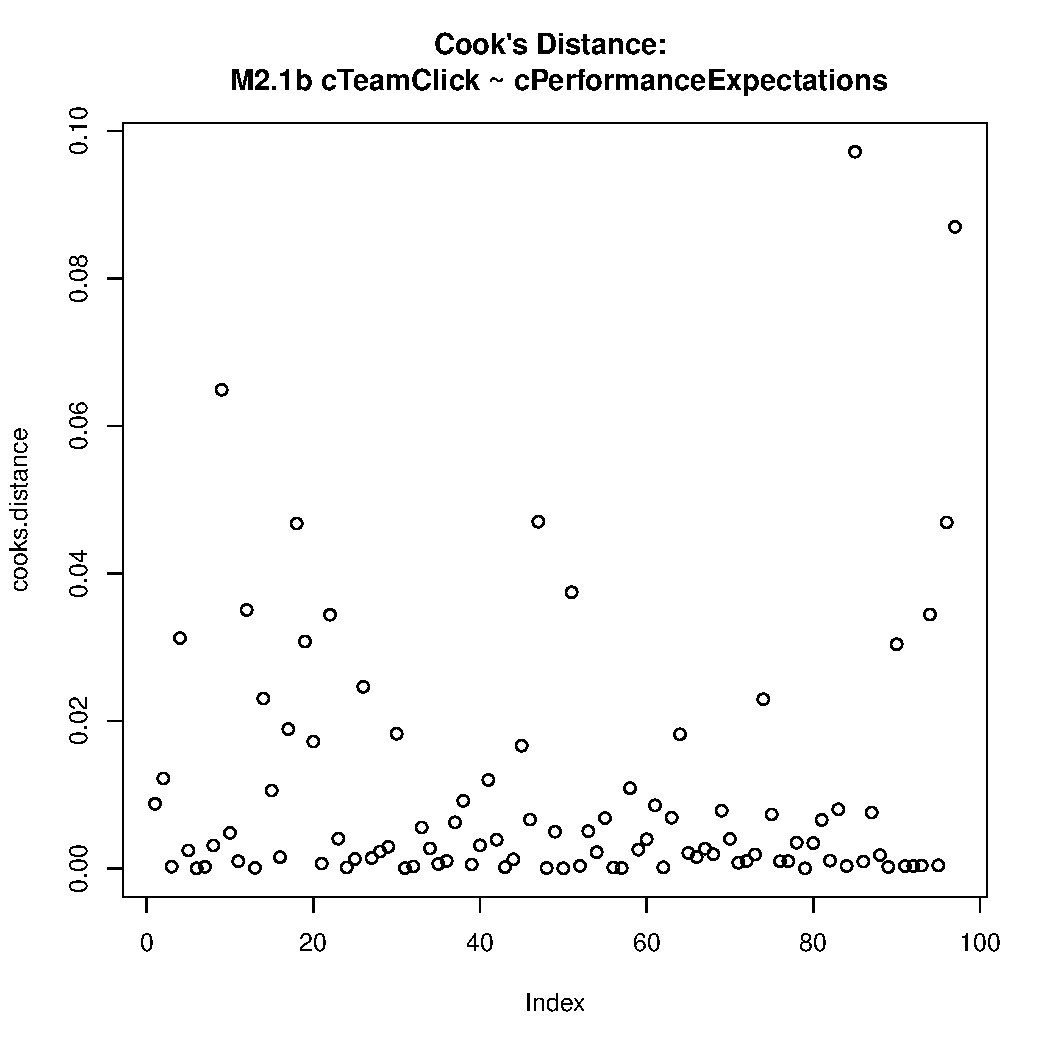
\includegraphics[scale =.4]{images/MLM21bCooksD.pdf}
        % \caption{Model assumptions: M2.1b Team Performance %Expectations Post-Tournament predicts change in Team Click}
      %   \label{fig:MLM21bAssumptions}
       %\end{figure}


       \begin{figure}[htbp]
         \includegraphics[scale =.4]{images/MLM21bOutHist.pdf}
         \includegraphics[scale =.4]{images/MLM21bOutScatter.pdf}
         \includegraphics[scale =.4]{images/MLM21bOutQQNorm.pdf}
         \includegraphics[scale =.4]{images/MLM21bOutCooksD.pdf}
         \caption{Model assumptions: M2.1b Team Performance Expectations Post-Tournament predicts change in Team Click (outliers removed)}
         \label{fig:MLM21bOutAssumptions}
       \end{figure}





       \subsubsection{Overall Tournament}


      %     \begin{align*}
      %       Team Click =  Team Performance Expectations  \\
      %                 + Individual Performance Expectations   \\
      %                 + Objective Competence + Subjective Competence \\
      %                 + TournamentPerformanceMeasures  \\
      %     \end{align*}


         
\begin{table}
\begin{center}
\begin{tabular}{l c c c }
\toprule
 & Intercept & Main effect & Controls \\
\midrule
(constant)                                                        & $-0.00$  & $-0.06$               & $-0.12$               \\
                                                                  & $(0.04)$ & $(0.03)$              & $(0.21)$              \\
Team Performance Vs Expectations                                  &          & $\mathbf{0.74}^{***}$ & $\mathbf{0.72}^{***}$ \\
                                                                  &          & $(0.03)$              & $(0.05)$              \\
Ind Performance Vs Expectations                                   &          &                       & $\mathbf{0.12}^{**}$  \\
                                                                  &          &                       & $(0.04)$              \\
Objective Competence                                              &          &                       & $0.04$                \\
                                                                  &          &                       & $(0.04)$              \\
Subjective Competence                                             &          &                       & $0.07$                \\
                                                                  &          &                       & $(0.04)$              \\
Final Rank                                                        &          &                       & $-0.00$               \\
                                                                  &          &                       & $(0.02)$              \\
Minutes Total                                                     &          &                       & $-0.00$               \\
                                                                  &          &                       & $(0.00)$              \\
Points Total                                                      &          &                       & $0.00$                \\
                                                                  &          &                       & $(0.00)$              \\
Fatigue                                                           &          &                       & $0.00$                \\
                                                                  &          &                       & $(0.00)$              \\
Extraverted                                                       &          &                       & $0.01$                \\
                                                                  &          &                       & $(0.03)$              \\
\midrule
AIC                                                               & 1552.70  & 842.67                & 602.59                \\
BIC                                                               & 1570.04  & 879.53                & 665.89                \\
Log Likelihood                                                    & -772.35  & -412.33               & -284.30               \\
Num. obs.                                                         & 564      & 444                   & 306                   \\
\bottomrule
\multicolumn{4}{l}{\scriptsize{Coefficients with $p < 0.05$ in \textbf{bold}. Marginal $R^2 = .63$, Conditional $R^2 = .69$}}
\end{tabular}
\caption{Prediction 1: Team Performance Vs Expectations predicts Team Click in the Overall Tournament survey data (n = 90).}
\label{tab:MLM31ateamPerfClickTournament}
\end{center}
\end{table}



       \begin{figure}[htbp]
         \includegraphics[scale =.4]{images/MLM31aHist.pdf}
         \includegraphics[scale =.4]{images/MLM31aScatter.pdf}
         \includegraphics[scale =.4]{images/MLM31aQQNorm.pdf}
         \includegraphics[scale =.4]{images/MLM31aCooksD.pdf}
         \caption{Model assumptions: Team Performance Vs Expectations predict Team Click}
         \label{fig:MLM31aAssumptions}
       \end{figure}








      \subsection{Prediction 5.2: More positive perceptions of Team Performance Components will predict higher levels of social bonding}



%\subsubsection{Post-Tournament}

    %  \myparagraph{LMER model}
    %      \myparagraph{Model comparisons}
    %      \newgeometry{margin=0.5cm}
    %      
% Table created by stargazer v.5.2 by Marek Hlavac, Harvard University. E-mail: hlavac at fas.harvard.edu
% Date and time: Tue, Jun 27, 2017 - 17:01:54
\begin{table}[!htbp] \centering 
  \caption{M3.b socialBonding = teamPerformanceExpectations} 
  \label{tab:MLM3bExpectationsBonding} 
\scriptsize 
\begin{tabular}{@{\extracolsep{5pt}}lccc} 
\\[-1.8ex]\hline 
\hline \\[-1.8ex] 
 & \multicolumn{3}{c}{\textit{Dependent variable:}} \\ 
\cline{2-4} 
\\[-1.8ex] & socialBonding & bondingPostFactorOut & bondingPostFactorLogReturned \\ 
 &  & outliers removed & log-transformed \\ 
\\[-1.8ex] & (1) & (2) & (3)\\ 
\hline \\[-1.8ex] 
 (constant) & $-$1.67$^{*}$ & $-$1.18$^{*}$ & 1.19$^{***}$ \\ 
  & (0.73) & (0.53) & (0.31) \\ 
  & & & \\ 
 teamPerformanceExpectations & 0.01$^{*}$ & 0.01$^{**}$ & 0.01$^{**}$ \\ 
  & (0.01) & (0.004) & (0.003) \\ 
  & & & \\ 
 individualPerformanceExpectations & 0.004 & 0.001 & 0.001 \\ 
  & (0.004) & (0.003) & (0.002) \\ 
  & & & \\ 
 objectiveCompetence & 0.03 & 0.02 & 0.02 \\ 
  & (0.10) & (0.07) & (0.04) \\ 
  & & & \\ 
 subjectiveCompetence & 0.19$^{*}$ & 0.12 & 0.08$^{*}$ \\ 
  & (0.09) & (0.06) & (0.04) \\ 
  & & & \\ 
 finalRank & 0.08 & 0.10 & 0.04 \\ 
  & (0.13) & (0.09) & (0.05) \\ 
  & & & \\ 
 minutesTotal & 0.0003 & 0.001 & 0.0001 \\ 
  & (0.004) & (0.003) & (0.002) \\ 
  & & & \\ 
 pointsTotal & $-$0.04 & $-$0.06 & $-$0.03 \\ 
  & (0.09) & (0.06) & (0.04) \\ 
  & & & \\ 
 pointsTotal & $-$0.001 & $-$0.004 & $-$0.002 \\ 
  & (0.01) & (0.005) & (0.003) \\ 
  & & & \\ 
\hline \\[-1.8ex] 
Marginal R-squared & .20 & .19 & .23 \\ 
Conditional R-squared & .40 & .40 & .44 \\ 
Observations & 97 & 91 & 97 \\ 
Log Likelihood & $-$117.26 & $-$77.84 & $-$32.42 \\ 
Akaike Inf. Crit. & 260.52 & 181.67 & 90.85 \\ 
Bayesian Inf. Crit. & 293.99 & 214.31 & 124.32 \\ 
\hline 
\hline \\[-1.8ex] 
\textit{Note:}  & \multicolumn{3}{r}{$^{*}$p$<$0.05; $^{**}$p$<$0.01; $^{***}$p$<$0.001} \\ 
\end{tabular} 
\end{table} 

    %      \restoregeometry

    %  \myparagraph{Model robustness checks}


    %  \begin{figure}[htbp]
    %    \includegraphics[scale =.4]{images/MLM3bHist.pdf}
    %    \includegraphics[scale =.4]{images/MLM3bScatter.pdf}
    %    \includegraphics[scale =.4]{images/MLM3bQQNorm.pdf}
    %    \includegraphics[scale =.4]{images/MLM3bCooksD.pdf}
    %    \caption{Model assumptions: Team Performance Components predicts Social Bonding }
    %    \label{fig:MLM3bAssumptions}
    %  \end{figure}

    %  \begin{figure}[htbp]
    %    \includegraphics[scale =.4]{images/MLM3bLogHist.pdf}
    %    \includegraphics[scale =.4]{images/MLM3bLogScatter.pdf}
    %    \includegraphics[scale =.4]{images/MLM3bLogQQNorm.pdf}
    %    \includegraphics[scale =.4]{images/MLM3bLogCooksD.pdf}
    %    \caption{Log-transformed model assumptions: Team Performance Components predicts Social Bonding}
    %    \label{fig:MLM3bLogAssumptions}
    %  \end{figure}




      \subsubsection{Pre- to Post Tournament\label{app8:MLM23b}}

          %\newgeometry{margin=0.5cm}
        %  
% Table created by stargazer v.5.2 by Marek Hlavac, Harvard University. E-mail: hlavac at fas.harvard.edu
% Date and time: Tue, Jun 27, 2017 - 17:15:15
\begin{table}[!htbp] \centering 
  \caption{cSocialBonding ~ teamPerformanceExpectations} 
  \label{tab:MLM23bcBondingteamPerfExp} 
\scriptsize 
\begin{tabular}{@{\extracolsep{5pt}}lccccc} 
\\[-1.8ex]\hline 
\hline \\[-1.8ex] 
 & \multicolumn{5}{c}{\textit{Dependent variable:}} \\ 
\cline{2-6} 
\\[-1.8ex] & \multicolumn{3}{c}{cSocialBonding} & bondingPostFactorLogReturned & bondingFactorChangePrePostOut \\ 
\\[-1.8ex] & (1) & (2) & (3) & (4) & (5)\\ 
\hline \\[-1.8ex] 
 (constant) & 0.34$^{***}$ & $-$0.07 & 0.01 & 1.34$^{***}$ & $-$0.01 \\ 
  & (0.09) & (0.25) & (0.39) & (0.22) & (0.33) \\ 
  & & & & & \\ 
 teamPerformanceExpectations &  & 0.01$^{*}$ & 0.01$^{*}$ & 0.01$^{***}$ & 0.005 \\ 
  &  & (0.004) & (0.004) & (0.003) & (0.004) \\ 
  & & & & & \\ 
 indPerformanceExpectations &  &  & $-$0.004 & 0.001 & $-$0.0000 \\ 
  &  &  & (0.004) & (0.002) & (0.003) \\ 
  & & & & & \\ 
 objectiveCompetence &  &  & 0.03 & 0.01 & 0.04 \\ 
  &  &  & (0.11) & (0.04) & (0.08) \\ 
  & & & & & \\ 
 subjectiveCompetence &  &  & $-$0.06 & 0.09$^{**}$ & $-$0.03 \\ 
  &  &  & (0.10) & (0.04) & (0.07) \\ 
  & & & & & \\ 
 finalRank &  &  & $-$0.03 & 0.01 & $-$0.03 \\ 
  &  &  & (0.05) & (0.02) & (0.04) \\ 
  & & & & & \\ 
 minutesTotal &  &  & 0.004 & 0.0003 & 0.001 \\ 
  &  &  & (0.005) & (0.002) & (0.003) \\ 
  & & & & & \\ 
 pointsTotal &  &  & 0.002 & $-$0.002 & $-$0.0003 \\ 
  &  &  & (0.01) & (0.003) & (0.01) \\ 
  & & & & & \\ 
\hline \\[-1.8ex] 
Marginal R-squared &  & .03 & .05 & .23 &  \\ 
Conditional R-squared &  & .03 & .05 & .46 &  \\ 
Observations & 99 & 99 & 97 & 97 & 86 \\ 
Log Likelihood & $-$129.78 & $-$128.30 & $-$125.20 & $-$32.67 & $-$75.13 \\ 
Akaike Inf. Crit. & 265.55 & 268.60 & 274.39 & 89.34 & 174.25 \\ 
Bayesian Inf. Crit. & 273.34 & 284.17 & 305.29 & 120.24 & 203.70 \\ 
\hline 
\hline \\[-1.8ex] 
\textit{Note:}  & \multicolumn{5}{r}{$^{*}$p$<$0.1; $^{**}$p$<$0.05; $^{***}$p$<$0.01} \\ 
\end{tabular} 
\end{table} 

% Table created by stargazer v.5.2 by Marek Hlavac, Harvard University. E-mail: hlavac at fas.harvard.edu
% Date and time: Tue, Jun 27, 2017 - 17:15:15
\begin{table}[!htbp] \centering 
  \caption{cSocialBonding ~ teamPerformanceExpectations} 
  \label{tab:MLM23bcBondingteamPerfExp} 
\scriptsize 
\begin{tabular}{@{\extracolsep{5pt}} ccc} 
\\[-1.8ex]\hline 
\hline \\[-1.8ex] 
$0.05$ & $0.01$ & $0.001$ \\ 
\hline \\[-1.8ex] 
\end{tabular} 
\end{table} 

        %  \restoregeometry


      \begin{figure}[htbp]
        \includegraphics[scale =.4]{images/MLM23bLogHist.pdf}
        \includegraphics[scale =.4]{images/MLM23bLogScatter.pdf}
        \includegraphics[scale =.4]{images/MLM23bLogQQNorm.pdf}
        \includegraphics[scale =.4]{images/MLM23bLogCooksD.pdf}
        \caption{Log-transformed model assumptions: Team Performance Vs Expectations predicts Social Bonding}
        \label{fig:MLM3bLogAssumptions}
      \end{figure}


      \subsubsection{Overall Tournament\label{app8:MLM32a}}


       
\begin{table}
\begin{center}
\begin{tabular}{l c c c c }
\toprule
 & Main effect & Controls & Log-transformed & Log and outliers \\
\midrule
(constant)                        & $-0.00$               & $\mathbf{0.51}^{*}$   & $\mathbf{1.71}^{***}$ & $\mathbf{1.64}^{***}$ \\
                                  & $(0.04)$              & $(0.26)$              & $(0.06)$              & $(0.08)$              \\
Team Performance Vs Expectations  & $\mathbf{0.59}^{***}$ & $\mathbf{0.47}^{***}$ & $\mathbf{0.11}^{***}$ & $\mathbf{0.07}^{***}$ \\
                                  & $(0.04)$              & $(0.06)$              & $(0.01)$              & $(0.02)$              \\
Ind Performance Vs Expectations   &                       & $\mathbf{0.25}^{***}$ & $\mathbf{0.05}^{***}$ & $0.01$                \\
                                  &                       & $(0.06)$              & $(0.01)$              & $(0.02)$              \\
Objective Competence              &                       & $0.07$                & $0.02$                & $0.01$                \\
                                  &                       & $(0.05)$              & $(0.01)$              & $(0.02)$              \\
Subjective Competence             &                       & $0.09$                & $\mathbf{0.02}^{*}$   & $\mathbf{0.03}^{*}$   \\
                                  &                       & $(0.05)$              & $(0.01)$              & $(0.01)$              \\
Final Rank                        &                       & $-0.03$               & $-0.01$               & $-0.01$               \\
                                  &                       & $(0.02)$              & $(0.01)$              & $(0.01)$              \\
Minutes Total                   &                       & $-0.01$  & $-0.00$  & $-0.00$               \\
                                  &                       & $(0.00)$              & $(0.00)$              & $(0.00)$              \\
Points Total                      &                       & $0.00$                & $0.00$                & $0.00$                \\
                                  &                       & $(0.00)$              & $(0.00)$              & $(0.00)$              \\
Fatigue                           &                       & $0.00$                & $0.00$                & $0.00$                \\
                                  &                       & $(0.00)$              & $(0.00)$              & $(0.00)$              \\
Extraverted                       &                       & $-0.04$               & $-0.01$               & $-0.02$               \\
                                  &                       & $(0.03)$              & $(0.01)$              & $(0.01)$              \\
\midrule
AIC                               & 1083.79               & 752.42                & -131.94               & -8.28                 \\
BIC                               & 1104.27               & 800.83                & -83.53                & 38.54                 \\
Log Likelihood                    & -536.89               & -363.21               & 78.97                 & 17.14                 \\
Num. obs.                         & 444                   & 306                   & 306                   & 271                   \\
\bottomrule
\multicolumn{5}{l}{\scriptsize{Coefficients with $p < 0.05$ in \textbf{bold}. Effect sizes of the Log and outlier model: Marginal $R^2 = .36$, Conditional $R^2 = .36$}}
\end{tabular}
\caption{Prediction 3: Team Performance Vs Expectations predicts Social Bonding in the Overall Tournament survey data (n = 90).}
\label{tab:MLM32ateamPerfBondingTournament}
\end{center}
\end{table}

       %
% Table created by stargazer v.5.2 by Marek Hlavac, Harvard University. E-mail: hlavac at fas.harvard.edu
% Date and time: Thu, Sep 14, 2017 - 09:42:11
\begin{table}[!htbp] \centering 
  \caption{Model Comparison: M3.2a socialBondingTournament ~ teamPerformanceExpectationsTournament} 
  \label{tab:MLM32ateamPerfBondingTournamentModelComparison} 
\scriptsize 
\begin{tabular}{@{\extracolsep{5pt}}lccc} 
\\[-1.8ex]\hline 
\hline \\[-1.8ex] 
 & \multicolumn{3}{c}{\textit{Dependent variable:}} \\ 
\cline{2-4} 
 & model & log-transformed & outliers+log-transformed \\ 
\\[-1.8ex] & (1) & (2) & (3)\\ 
\hline \\[-1.8ex] 
 (constant) & $-$0.70$^{***}$ & 1.42$^{***}$ & 1.42$^{***}$ \\ 
  & (0.18) & (0.04) & (0.06) \\ 
  & & & \\ 
 teamPerformanceExpectations & 0.01$^{***}$ & 0.003$^{***}$ & 0.003$^{***}$ \\ 
  & (0.002) & (0.0005) & (0.001) \\ 
  & & & \\ 
 indPerformanceExpectations & 0.01$^{**}$ & 0.001$^{**}$ & 0.0001 \\ 
  & (0.002) & (0.0004) & (0.001) \\ 
  & & & \\ 
 objectiveCompetence & 0.04 & 0.01 & 0.01 \\ 
  & (0.05) & (0.01) & (0.02) \\ 
  & & & \\ 
 subjectiveCompetence & 0.10$^{*}$ & 0.03$^{*}$ & 0.03$^{*}$ \\ 
  & (0.04) & (0.01) & (0.01) \\ 
  & & & \\ 
 finalRank & $-$0.04 & $-$0.01 & $-$0.01 \\ 
  & (0.02) & (0.005) & (0.01) \\ 
  & & & \\ 
 minutesTotal & $-$0.003 & $-$0.001 & $-$0.001 \\ 
  & (0.002) & (0.001) & (0.001) \\ 
  & & & \\ 
 pointsTotal & 0.001 & 0.0001 & 0.0000 \\ 
  & (0.004) & (0.001) & (0.001) \\ 
  & & & \\ 
\hline \\[-1.8ex] 
Marginal R-squared & .33 & .11 & .09 \\ 
Conditional R-squared & .53 & .23 & .17 \\ 
Shapiro-Wilk Test (p-value) & .97($<$.00001) & .96($<$.00001) & .97($<$.00001) \\ 
Observations & 331 & 331 & 294 \\ 
Log Likelihood & $-$373.85 & 96.45 & 21.56 \\ 
Akaike Inf. Crit. & 777.70 & $-$162.91 & $-$13.13 \\ 
Bayesian Inf. Crit. & 834.73 & $-$105.88 & 42.13 \\ 
\hline 
\hline \\[-1.8ex] 
\textit{Note:}  & \multicolumn{3}{r}{$^{*}$p$<$0.05; $^{**}$p$<$0.01; $^{***}$p$<$0.001} \\ 
\end{tabular} 
\end{table} 



    \begin{figure}[htbp]
   \includegraphics[scale =.4]{images/MLM32aHist.pdf}
        \includegraphics[scale =.4]{images/MLM32aScatter.pdf}
        \includegraphics[scale =.4]{images/MLM32aQQNorm.pdf}
        \includegraphics[scale =.4]{images/MLM32aCooksD.pdf}
        \caption{Model assumptions: Team Performance Vs Expectations predicts Social Bonding}
     \label{fig:MLM3bLogAssumptions}
    \end{figure}


      \end{CJK}
